%%%%%%%%%%%%%%%%%%%%%%%%%%%%%%%%%%%%%%%%%%%%%%%%%%%%%%%%%%%%%%%%%%%%%%%%
%%                                                                    %%
%% This is file `ucalgarythesis.tex'  -- a document template for      %%
%% graduate theses at the University of Calgary.                      %%
%%                                                                    %%
%% This template document is to be used in conjunction with the       %%
%% thesis class file `ucalgarythesis.cls'.                            %%
%%                                                                    %%
%% Created by M.W. Girard, last updated 10 April 2016.                %%
%%                                                                    %%
%% This template was created to be in compliance with the University  %%
%% of Calgary thesis guidelines (version 14 April 2014)               %%
%%       https://grad.ucalgary.ca/current/thesis/guidelines.          %%
%%                                                                    %%
%%%%%%%%%%%%%%%%%%%%%%%%%%%%%%%%%%%%%%%%%%%%%%%%%%%%%%%%%%%%%%%%%%%%%%%%
%%                                                                    %%
%% By default, the text of the thesis is doublespaced and should be   %%
%% printed single-sided. All margins must be exactly one inch on all  %%
%% sides, and should not be bound or have binding edges. This is      %%
%% required by the University of Calgary thesis guidelines.           %%
%% All theses are now required to be submitted electronically.        %%
%%                                                                    %%
%%%%%%%%%%%%%%%%%%%%%%%%%%%%%%%%%%%%%%%%%%%%%%%%%%%%%%%%%%%%%%%%%%%%%%%%


%%%%%%%%%%%%%%%%%%%%%%%%%%%%%%%%%%%%%%%%%%%%%%%%%%%%%%%%%%%%
%%
%% Load the `ucalgarythesis.cls' document class
%%%%%%%%%%%%%%%%%%%%%%%%%%%%%%%%%%%%%%%%%%%%%%%%%%%%%%%%%%%%

\documentclass{ucalgarythesis}

%%%%%%%%%%%%%%%%%%%%%%%%%%%%%%%%%%%%%%%%%%%%%%%%%%%%%%%%%%%%%%%%%%%%%%
%% If you would like to print a personal copy of your thesis for    %%
%% your own record, you may print it double-sided and with extra    %%
%% margins for binding. Use the following line instead of the above %%
%% \documentclass{ucalgarythesis} for compiling personal copies of  %%
%% the thesis to be printed double-sided and bound.                 %%
%%%%%%%%%%%%%%%%%%%%%%%%%%%%%%%%%%%%%%%%%%%%%%%%%%%%%%%%%%%%%%%%%%%%%%
%\documentclass[twoside,binding]{ucalgarythesis}

%%%%%%%%%%%%%%%%%%%%%%%%%%%%%%%%%%%%%%%%%%%%%%%%%%%%%%%%%%%%
%%
%% Imported packages & custom user commands
%%%%%%%%%%%%%%%%%%%%%%%%%%%%%%%%%%%%%%%%%%%%%%%%%%%%%%%%%%%%

%% Include extra packages here

\usepackage[utf8]{inputenc}
\usepackage{amssymb,amsthm,amsmath}
%\usepackage[hidelinks]{hyperref}
\usepackage{algorithm}
%\usepackage{algorithmic}
\usepackage{algpseudocode}
\usepackage{comment}
\usepackage{enumitem}
\usepackage{graphicx}
\usepackage{multirow}
\usepackage{pgfplots}
\usepackage{tikz-cd}

\usepackage[style=numeric, backend=biber]{biblatex}
\bibliography{biblio}
%\bibliographystyle{plain}

%\usepackage{biblatex}

%%  Include other user-defined commands here

\let\div\undefined
\renewcommand{\bar}{\overline}

\algnewcommand{\algorithmicgoto}{\textbf{go to}}
\algnewcommand{\GoTo}[1]{\algorithmicgoto~{#1}}

\DeclareMathOperator{\Char}{char}
\DeclareMathOperator{\Cl}{Cl}
\DeclareMathOperator{\coim}{coim}
\DeclareMathOperator{\coker}{coker}
\DeclareMathOperator{\Der}{Der}
\DeclareMathOperator{\Div}{Div}
\DeclareMathOperator{\div}{div}
\DeclareMathOperator{\Frac}{Frac}
\DeclareMathOperator{\Gal}{Gal}
\DeclareMathOperator{\Hom}{Hom}
\DeclareMathOperator{\Id}{Id}
\DeclareMathOperator{\im}{im}
\DeclareMathOperator{\lcm}{lcm}
\DeclareMathOperator{\Jac}{Jac}
\DeclareMathOperator{\LM}{LM}
\DeclareMathOperator{\LT}{LT}
\DeclareMathOperator{\Ker}{Ker}
\DeclareMathOperator{\nullity}{null}
\DeclareMathOperator{\Pic}{Pic}
\DeclareMathOperator{\Princ}{Princ}
\DeclareMathOperator{\orb}{orb}
\DeclareMathOperator{\ord}{ord}
\DeclareMathOperator{\rank}{rank}
\DeclareMathOperator{\supp}{supp}
\DeclareMathOperator{\Span}{Span}
\DeclareMathOperator{\type}{type}
%\DeclareMathOperator{\KVec}{K-Vec}

\newcommand{\inv}{^{-1}}
\newcommand{\pid}[1]{\left\langle #1 \right\rangle}

%\newcommand{\der}{\partial}
\newcommand{\defn}{\textbf}
\newcommand{\note}[1]{{\color{red}#1}}
\newcommand{\bb}[1]{\mathbb{#1}}
\newcommand{\tensor}[1]{\underset{#1}{\otimes}}
\renewcommand{\cal}[1]{\mathcal{#1}}

\theoremstyle{plain}
\newtheorem{theorem}{Theorem}[section]
\newtheorem{corollary}[theorem]{Corollary}
\newtheorem{conjecture}[theorem]{Conjecture}
\newtheorem{lemma}[theorem]{Lemma}
\newtheorem{proposition}[theorem]{Proposition}

\theoremstyle{definition}
\newtheorem{definition}[theorem]{Definition}
\newtheorem{example}[theorem]{Example}

\renewcommand*{\arraystretch}{0.8} % Adjust spacing between lines in matrices

\renewcommand\thesection{\arabic{section}} % Fix section/subsection numbering style
\renewcommand\thesubsection{\thesection.\arabic{subsection}}

%%%%%%%%%%%%%%%%%%%%%%%%%%%%%%%%%%%%%%%%%%%%%%%%%%%%%%%%%%%%%%%%%%%%%%%%
%%                                                                    %%
%% Begin document                                                     %%
%%                                                                    %%
%%%%%%%%%%%%%%%%%%%%%%%%%%%%%%%%%%%%%%%%%%%%%%%%%%%%%%%%%%%%%%%%%%%%%%%%
\begin{document}

%%%%%%%%%%%%%%%%%%%%%%%%%%%%%%%%%%%%%%%%%%%%%%%%%%%%%%%%%%%%%%%%%%%%%%%%
%%                                                                    %%
%% Title page                                                         %%
%%                                                                    %%
%%%%%%%%%%%%%%%%%%%%%%%%%%%%%%%%%%%%%%%%%%%%%%%%%%%%%%%%%%%%%%%%%%%%%%%%

%%%%%%%%%%%%%%%%%%%%%%%%%%%%%%%%%%%%%%%%%%%%%%%%%%%%%%%%%%%%%%%%%%%%%%%%
%% Instructions for title page information:                           %%
%%                                                                    %%
%%  Fill in the following fields with the required information:       %%
%%   - \title{...}        Title of the thesis                         %%
%%   - \author{...}       Your full name                              %%
%%   - \thesis{Thesis}    Type of document (may change to `Thesis' to %%
%%                           `Dissertation' depending on type of work)%%
%%   - \dept{...}         Full name of the graduate department or     %%
%%                           degree program                           %%
%%   - \degree{...}       Full name of the degree obtained            %%
%%                          (i.e. Doctor of Philosophy,               %%
%%                                 Master of Science, etc)            %%
%%   - \gradyear{...}     Year of submission                          %%
%%   - \monthname{...}    Month of submission                         %%
%%%%%%%%%%%%%%%%%%%%%%%%%%%%%%%%%%%%%%%%%%%%%%%%%%%%%%%%%%%%%%%%%%%%%%%%

\title{Divisor Class Group Arithmetic on $C_{3,4}$ Curves}
 
\author{Evan MacNeil}
\thesis{Thesis}
\dept{Graduate Program in Mathematics and Statistics}
\degree{Master of Science}
\gradyear{2019}
\monthname{August}


%%%%%%%%%%%%%%%%%%%%%%%%%%%%%%%%%%%%%%%%%%%%%%%%%%%  
%% Make the thesis title page.
%%%%%%%%%%%%%%%%%%%%%%%%%%%%%%%%%%%%%%%%%%%%%%%%%%%
\frontmatter           %% Don't remove this line.
\makethesistitle       %% Don't remove this line.


%%%%%%%%%%%%%%%%%%%%%%%%%%%%%%%%%%%%%%%%%%%%%%%%%%%%%%%%%%%%%%%%%%%%%%%%
%%                                                                    %%
%% Prefatory pages                                                    %%
%%                                                                    %%
%%%%%%%%%%%%%%%%%%%%%%%%%%%%%%%%%%%%%%%%%%%%%%%%%%%%%%%%%%%%%%%%%%%%%%%%
%% The following sections are in the correct order as specified by    %%
%% the April 2014 thesis guidelines set by the University of Calgary. %%
%%                                                                    %%
%% You may remove optional sections, but do not change the order.     %%
%%%%%%%%%%%%%%%%%%%%%%%%%%%%%%%%%%%%%%%%%%%%%%%%%%%%%%%%%%%%%%%%%%%%%%%%

%%%%%%%%%%%%%%%%%%%%%%%%%%%%%%%%%%%%%%%%%%%%%%%%%%%
%%
%% Abstract page (REQUIRED)
%%%%%%%%%%%%%%%%%%%%%%%%%%%%%%%%%%%%%%%%%%%%%%%%%%%

\begin{thesisabstract}  

Computing in the divisor class group of an algebraic curve is a non-trivial component in computing $L$-series.
$L$-series in turn are at the heart of the Sato-Tate conjecture and related conjectures.
The Sato-Tate conjecture has been proven for elliptic curves with complex multiplication,
but remains open for other families of algebraic curves.
In order to test these conjectures against other curve families, it is desirable to have efficient algorithms to perform divisor class group arithmetic.

Fast explicit formulas exist to perform divisor class group arithmetic for genus 1 and genus 2 curves.
However, the picture for genus 3 curves is incomplete.
Existing explicit formulas for arithmetic on non-hyperelliptic genus 3 curves ($C_{3,4}$ curves) have been developed with cryptographic applications in mind.
They make certain generacity assumptions on their inputs that hold with high probability in cryptographic settings,
but are unsuited for number theoretic use cases.
More general algorithms exist that can perform divisor class arithmetic over any curve, but they are slow.
The goal of this project is to bridge the gap --
to find fast explicit formulas describing $C_{3,4}$ curve arithmetic that are correct for all inputs.

\end{thesisabstract}


%%%%%%%%%%%%%%%%%%%%%%%%%%%%%%%%%%%%%%%%%%%%%%%%%%%
%%
%% Preface page (OPTIONAL)
%%%%%%%%%%%%%%%%%%%%%%%%%%%%%%%%%%%%%%%%%%%%%%%%%%%

%% This section is required if the work presented in the thesis is 
%% done as part of a collaboration. In this case, the preface must 
%% state which part of the thesis are the author's original work.
%% Otherwise this section is optional.

  \chapter{Preface}
 
  This thesis is an original work by the author. No part of this thesis has been previously published.
 
  % Some of the research conducted for this thesis forms part of an international research collaboration, led by Professor R.C. Smith at the University of Hogwarts
   
 
%%%%%%%%%%%%%%%%%%%%%%%%%%%%%%%%%%%%%%%%%%%%%%%%%%%
%%
%% Acknowledgements page (REQUIRED)
%%%%%%%%%%%%%%%%%%%%%%%%%%%%%%%%%%%%%%%%%%%%%%%%%%%

  \chapter{Acknowledgements}  
  
    [Don't forget to thank someone.]
    
%%%%%%%%%%%%%%%%%%%%%%%%%%%%%%%%%%%%%%%%%%%%%%%%%%
%%
%% Dedication page (this section is OPTIONAL)
%%%%%%%%%%%%%%%%%%%%%%%%%%%%%%%%%%%%%%%%%%%%%%%%%%

  \chapter[Dedication]{}
  
  \begin{dedication}
     \emph{To all the time I've wasted...}
  \end{dedication}

%%%%%%%%%%%%%%%%%%%%%%%%%%%%%%%%%%%%%%%%%%%%%%%%%%
%%
%% Various lists
%%%%%%%%%%%%%%%%%%%%%%%%%%%%%%%%%%%%%%%%%%%%%%%%%%
%% The Table of Contents and all Lists should be single spaced.

  \begin{singlespace}   %% Do not remove this line

%%%%%%%%%%%%%%%%%%%%%%%%%%%%%%%%%%%%%%%%%%%%%%%%%%
%%
%% Table of Contents (REQUIRED)
%%%%%%%%%%%%%%%%%%%%%%%%%%%%%%%%%%%%%%%%%%%%%%%%%%
  \renewcommand\contentsname{Table of Contents}
  \cleardoublepage\phantomsection
  \addcontentsline{toc}{chapter}{\contentsname}
  \tableofcontents

%%%%%%%%%%%%%%%%%%%%%%%%%%%%%%%%%%%%%%%%%%%%%%%%%%
%% List of figures (required, if any)
  \renewcommand{\listfigurename}{List of Figures and Illustrations}
  \cleardoublepage\phantomsection
  \addcontentsline{toc}{chapter}{\listfigurename}
  \listoffigures

%%%%%%%%%%%%%%%%%%%%%%%%%%%%%%%%%%%%%%%%%%%%%%%%%%
%% List of tables (required, if any)
  \renewcommand{\listtablename}{List of Tables}
  \cleardoublepage\phantomsection
  \addcontentsline{toc}{chapter}{\listtablename}
  \listoftables
  
%%%%%%%%%%%%%%%%%%%%%%%%%%%%%%%%%%%%%%%%%%%%%%%%%%
%% List of Symbols, abbreviations, and nomenclature (required, if any)   
%%
%% (Note: You may use your own format for your list of symbols, 
%%  abbreviations, etc. This format is just a guideline.)
%%
  \chapter{List of Symbols, Abbreviations and Nomenclature}      
  \begin{tabbing}
    Symbol or abbreviation~~~~~\= \ \ \ \ \ \ \ \ \ \ \ \ \ \ \ \ \ \ \ \ \ \ \ \ \ \ \ \ \ \ \ \ \ \ \ \  \parbox{5in}{Definition}\\

    \addsymbol \mbox{$\alpha$}: {The first letter of the Greek alphabet}
    \addsymbol \mbox{$\beta$}: {The second letter of the Greek alphabet}
    %
    % Add more symbols here...
    % . 
    % .
    % .
    %
    
    % Always keep the following line if you are using a list of symbols:
  \end{tabbing}
  
%%%%%%%%%%%%%%%%%%%%%%%%%%%%%%%%%%%%%%%%%%%%%%%%%%
%% End single spacing after last list
  \end{singlespace}     %% Do not remove this line
  
%%%%%%%%%%%%%%%%%%%%%%%%%%%%%%%%%%%%%%%%%%%%%%%%%%
%
% Epigraph (this section is OPTIONAL)
%%%%%%%%%%%%%%%%%%%%%%%%%%%%%%%%%%%%%%%%%%%%%%%%%%

  \chapter{Epigraph}

  \begin{epiquote} 
   \textit{A quotation is a handy thing to have about, saving one the trouble of thinking for oneself, always a laborious business.} 
  \end{epiquote}    
  \begin{flushright} - A.A. Milne, \textit{If I May}\end{flushright}\bigskip
   

%%%%%%%%%%%%%%%%%%%%%%%%%%%%%%%%%%%%%%%%%%%%%%%%%%%%%%%%%%%%%%%%%%%%%%%%
%%                                                                    %%
%% Main matter                                                        %%
%%                                                                    %%
%%%%%%%%%%%%%%%%%%%%%%%%%%%%%%%%%%%%%%%%%%%%%%%%%%%%%%%%%%%%%%%%%%%%%%%%

  \mainmatter           %% Do not remove this line
    
%%%%%%%%%%%%%%%%%%%%%%%%%%%%%%%%%%%%%%%%%%%%%%%%%%
%%
%% Chapters
%%%%%%%%%%%%%%%%%%%%%%%%%%%%%%%%%%%%%%%%%%%%%%%%%%

\setcounter{page}{12}

%%%%%%%%%%%%%%%%%%%%%%%%%%
%%%%%                %%%%%
%%%%%   Background   %%%%%
%%%%%                %%%%%
%%%%%%%%%%%%%%%%%%%%%%%%%%

\section{Background and Motivation}

\note{Generalizing Sato-Tate to higher genus curves requires Sato-Tate groups.
The theory is outside the scope of this thesis.}

A projective line over $\bb F_q$ has $q + 1$ rational points.
An elliptic curve over $\bb F_q$ has approximately as many rational points as does a line.
The actual number of rational points on an elliptic curve differs from that of the line by an error term
that is small compared to the size of the field $\bb F_q$.
The following theorem due to Hasse places bounds on this error term.
\begin{theorem}[Hasse's Theorem]
  Let $E$ be an elliptic curve over a finite field $\bb F_q$.
  The number of points on $E$ differs from $q + 1$ by at most $2 \sqrt q$.
  \[ | \#E(\bb F_q) - (q + 1) | \leq 2 \sqrt q \]
\end{theorem}

This theorem generalizes in the following way.
\begin{theorem}[Hasse-Weil Bound]
  Let $C$ be a curve of genus $g$ over a finite field $\bb F_q$.
  The number of points on $C$ differs from $q + 1$ by at most $2 g \sqrt q$.
  \[ | \#C(\bb F_q) - (q + 1) | \leq 2 g \sqrt q \]
\end{theorem}

Expressed differently, the Hasse-Weil Bound says that the quantity
\begin{equation}
  \frac {\#C(\bb F_q) - (q + 1)}{2 g \sqrt q}
\end{equation}
is between -1 and 1, so that for some angle $\theta_p$,
\begin{equation}
  \label{eq_sato_tate_ratio}
 \cos \theta_p = \frac {\#C(\bb F_q) - (q + 1)}{2 g \sqrt q}.
\end{equation}

Now given a fixed curve $C$, one can ask, what the probability is as $p$ varies that the error term should lie in some interval.
Given real numbers $-1 \leq a < b \leq 1$ (or angles $0 \leq \alpha < \beta \leq \pi$),
what is the probability that the ratio $\cos \theta_p \in [a, b]$ (or $\theta_p \in [\alpha, \beta]$)?
The Sato-Tate Conjecture (proven for genus 1), says that this probability follows a $\sin^2$ distribution.

\begin{conjecture}[Sato-Tate]
  Let $E$ be an elliptic curve without complex multiplication.
  \note{Complete this thought...}
  \[ \lim_{N \to \infty} \frac {\#\{ p \leq N : \alpha \leq \theta_p \leq \beta \}} {\pi(N)} = \frac 2 \pi \int_{\alpha}^{\beta} \sin^2 \theta\,d\theta. \]
\end{conjecture}

Divisor class group computations are used to compute the L-series of a genus 3 curve.
L-series is raised in
  * Birch and Swinnerton-Dyer conjecture
  * Koblitz-Zywina conjecture
  * Lang-Trotter conjecture
  * Sato-Tate conjecture
  

%%%%%%%%%%%%%%%%%%%%%%%%%%%%%%
%%%%%                    %%%%%
%%%%%   Groebner Bases   %%%%%
%%%%%                    %%%%%
%%%%%%%%%%%%%%%%%%%%%%%%%%%%%%

\section{Gr\"obner Bases}
\label{chap_groebner}

Divisors of $C_{3,4}$ curves will be represented by polynomial ideals.
Specifically, a divisor
\[ D = \sum n_iP_i - \left( \sum n_i \right) P^\infty \]
will be represented by the ideal of polynomials passing through each $P_i$ with multiplicity $n_i$.
We would like this representation to be unique.
Gr\"obner bases give such a representation.

A Gr\"obner basis for an ideal of polynomials $I$ is a generating set for $I$
satisfying some other properties described in Section \ref{sec:groebner_bases}.
Strictly speaking, a Gr\"obner basis is not a basis for $I$ (linear independence is not required),
though it does induce a basis for $R/I$.
An ideal has at least one Gr\"obner basis and possibly many, but it has a unique \emph{reduced} Gr\"obner basis.
Two ideals are equal if and only if they have the same reduced Gr\"obner basis.
Thus we will represent a divisor by a reduced Gr\"obner basis.

Gr\"obner bases are best understood in the context of another problem that they solve, the \defn{membership problem}.
Let $R$ be a multivariate polynomial ring over a field $K$,
  \[ R = K[x_1, \ldots, x_n], \]
and let $I$ be an ideal of $R$.
Given a polynomial $f \in R$, we wish to determine whether $f$ is a member of $I$.
We can examine the quotient ring $R/I$ and the image $\bar f$ of $f$ under the quotient map.
Certainly $f \in I$ if and only if, in the quotient ring, $\bar f \equiv 0$.

In the case of $R = \bb Z$ and $I = \pid m$, the image of an integer $n$ modulo $\pid m$ is the remainder of $n$ after long division by $m$.
We may conclude that $n \in \pid m$ if this remainder is 0.
In the case of $R = \bb C[x]$ and $I = \pid{g(x)}$, the image of a polynomial $f(x)$ moduloe $\pid{g(x)}$
is the remainder after polynomial long division by $g(x)$.
We may conclude that $f(x) \in \pid{g(x)}$ if this remainder is 0.
Essentially, the membership problem in these settings is solved by long division.
We would like to solve the membership problem for ideals of multivariate polynomial rings by a similar method.
In other words, we would like to generalize polynomial long division to a setting with multivariate polynomials.
This requires more than just considering dividing by a multivariate polynomial.
In the examples above, $\bb Z$ and $\bb C[x]$ are PIDs.
However, $\bb C[x,y]$ is not.
An ideal $I \subseteq \bb C[x,y]$ may have more than one generator, e.g. $I = \pid{x,y}$.
We must now also consider ''dividing'' by multiple polynomials.

We first make an observation regarding the Euclidean Algorithm in $K[x]$, for some field $K$.
The Euclidean Algorithm says that, given polynomials $f$ and $g$ in $K[x]$ ($g \neq 0$),
there exist unique polynomials $q$ and $r$ such that
  \[ f = qg + r \]
and such that either $r = 0$ or $\deg r < \deg g$.
This condition on $r$ can be equivalently (and more verbosely) expressed as
$r = 0$ or the largest monomial of $r$ does not divide the largest monomial of $g$.
This will be the basis of our generalization of polynomial long division,
but this requires making precise what we mean by ``largest monomial'' in a multivariate polynomial.

In the following subsections, we will discuss monomial orders and ideals of leading terms.
We will use this to describe a generalization of polynomial long division to multivariate polynomials.
We will immediately see that this generalization will not actually solve the membership problem, but it can be salvaged!
We will introduce Gr\"obner bases.
Then we will see how generalized polynomial long division solves our problem when the polynomials by which we are dividing form a Gr\"obner basis.



%%%%%%%%%%%%%%%%%%%%%%%%%%%%%%%%%%
%%%%%                        %%%%%
%%%%%   Monomial Orderings   %%%%%
%%%%%                        %%%%%
%%%%%%%%%%%%%%%%%%%%%%%%%%%%%%%%%%

\subsection{Monomial Orderings}

% References : Eisenbud \cite{eisenbud95} and Cox \cite{cox07}

When we write down a polynomial in one variable, we typically write the terms in increasing or decreasing order according to the terms' degrees.
One might write $3x^2 + x + 2$ or $2 + x + 3x^2$, for example, but typically not $x + 3x^2 + 3$.
It is natural to order terms according to their powers.

In a multivariate polynomial ring, there is no one ``natural'' way to order terms.
One could write an arbitrary bivariate quadratic in the order
  \[ ax^2 + bxy + cy^2 + dx + ey + f. \]
Here, terms are ordered according to their total degree.
Monomials of degree 2 come before those of degree 1, which in turn come before those of degree 0.
Within terms of the same degree, we write first the ones with the highest degree in $x$.
This is called a \defn{graded lexicographic order}.
We could get a different graded lexicographic order by prioritizing $y$ over $x$ among terms having the same degree, e.g.
  \[ cy^2 + bxy + ax^2 + ey + dx + f. \]

In some contexts, it makes sense to collect powers of $y$ and write instead
  \[ cy^2 + bxy + ey + ax^2 + dx + f. \]
This occurs in the context of, say, hyperelliptic curves, which are typically written in the form
  \[ y^2 + h(x)y = f(x). \]
Here, we first write the terms with the highest degree in $y$.
Within the terms having the same degree in $y$, we write first the terms having the highest degree in $x$.
This is a \defn{lexicographical order}.
Prioritizing $x$ over $y$ would yield a different lexicographical order,
  \[ ax^2 + bxy + dx + cy^2 + ey + f. \]

The two orders describe above are examples of monomial orders.
\begin{definition}
  Let $R = K[x_1, \ldots, x_n]$ be a polynomial ring.
  The \defn{set of (monic) monomials} of $R$ is the set
  \begin{equation*}
    \cal M_R := \left\{ \prod_{i=1}^n x_i^{k_i} ~|~ k_i \in \bb N \right\}.
  \end{equation*}
  
  A \defn{monomial order} is a total order $\leq$ on $\cal M_R$ such that for all monomials $a, b, c \in \cal M_R$:
  \begin{enumerate}[label=(\roman*)]
    \item $1 \leq a$, and
    \item $a \leq b \implies ac \leq bc$.
  \end{enumerate}
\end{definition}
Property (i) says that the order has a least element, specifically 1, and property (ii) asserts compatibility with multiplication.
\note{Eisenbud p.327 gives some motivation for this definition.}
Some authors define a monomial order to be a well-order,
but well-orderedness is a consequence of properties (i) and (ii).
\begin{proposition}
  Let $\leq$ be a monomial order. Then
  \label{prop_monomial_order}
  \begin{enumerate}[label=(\roman*)]
    \item
      if $a \leq b$ and $x \leq y$, then $ax \leq by$;
    \item
      $\leq$ is a well-order; and
    \item
      every strictly decreasing sequence of monomials
      \[ m_1 > m_2 > \dots \]
      eventually terminates.
  \end{enumerate}
\end{proposition}
\begin{proof}
  \begin{enumerate}[label=(\roman*)]
    \item
      Suppose $a \leq b$ and $x \leq y$.
      By property (ii), we have $ax \leq bx$ and $bx \leq by$.
      Total orders are transitive, so $ax \leq by$.
    
    \item
      (See \cite{eisenbud95} Lemma 15.2.)
      Let $M \subseteq \cal M$ be any subset of $R$'s monomials.
      
      Consider the $R$-ideal generated by $M$, $I = \pid M$.
      Since $R$ is Noetherian, $I$ is generated by a finite subset of $M$, say
        \[ I = \pid{m_1, \ldots, m_k}. \]
      Since $\leq$ is total, the finite set $\{ m_1, \ldots, m_k \}$ has a least element, $m_i$.
      We show now that $m_i$ is the least element of $M$.
      
      Let $m$ be any other monomial in $M$ .
      Then $m \in \pid{M}$, hence $m$ is an $R$-linear combination of the monomials in $\{ m_1, \ldots, m_k \}$.
      However, since $m$ is a \emph{monomial}, $m$ is simply a monomial times one of the $m_j$'s,
        \[ m = m'm_j \text{ for some }1 \leq j \leq k. \]
      By property (i), we have $1 \leq m'$.
      By $m_i$ being minimal among $\{ m_1, \ldots, m_k \}$, we have $m_i \leq m_j$.
      By part (i) of this proposition, we have $m_i \leq m'm_j = m$.
    
    \item
      Let $m_1 > m_2 > \dots$ be a strictly decreasing sequence of monomials.
      If the sequence does not terminate, then $\{m_1, m_2, \ldots\}$ is an infinite subset of $\cal M_R$ with no least element,
      contradicting well-orderedness.
  \end{enumerate}
\end{proof}
Once we describe a generalized polynomial long division algorithm,
part (iii) of this proposition will be vital in proving the algorithm terminates.

It was said above that in $\bb Z[x]$, it is ``natural'' to order monomials by their degree in $x$.
The following proposition says that this is the \emph{only} monomial order on $\bb Z[x]$.
\begin{proposition}
  In a univariate polynomial ring $R[x]$,
  there is only one monomial order:
  \[ 1 < x < x^2 < \dots. \]
\end{proposition}
\begin{proof}
  Let $(\cal M, \leq)$ be a monomial order on powers of $x$.
  We show by induction that $x^n < x^{n+1}$ for all natural numbers $n$.

  By property (i), $1 < x$, establishing the base case, $x^0 < x^1$.
  Now suppose $x^k < x^{k+1}$ for some natural number $k \geq 0$.
  By property (ii), $x^kx < x^{k+1}x$, hence $x^{k+1} < x^{k+2}$.
\end{proof}
Thus it is fair to call this order the \emph{natural} order on monomials of $R[x]$.

In addition to the lexicographic and degree lexicographic orders mentioned already,
there is also a monomial order called a \defn{weight order}.
Monomials in a polynomial ring $R = K[x_1, \ldots, x_n]$ are in bijection with vectors in $\bb N^n$, via
\[ x_1^{v_1} \dots x_n^{v_n} \longleftrightarrow (v_1, \ldots, v_n). \]
For a vector $v \in \bb N^n$, denote its associated monomial by 
\[ x^v := x_1^{v_1} \dots x_n^{v_n}. \]
Given a vector $w \in \bb R^n$, we can define a partial order $<_w$ on $\cal M_R$ whereby
\[ x^u <_w x^v \iff u \cdot w < v \cdot w. \]
Here, the vector $w$ is called a \defn{weight vector}.
It is straightforward to show that this order satisfies properties (i) and (ii) of a monomial order, though it is not necessarily total.
In the event that $x^u = x^v$, we can break the tie by refining by a second weight vector, $w'$:
\[ x^u <_{w,w'} x^v \iff u \cdot w < v \cdot w \text{ or }(u \cdot w = v \cdot w \text{ and } u \cdot w' < v \cdot w'). \]
Having $n$ $\bb R$-linearly independent weight vectors is sufficient (but not necessary) to break all ties, yielding a total monomial order
A single weight vector $w = (w_1, \ldots, w_n) \in \bb R^n$ alone yields a total order when the $w_i$'s are $\bb Q$-linearly independent. 

Every monomial order on $R[x_1, \ldots, x_n]$ is a weight order given by at most $n$ $\bb R$-linearly independent weight vectors in $\bb R^n$
(see \cite{robbiano86} and Exercises 2.4.11 and 2.4.12 in \cite{cox07}).
For example, the lexicographic ordering on $R = K[x_1, \ldots, x_n]$ with $x_n < \dots < x_1$ is given by the rows $n \times n$ identity matrix $I_n$.
The graded lexicographic ordering with with $x_n < \dots < x_1$ is given by the rows of
  \[ \begin{pmatrix}
       1 & 1 & 1 & \dots & 1 & 1 \\
       1 & 0 & 0 & \dots & 0 & 0 \\
       0 & 1 & 0 & \dots & 0 & 0 \\
       \vdots & \vdots & \vdots & \ddots & \vdots & \vdots \\
       0 & 0 & 0 & \dots & 1 & 0 \\
     \end{pmatrix}. \]

In \cite{arita99}, \cite{arita03-1}, and \cite{harasawa00}, the authors perform arithmetic in the divisor class group of $C_{a,b}$ curves
by associating divisors with polynomial ideals and computing their reduced Gr\"obner bases.
Their chosen monomial order on $K[x,y]$ is one they define as the \defn{$C_{a,b}$ order},
which is effectively given by the rows of the matrix
\[ \begin{pmatrix} a & b \\ 0 & 1 \end{pmatrix}. \]
Under this order, monomials are ordered first according to their pole order at infinity.
Ties are broken according to which monomial has the larger power of $y$.
In \cite{arita03-2}, in the special case of $C_{3,4}$ curves, the author defines the \defn{$C_{3,4}$ order},
given of course by the rows of
\[ \begin{pmatrix} 3 & 4 \\ 0 & 1 \end{pmatrix}. \]



%%%%%%%%%%%%%%%%%%%%%%%%%%%%%%%%%%%%
%%%%%                          %%%%%
%%%%% Ideal of Leading Terms   %%%%%
%%%%%                          %%%%%
%%%%%%%%%%%%%%%%%%%%%%%%%%%%%%%%%%%%

\subsection{Ideal of Leading Terms}

Let $R$ be the ring $R = K[x_1, \ldots, x_n]$ with a fixed monomial order $\leq$.
Consider the polynomial
\[ f = k_1x_1 + k_2x_1^2x_2 + k_3x_1^3x_3. \]
The monomials of $f$ are $x_1$, $x_1^2x_2$, and $x_1^3x_3$.
The terms of $f$ are $k_1x_1$, $k_2x_1^2x_2$, and $k_3x_1^3x_3$.
In the case where a polynomial has repeated monomials, e.g. $g = k_1x_1 + k_2x_1$,
then collect like terms, so that $g$ has one monomial, $x_1$, and one term $(k_1 + k_2)x_1$.

For an arbitrary polynomial $f \in R$,
the \defn{leading monomial} or \defn{largest monomial} of $f$ is the largest monomial with respect to the chosen monomial order.
This is denoted by $\LM_\leq(f)$ or simply $\LM(f)$ when the order is understood.
The \defn{leading term} or \defn{largest term} of $f$ is the term that contains the largest monomial of $f$.
This is denoted by $\LT_\leq(f)$ or $\LT(f)$.
If $f = 0$, then defined $\LT(f) = \LM(f) = 0$.
We can extend a monomial order to include 0 by defining $0 < 1$.

\begin{example}
  Let $R = \bb Q[x,y]$ with the lexicographic order $x < y$.
  Let $f = 3x^3 + 2y^2 + 1 \in R$.
  Then $\LM(f) = y^2$ and $\LT(f) = 2y^2$.
\end{example}
\begin{example}
  Let $R = \bb Q[x,y]$ with the graded lexicographic order $x < y$.
  Let $f = 3x^3 + 2y^2 + 1 \in R$.
  Then $\LM(f) = x^3$ and $\LT(f) = 3x^3$.
\end{example}

The functions $\LM$ and $\LT$ satisfy these basic properties:
\begin{proposition}
  \label{prop_lm}
  Let $f, g \in R = K[x_1, \ldots, x_n]$. Then
  \begin{enumerate}[label=(\roman*)]
    \item $\LM(fg) = \LM(f)\LM(g)$ and $\LT(fg) = \LT(f)\LT(g)$;
    \item If $g \,|\, f$, then $\LM\left(\frac f g \right) = \frac{\LM(f)}{\LM(g)}$ and $\LT\left(\frac f g \right) = \frac{\LT(f)}{\LT(g)}$;
    \item if $\LM(g) \,|\, \LM(f)$, then $\frac{\LM(f)}{\LM(g)} \leq \LM(f)$;
    \item if $\LM(f) \neq 0$ and $\LM(g) > 1$, then the inequality above is strict;
    \item $\LM(f) = \LM(\LT(f)) = \LT(\LM(f))$;
    \item if $\LT(f) = \LT(g) \neq 0$, then $\LM(f - g) < \LM(f)$;
    \item if $\LM(g) \,|\, \LM(f)$, then \[ \LM\left( g \frac{\LT(f)}{\LT(g)} \right) = \LM(f); \]
    \item if $\LM(g) \,|\, \LM(f)$ and $f \neq 0$, then \[ \LM\left( f - g \frac{\LT(f)}{\LT(g)} \right) < \LM(f). \]
  \end{enumerate}
\end{proposition}
\begin{proof}
  \begin{enumerate}[label=(\roman*)]
    \item
      Let the monomials of $f$ be $m_1 \leq \dots \leq m_s$ and let the monomials of $g$ be $n_1 \leq \dots \leq n_t$,
      so that $m_s$ and $n_t$ are the largest monomials in $f$ and $g$, respectively.
      The set of monomials in $fg$ is the set
      \[ \{ m_in_j ~|~ 1 \leq i \leq s, 1 \leq j \leq t \}. \]
      The claim is that $\LM(fg) = \LM(f)\LM(g) = m_sn_t$.
      To prove this, consider any monomial $\mu$ in $fg$.
      Then $\mu = m_in_j$ for some $1 \leq i \leq s, 1 \leq j$.
      Then $m_i \leq m_s$ and $n_j \leq n_t$.
      Hence $m_in_j \leq m_sn_t$, by Proposition \ref{prop_monomial_order}.
      Therefore $\LT(fg) = m_sn_t$.
      
      \note{The proof for $\LT$ is almost identical.}
    \item
      There exists some polynomial $h$ such that $f = gh$. So
      \[   \LT\left(\frac f g \right)
         = \LT(h)
         = \frac{\LT(g)\LT(h)}{\LT(g)}
         = \frac{\LT(gh)}{\LT(g)}
         = \frac{\LT(f)}{\LT(g)}. \]
      These equalities still hold when replacing $\LT$ with $\LM$.
    \item
      Suppose $\LM(f)/\LM(g) > \LM(f)$.
      Then $\LM(f) > \LM(f)\LM(g)$, contradicting Proposition \ref{prop_monomial_order}.
    \item
      Suppose $\LM(f)\LM(g) = \LM(f)$.
      Then $\LM(f)(1 - \LM(g)) = 0$.
      Since $R$ is an integral domain, this implies $\LM(f) = 0$ or $\LM(g) = 1$, a contradiction.
    \item
      Let $\LM(f) = m$ and $\LT(f) = km$.
      Then $\LT(\LM(f)) = \LT(m) = m = \LM(f)$ and $\LM(\LT(f)) = \LM(km) = m = \LM(f)$.
    \item
      Let
      \[ 1 = m_1 < m_2 < \ldots < m_n = \LM(f) = \LM(g) \]
      be the set of monomials less than or equal to $\LM(f)$.
      Write
      \[ f = \sum_{i=1}^n f_im_i \text{ and } g = \sum_{i=1}^n g_im_i, \]
      where some $f_i$'s and $g_i$'s are zero, as necessary.
      Then $f_nm_n = g_nm_n$ and
      \begin{align*}
        f - g
          &= \sum_{i=1}^n (f_i - g_i)m_i \\
          &= \sum_{i=1}^{n-1} (f_i - g_i)m_i & (f_n - g_n)m_n = 0.
      \end{align*}
      So either $\LM(f - g) = 0$ or $\LM(f - g) = m_i$ for some $i \leq n - 1$.
      In either case $\LM(f - g) < \LM(f)$.
    \item
      \begin{align*}
       \LM\left( g \frac{\LT(f)}{\LT(g)} \right)
         &= \LM(g) LM\left( \frac{\LT(f)}{\LT(g)} \right)
         = \LM(g) \frac{\LM(\LT(f))}{\LM(\LT(g))} \\
         &= \LM(g) \frac{\LM(f)}{\LM(g)}
         = \LM(f).
      \end{align*}
    \item By parts (vi) and (vii).
  \end{enumerate}
\end{proof}

\begin{definition}
  A \defn{monomial ideal} of $R$ is an ideal generated by a subset of the monomials of $R$.
\end{definition}
\begin{example}
  For any polynomial ring $R$, $R$ itself is a monomial ideal, since $R = \pid 1$.
\end{example}
\begin{example}
  Let $R = K[x,y]$.
  Some monomial ideals of $R$ are $\pid x$, $\pid{x,y}$, and $\pid{x^2, xy, y^2}$.
  While $\pid{x + y}$ is not a monomial ideal, $\pid{x + y, x}$ and $\pid{2x}$ are.
\end{example}

\begin{definition}
  Let $I$ be an ideal of $R$.
  The \defn{ideal of leading terms}, denoted $\LT(I)$, is
  \begin{equation*}
    \LT(I) := \pid{ \LT(f) ~|~ f \in I },
  \end{equation*}
  the ideal generated by the leading terms of all polynomials in $I$.
\end{definition}
For any ideal $I$, the ideal of leading terms is always a monomial ideal, since
\[ \pid{ \LT(f) ~|~ f \in I } = \pid{ \LM(f) ~|~ f \in I }. \]

The membership problem discussed earlier is easy when $I$ is a monomial ideal.
To determine whether a polynomial $f \in R$ is also a member of $I$,
it suffices to check whether each term in $f$ is divisible by a monomial generator of $I$.



%%%%%%%%%%%%%%%%%%%%%%%%%%%%%%%%%%%%%%%%%%%%%%%%
%%%%%                                      %%%%%
%%%%%   General Polynomial Long Division   %%%%%
%%%%%                                      %%%%%
%%%%%%%%%%%%%%%%%%%%%%%%%%%%%%%%%%%%%%%%%%%%%%%%

\subsection{Generalized Polynomial Long Division}

In a univariate polynomial ring $R = K[x]$, we can do polynomial long division.
That is, given polynomials $f, g \in R$, we can find a quotient and remainder $q, r \in R$ such that
\begin{equation*}
  f = qg + r, ~~ r = 0 \text{ or } \deg r < \deg g.
\end{equation*}
The condition $\deg r < \deg g$ is equivalent to saying that the leading term (or indeed any term) of $r$ is not divisible by the leading term of $g$.
Even more concisely, 
\[ \deg r < \deg g \iff r \not\in \LT(\pid g). \]

As alluded to earlier, we will generalize this in two ways:
by moving up to multivariate polynomials.
and by increasing the number of polynomials by which we divide $f$.

So let $R = K[x_1, \ldots, x_n]$ be a multivariate polynomial ring over a field $K$ with a monomial order $\leq$.
Let $f, g_1, \ldots, g_m \in R$.
We want to ``divide'' $f$ by each of the $g_i$'s.
That is, we wish to find ``quotients'' and a ``remainder'' $q_1, \ldots, q_m, r \in R$ such that
\begin{equation*}
  f = q_1g_1 + \ldots + q_m g_m + r
\end{equation*}
and such that either $r = 0$ or no term of $r$ is divisible by the leading term of any of the $g_i$'s,
or equivalently such that
\[ r = 0 \text{ or } r \not\in \LT(\pid{g_1, \ldots, g_m}). \]

An algorithm to do this is as follows.
\begin{center}
  \begin{algorithm}
    \caption{Generalized Polynomial Long Divsion (GPLD)}
    {\bf Input:} A polynomial ring $R = K[x_1, \ldots, x_n]$. Polynomials $f, g_1, \ldots, g_m \in R$. \\
    {\bf Output:} Polynomials $q_1, \ldots, q_m, r \in R$ such that $f = \sum_{i=1}^m q_i g_i + r$ and either $r = 0$ or $r \not\in \LT(\pid{g_1, \ldots, g_m})$.
    \begin{algorithmic}[1]
      \State $q_1, \ldots, q_m, r \gets 0$
      \State $F \gets f$
      \While {$F \neq 0$}
        \ForAll {$1 \leq i \leq m$}
          \If {$\LT(g_i) \,|\, LT(F)$}
            \State $q \gets \frac {\LT(F)} {\LT(g_i)}$
            \State $q_i \gets q_i + q$
            \State $F \gets F - qg_i$
            \State \GoTo 3
          \EndIf
        \EndFor
        \State $r \gets r + \LT(F)$
        \State $F \gets F - \LT(F)$
      \EndWhile
    \end{algorithmic}
  \end{algorithm}
\end{center}

Essentially, the algorithm does this.
Find the first $g_i$ whose leading term divides the leading term of $f$.
If no such $g_i$ exists, remove $f$'s leading term, add it to $r$, and start over.
Otherwise, write
  \[ \LT(f) = q\LT(g_i), \]
thereby finding a monomial multiple $qg_i$ of $g_i$ that kills off $f$'s leading term,
then add $q$ to $q_i$ and remove $qg_i$ from $f$ and start over.
We repeat this until $f = 0$.

Before giving some examples, we ought to prove that the output is as advertised.
\begin{proof}
  We must prove a few things.
  We must show that the algorithm terminates,
  which is conditional on $F$ eventually being 0 so that the {\tt while} loop terminates.
  We must show that every time the value of $F$ is overwritten, the equation
  \begin{equation}
    \label{eq_loop_condition}
    f = \sum_{i=1}^m q_ig_i + r + F
  \end{equation}
  holds. When the algorithm terminates, $F = 0$, so that the first property of the output,
  namely that $f = \sum q_ig_i + r$, is guaranteed.
  We must also show the second property is guaranteed:
  for every $i$, $\LT(g_i)$ does not divide any term in $r$.
  \begin{description}
    \item [The {\tt while} loop terminates:]
      We must show that $F = 0$ after a finite number of steps.
      In each iteration of the while loop, either line 8 or line 13 will be executed.
      By Proposition \ref{prop_lm},
      \[ \LM(F - qg_i) = \LM\left( F - \frac{\LT(F)}{\LT(g_i)}g_i\right) < \LM(F) \]
      and
      \[ \LM(F - \LT(F)) < \LM(F), \]
      so the leading monomial of $F$ is strictly decreasing with every iteration.
      By Proposition \ref{prop_monomial_order}, this sequence of strictly decreasing monomials must terminate.

    \item [Whenever $F$ is overwritten, $f = \sum q_ig_i + r + F$:]
      After initialization, before entering the {\tt while} loop,
      equation (\ref{eq_loop_condition}) holds, since
      \[ \sum q_ig_i + r + F = \sum (0)g_i + (0) + (f) = f. \]

      Suppose there is an $i$ with $1 \leq i \leq m$ such that $\LT(g_i)$ divides $\LT(F)$
      and that the algorithm has entered the {\tt if} statement.
      Then $q = \LT(F)/\LT(g_i)$ is defined.
      Suppose also that (\ref{eq_loop_condition}) holds before executing line 6. Then
      \begin{align*}
        f &= \sum_{j=1}^m q_j g_j + r + F \\
          &= \sum_{1 \leq j \leq m} q_j g_j + r + F - qg_i + q g_i \\
          &= \sum_{\substack{1 \leq j \leq m \\ j \neq i}} q_j g_j + (q_i + q) g_i + r + (F - qg_i),
      \end{align*}
      so that if we replace $q_i$ with $q_i + q$ and $F$ with $F - qg_i$, equation (\ref{eq_loop_condition}) still holds.

      Suppose that (\ref{eq_loop_condition}) holds before executing line 12. Then
      \begin{align*}
        f &= \sum_{j=1}^m q_j g_j + r + F \\
          &= \sum_{j=1}^m q_j g_j + (r + \LT(F)) + (F - \LT(F)),
      \end{align*}
      so that if we replace $r$ with $r + \LT(F)$ and $F$ with $F - \LT(F)$, equation (\ref{eq_loop_condition}) still holds.
      
    \item [No $\LT(g_i)$ divides any term in $r$:]
      Suppose during some iteration of the {\tt while} loop, that $\LT(F)$ is added to $r$.
      Then during that iteration, the condition in the {\tt if} statement in line 5 is never true,
      implying that $\LT(g_i)$ does not divide $\LT(F)$ for any $i$.
  \end{description}
\end{proof}

Some examples will illustrate how the algorithms works.
They will also highlight a fatal flaw.

\begin{example}
  Let $R = \bb C[x,y]$ with the graded lexicographic order with $x < y$.
  Let $f = y^2 + xy + x^2$, $g_1 = x^2$, $g_2 = y + 1$, and $I = \pid{g_1, g_2}$.
  
  Before entering the while loop, we initialize
  \begin{center}
    \begin{tabular}{r|rrrr}
      Iter. & $q_1$ & $q_2$ & $r$ & $F$ \\
      \hline
      0 & 0 & 0 & 0 & $y^2 + xy + x^2$
    \end{tabular}.
  \end{center}
  Tracing the first iteration of the {\tt while} loop, we have $\LT(g_1) = x^2$ does not divide $\LT(F) = y^2$, but $\LT(g_2) = y$ does.
  So we set $q = \LT(F)/\LT(g_2) = y$, then add $q$ to $q_2$ and subtract $qg_2$ from $F$ to get
  \begin{center}
    \begin{tabular}{r|rrrr}
      Iter. & $q_1$ & $q_2$ & $r$ & $F$ \\
      \hline
      0 & 0 &   0 & 0 & $y^2 + xy + x^2$ \\
      1 & 0 & $y$ & 0 &   $xy - y + x^2$
    \end{tabular}.
  \end{center}
  Tracing the second interation, once again we have $\LT(g_1) = x^2$ does not divide $\LT(F) = xy$, but $\LT(g_2) = y$ does.
  We set $q = \LT(F)/\LT(g_2) = x$, then update $q_2$ and $F$ accordingly:
  \begin{center}
    \begin{tabular}{r|rrrr}
      Iter. & $q_1$ & $q_2$ & $r$ & $F$ \\
      \hline
      0 & 0 &       0 & 0 & $y^2 + xy + x^2$ \\
      1 & 0 &     $y$ & 0 &   $xy - y + x^2$ \\
      2 & 0 & $y + x$ & 0 &   $-y + x^2 - x$
    \end{tabular}.
  \end{center}
  Tracing the algorithm in full,
  \begin{center}
    \begin{tabular}{r|rrrr}
      Iter. & $q_1$ & $q_2$ & $r$ & $F$ \\
      \hline
      0 & 0 &           0 &        0 & $y^2 + xy + x^2$ \\
      1 & 0 &         $y$ &        0 &   $xy - y + x^2$ \\
      2 & 0 &     $y + x$ &        0 &   $-y + x^2 - x$ \\
      3 & 0 & $y + x - 1$ &        0 &    $x^2 - x + 1$ \\
      4 & 1 & $y + x - 1$ &        0 &         $-x + 1$ \\
      5 & 1 & $y + x - 1$ &     $-x$ &              $1$ \\
      6 & 1 & $y + x - 1$ & $-x + 1$ &              $0$
    \end{tabular}.
  \end{center}
  One can verify that
  \[ f = y^2 + xy + x^2 = (1)(x^2) + (y + x - 1)(y + 1) + (-x + 1) = \sum q_i g_i + r. \]
\end{example}

\begin{example}
  \label{ex_gpld_table}
  Here are several inputs to the GPLD algorithm and their corresponding outputs.
  In each case, we divide a polynomial $f$ by an ideal $I = \pid{g_1, g_2}$.
  The first two inputs differ only in the chosen monomial orders.
  The last two inputs differ only by swapping $g_1$ and $g_2$.
  \begin{center}
    \begin{tabular}{r|rrr|rrr}
      Order & $f$ & $g_1$ & $g_2$ & $q_1$ & $q_2$ & $r$ \\
      \hline
      glex, $x > y$ & $x - y$ & $x^2 - y$ &  $y^2 - x$ & $0$ &  $0$ &   $x - y$ \\
       lex, $x > y$ & $x - y$ & $x^2 - y$ & $-x + y^2$ & $0$ & $-1$ & $y^2 - y$ \\
      \hline
       lex, $x > y$ & $x^2y^2 - xy$ & $x^2 - y$ & $-x + y^2$ & $y^2$ & $y$ & $0$ \\
       lex, $x > y$ & $x^2y^2 - xy$ & $-x + y^2$ & $x^2 - y$ & $-xy^2 - y^4 + y$ & $0$ & $y^6 - y^3$
    \end{tabular}
  \end{center}
\end{example}

We wished to use this algorithm to test whether a polynomial of $f \in R$ is a member of an ideal $I$.
The hope was that if we divide $f$ by the generators of the ideal, the remainder would be the image of $f$ in $R/I$.
We would conclude $f \in I$ if and only if its image was 0.
However, the remainder is not unique!
The first two rows in the table of Example \ref{ex_gpld_table} show that the remainder $r$ depends on the monomial order we have chosen.
The second two rows show that the remainder also depends on the order in which we test divisibility by the generator's leading terms.
Moreover, in the fourth row, $x^2y^2 - xy$ is in fact a member of the ideal $\pid{g_1, g_2}$, but the remainder was not 0.
Our algorithm is not sufficient to determine membership.

We should not have expected this to work.
For example, if we consider $R = \bb Q[x]$ (with the only monomial order on $R$) and the ideal $I = \pid{x, x-1}$.
Let $f$ be a constant, say $f = 7$.
Tracing the algorithm gives $7 = (0)(x) + (0)(x-1) + 7$.
However, it should be clear that $I$ contains a unit, since $1 = (x) - (x-1) \in I$.
Hence $I = R = \pid 1$, so $f \in I$.
If we had begun with the minimal representation of $I$ by$\pid 1$ rather than by $\pid{x, x-1}$, we would not have had this issue.
In fact, $\bb Q[x]$ is a principal ideal domain, so any time we have $\bb Q[x]$ generated by two elements,
we can find a smaller representation by a single polynomial, possibly with a smaller leading term. 
In the multivariate scenario, we can salvage our algorithm by first finding another representation for $I$ by a ``smaller'' set of generators.
Smaller in the sense of both the number of generators, and their minimality with respect to the chosen monomial order.

In the following subsections, we define Gr\"obner bases, the smaller set of generators we are after.
We will see that, had we a Gr\"obner basis, our remainder $r$ would be unique.
Our division algorithm could then be used to solve the membership problem.
We will also show that every ideal has a Gr\"obner basis and how we can compute one.



%%%%%%%%%%%%%%%%%%%%%%%%%%%%
%%%%%                  %%%%%
%%%%% Groebner Bases   %%%%%
%%%%%                  %%%%%
%%%%%%%%%%%%%%%%%%%%%%%%%%%%

\subsection{Gr\"obner Bases} \label{sec:groebner_bases}

As before, let $R = K[x_1, \ldots, x_n]$ be a multivariate polynomial ring over a field $K$.
Then $R$ has structure as a $K$-vector space, and a $K$-basis consisting of all monomials, $\cal M$.
Given an ideal $I$, $R/I$ is also a $K$-vector space with a monomial basis, $B$.
We would like for the output $r$ of the GPLD algorithm to be given as a $K$-linear combination over $B$.
As is, we are getting $r$ as a linear combination on $\cal M$.

For example, in Example \ref{ex_gpld_table}, $R/I$ has dimension 3 over $K$, one choice of monomial basis being $\{1, x, y\}$.
However, the output $r = y^6 - y^3$ was not given in terms of this monomial basis.
Worse, $y^6$ and $y^3$ are linearly dependent in $R/I$, so $r$ was not given in terms of \emph{any} monomial basis for $R/I$.

If we can modify our algorithm so that $r$ is always given in terms of a monomial basis for $R/I$,
then we will always have $r \equiv 0$ in $R/I$ if and only if $r = 0$ is the output of GPLD
(no non-trivial linear combination over $B$ sums to 0 in $R/I$),
which is sufficient to solve the membership problem.
Remember that $r$ has the property that none of its terms is divisible by a leading term of any of the $g_i$'s.
We would get a unique representation for $r$ if our generators had the property that
the set of monomials not divisible by any $\LT(g_i)$ is linearly independent.
A Gr\"obner basis is precisely a set of polynomials with this property.

\begin{definition}
  Let $I$ be an ideal of $R$ with monomial order $\leq$.
  A \defn{Gr\"obner Basis} for $I$ is a finite set $G = \{ g_1, \ldots, g_m \}$ such that
    \[ I = \pid{ g_1, \ldots, g_m } \]
  and
    \[ \LT(I) = \pid{ \LT(g_1), \ldots, \LT(g_m) }. \]
\end{definition}
That is, a Gr\"obner basis for $I$ is a finite set of generators for $I$ whose leading terms generate $\LT(I)$.

\begin{theorem}
  Let $I$ be an ideal of $R$ with Gr\"obner basis $\{ g_1, \ldots, g_m \}$.
  Let $B$ be the set of monomials in $R$ not divisible by the leading term of any $g_i$,
    \[ B := \cal M_R - \LT(I). \]
  Then $B$ is a $K$-vector space basis for $R/I$.
\end{theorem}
\begin{proof}
  (See Theorem 15.2 in \cite{eisenbud95}.)
  \begin{description}
    \item [$B$ is linearly independent in $R/I$:]
      Suppose that $B$ is \emph{not} linearly independent.
      Then there exists a family of coefficients $\{k_b\}_{b \in B}$, not all zero, such that
        \[ \sum_{b \in B} k_b b \equiv 0 \]
      in $R/I$.
      This implies that the left hand side of this equivalence is an element of $I$,
      thus
        \[ \sum_{b \in B} k_b b = p \]
      for some $p \in I$ and
        \[ \LT\left(\sum_{b \in B} k_b b\right) = \LT(p). \]
      Now the left-hand side is simply equal to $k_{b'}b'$ for some $b' \in B$
      (and $k_{b'} \neq 0$, or else it would not be the leading term).
      The right hand side is a member of $\LT(I)$.
      This implies $b' \in \LT(I)$, contradicting the construction $B = \cal M_R - \LT(I)$.
      
    \item [$B$ spans $R/I$:]
      If $I = R$, the result is trivial, so suppose $I \neq R$. 
      Suppose $B$ does \emph{not} span $R/I$.
      Let $X = \Span_R B \cup I$.
      (Note that $X$ is closed under addition.)
      Then $X$ is a non-empty proper subset of $R$.
      Thus $R - X$ is also a non-empty proper subset of $R$.
      Among all polynomials in $R - X$, let $f$ be one with minimal leading term with respect $R$'s monomial order.
      Such an $f$ exists, since monomial orders are well-orders.
      We may assume $f$ is monic.
      We will see that for such an element to exist will nonetheless lead to contradiction.

      \begin{center}
        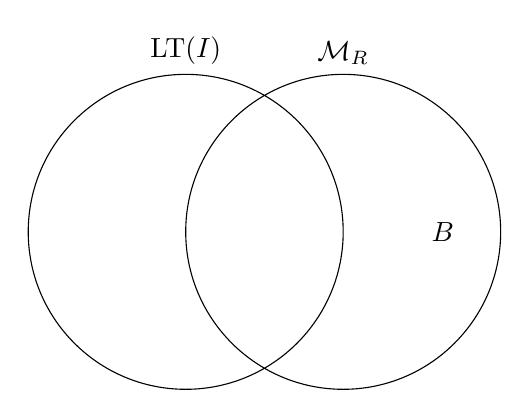
\begin{tikzpicture}
          \draw (-1, 0 ) circle (2)
                (-1, 2 ) node [above] {$\LT(I)$}
                ( 1, 0 ) circle (2)
                ( 1, 2 ) node [above] {$\cal M_R$}
                ( 2, 0 ) node [right] {$B$};
        \end{tikzpicture}
      \end{center}
      
      Either $\LT(f) \in B$ or $\LT(f) \in \LT(I)$.
      In the first case, suppose $\LT(f) = b \in B$.
      Then $f - b \in R - X$ has a smaller leading term than $f$,
      contradicting our choice of $f$.
      Otherwise, suppose $\LT(f) = m \in \LT(I)$.
      Then we can subtract from $f$ any monic polynomial in $I$ with the same leading term,
      again yielding a smaller polynomial in $R - X$.
  \end{description}
\end{proof}

\begin{theorem}
  \label{thm_groebner_basis_product}
  Let $I$ and $J$ be ideals of $R = K[x_1, \ldots, x_n]$, generated by Gr\"obner bases, say
  \begin{align*}
    I &= \pid{f_1, \ldots, f_m} \\
    J &= \pid{g_1, \ldots, g_n}.
  \end{align*}
  Then
  \[ \{ f_ig_j ~|~ 1 \leq i \leq m, 1 \leq j \leq n \} \]
  is a Gr\"obner basis for the ideal product $IJ$.
\end{theorem}
\begin{proof}
  \begin{align*}
    \LT(IJ)
      &= \pid{ \LT(h) ~|~ h \in IJ } \\
      &= \pid{ \LT(fg) ~|~ f \in I, g \in J } \\
      &= \pid{ \LT(f)\LT(g) ~|~ f \in I, g \in J } \\
      &= \pid{ \LT(f) ~|~ f \in I } \pid{ \LT(g) ~|~ g \in J } \\
      &= \LT(I) \LT(J) \\
      &= \pid{ \LT(f_i) ~|~ 1 \leq i \leq m } \pid{ \LT(g_j) ~|~ 1 \leq j \leq n } \\
      &= \pid{ \LT(f_i) \LT(g_j) ~|~ 1 \leq i \leq m, 1 \leq j \leq n } \\
      &= \pid{ \LT(f_i g_j) ~|~ 1 \leq i \leq m, 1 \leq j \leq n }
  \end{align*}
\end{proof}

\begin{theorem}
  \label{thm_groebner_basis_remainder}
  Let $I$ be an ideal of $R$, generated by the Gr\"obner basis $G = \{ g_1, \ldots, g_m \}$. Then
  \begin{enumerate}[label=(\roman*)]
    \item
    Every polynomial $f \in R$ can be written uniquely in the form
    \begin{equation*}
      f = g + r
    \end{equation*}
    where $g \in I$, $r \in R$, and no non-zero term in $r$ is divisible by the leading term of any $g_i$.
    
    \item
    For any polynomial $f \in R$, we have that $f \in I$ if and only if $r = 0$.
  \end{enumerate}
\end{theorem}
\begin{proof}
  \begin{enumerate}[label=(\roman*)]
    \item
    The GPLD algorithm gives $g$ and $r$ satisfying these criteria, demonstrating existence.
    We need only show that these are unique.
    It suffices to show that $r$ is unique, since this uniquely determines $g = f - r$.
    
    Suppose $f = g + r = g' + r'$, with $g, g' \in I$, $r, r' \in R$, and between the non-zero terms of $r$ and $r'$,
    none are divisible by the leading term of any $g_i \in G$.
    Then $r - r' = g' - g \in I$.
    Hence $\LT(r - r') \in \LT(I)$.
    This implies that $\LT(r - r')$ is divisible by some $\LT(g_i)$,
    but this would contradict the fact that no non-zero term in either of $r$ and $r'$ is divisible by any $\LT(g_i)$,
    unless $\LT(r - r') = 0$, whereupon $r = r'$.
    
    \item
    Let $f = g + r$, where $g \in I$ and no non-zero term of $r$ is divisible by any $\LT(g_i)$.

    ($\implies$)
    Suppose $f \in I$.
    Then we can write $f = f + 0$, and this representation is unique by part (i), hence $r = 0$.

    ($\impliedby$)
    Suppose $r = 0$.
    Then $g = g + r = f \in I$.
  \end{enumerate}
\end{proof}

It is an obvious fact that, given any polynomial $f \in K[x_1, \ldots, x_n]$,
we can separate $f$ into its homogeneous components.
That is, we can write
\[ f = \sum_{i = 0}^n f_i^* \]
where $n$ is the total degree of $f$ and $f_i^*$ is homogeneous of degree $i$.

Given a point $P = (a_1, \ldots, a_n) \in \bb A_K^n$, we can even write $f$ in the same form,
but where $f_i^*$ is homogeneous in the variables $(x_1 - a_1), \ldots, (x_n - a_n)$.
E.g., in $\bb Q[x,y]$, given the point $P = (1,1)$, 
\[ x^2 + y^2 = [(x - 1)^2 + (y - 1)^2] + [2(x + 1) + 2(y + 1)] + [2]. \]
This is just the multivariate Taylor series expansion of the polynomial around the point $P$.
This generalizes to the following.

\begin{theorem}
  Let $R = K[x_1, \ldots, x_n]$ and let $I$ be an ideal of $R$ given by a Gr\"obner basis $I = \pid{g_1, \ldots, g_m}$.
  Then $f$ can be written uniquely in the form
  \[ f = \sum_{i=0}^t f_i^*, \]
  where $t = \max\{n \in \bb N ~|~ f \in I^n\}$, $f_i^* \in I^i - I^{i+1}$, and $f_i^* \not\in \LT(I^{i+1})$.
\end{theorem}
\begin{proof}
  By Theorem \ref{thm_groebner_basis_product}, our Gr\"obner basis for $I$ gives us a basis for $I^t$.
  Theorem \ref{thm_groebner_basis_remainder} then applies, allowing us to write
  \[ f = f^*_t + r_t \]
  with $f^*_t \in I^t - I^{t+1}$ and $r_t \in R$, $r_t \not\in \LT(I^t)$.
  Applying Theorems \ref{thm_groebner_basis_product} and \ref{thm_groebner_basis_remainder} $t-1$ more times gives the result.
\end{proof}

Essentially, given finitely polynomials $\{ g_i \}$ forming a Gr\"obner basis for an ideal,
we can uniquely perform a homogenous decomposition of any polynomial $f$ with respect to the $g_i$'s.

This also allows us to show that (over a field of sufficiently large characteristic)
$f \in I^2$ if and only if $f$ and its differential $df$ vanish modulo $I$.
  
%%%%%%%%%%%%%%%%%%%%%%%%%%%
%%%%%                 %%%%%
%%%%%   Derivations   %%%%%
%%%%%                 %%%%%
%%%%%%%%%%%%%%%%%%%%%%%%%%%

\section{Derivations}
\label{chap_differentials}

\begin{definition}
  Let $R$ be a ring, $A$ an $R$-algebra, and $M$ an $A$-module.
  A map $D : A \to M$ is called a \defn{derivation} (from $A$ to $M$) if it is $K$-linear and satisfies the product rule:
    \[ D(ab) = D(a)b + aD(b). \]
\end{definition}

Some authors do not require a derivation to be $R$-linear,
and they distinguish between derivations and $R$-linear derivations.
We will assume all derivations are $R$-linear.

As the name suggest, many familiar properties of the derivative from calculus are an immediate consequence of this definition.

\begin{proposition}
  \label{prop_derivation}
  A derivation satisfies the following properties.
  \begin{enumerate}[label=(\roman*)]
    \item If $A$ is unital, then $D(1) = 0$.
    \item If $A$ is unital, then $D(r) = 0$ for all $r \in R$.
    \item If $A$ is commutative, then $D(x^2) = 2xD(x)$.
    \item If $A$ is commutative, then for all integers $n > 0$, $D(x^n) = nx^{n-1}D(x)$.
    \item If $x$ is a unit, then $D(x\inv) = -x^{-2}D(x)$.
    \item If $x$ is a unit, then for all $n \in \bb Z$, $D(x^n) = nx^{n-1}D(x)$.
    \item If $y$ is a unit, then $D(xy\inv) = (D(x)y - xD(y))y^{-2}$.
  \end{enumerate}
\end{proposition}
\begin{proof}
  \begin{enumerate}[label=(\roman*)]
    \item
      We have
        \[ D(1) = D(1 \cdot 1) = D(1) \cdot 1 + 1 \cdot D(1) = D(1) + D(1) \]
      which implies $D(1) = 0$.
    \item
      Follows from (i) by $R$-linearity.
    \item
        \[ D(x^2) = D(x)x + xD(x) = xD(x) + xD(x) = 2xD(x). \]
    \item
      Follows from (iii) by induction.
      Suppose $D(x^k) = kx^{k-1}D(x)$ for some $k > 0$. Then
      \begin{align*}
        D(x^{k+1})
          &= D(x^k \cdot x) \\
          &= D(x^k)x + x^kD(x) \\
          &= kx^{k-1}D(x)x + x^kD(x) \\
          &= kx^kD(x) + x^kD(x) \\
          &= (k + 1)x^kD(x).
      \end{align*}
    \item
      By part (i) and the product rule, we have
        \[ 0 = D(1) = D(xx\inv) = D(x)x\inv + xD(x\inv). \]
      This implies
        \[ xD(x\inv) = -D(x)x\inv, \]
      hence
        \[ D(x\inv) = -x^{-2}D(x). \]
    \item
      The case where $n \geq -1$ is handled by parts (i), (iv), and (v).
      The rest follows by induction.
      Suppose $D(x^k) = kx^{k-1}D(x)$ for some $k \leq -1$. Then
      \begin{align*}
        D(x^{k-1})
          &= D(x^kx\inv) \\
          &= D(x^k)x\inv + x^kD(x\inv) \\
          &= kx^{k-1}D(x)x\inv - x^kx^{-2}D(x) \\
          &= kx^{k-2}D(x) - x^{k-2}D(x) \\
          &= (k - 1)x^{k-2}D(x).
      \end{align*}
    \item
      Immediate from the product rule and part (v).
      \begin{align*}
        D(xy\inv)
          &= D(x)y\inv + xD(y\inv) \\
          &= D(x)y\inv - xy^{-2}D(y) \\
          &= (D(x)y - xD(y))y^{-2}.
      \end{align*}
  \end{enumerate}
\end{proof}

We can define the sum of two derivations $\delta_1$ and $\delta_2$ by
  \[ (\delta_1 + \delta_2)(x) = \delta_1(x) + \delta_2(x). \]
After we define scalar multiplication
  \[ (k\delta)(x) = k (\delta(x)), \]
the set of derivations from a $R$-algebra $A$ to an $A$-module $A$ becomes an $R$-module,
denoted by $\Der_R(A,M)$.
This is the \defn{module of derivations from $A$ to $M$}.
In the case where $M = A$, this may be denoted by $\Der_R(A)$.

Properties (v), (vi), and (vii) of Proposition \ref{prop_derivation}
show that image of a unit and its inverse under a derivation are interdependent.
This suggests the following.

\begin{proposition}
  \label{prop_derivation_unique_extension}
  Let $D \in \Der_R(A,M)$.
  Let $B = \Frac A$.
  ($A$ is a ring with a $R$-action.
  $\Frac A$ is the field of fractions of the ring $A$ and inherits the $R$-action.)
  There is a unique $D' \in \Der_R(B, M)$ such that $D'|_{D} = D$.
\end{proposition}
That is to say that if $D$ is a derivation from $A$ to $M$,
it extends uniquely to a derivation from $A$'s field of fractions.
\note{Field of fractions requires that $A$ is an integral domain.}
\begin{proof}
  If $A = B$, we are done.
  So suppose instead there is a $b \in B$ such that $b\in A$ but $b\inv \not \in A$.
  Suppose $D', D'' \in \Der_R(B, M)$ are such that $D'|_{D} = D''|_{D} = D$.
  Then $D'(b) = D''(b) = D(b)$ and
    \[ D'(b\inv) = -b^{-2}D'(b) = -b^{-2}D''(b) = D''(b\inv). \]
  It follows that $D'(ab\inv) = D''(ab\inv)$ for all $ab\inv \in B$.
\end{proof}

In order to understand how a derivation acts on $\Frac A$, it is enough to know how it acts on $A$.
In the case of a derivation over the field $R(x_1, \ldots, x_n)$,
it is enough to know how it acts on the polynomial ring $R[x_1, \ldots, x_n]$.
In the univariate case, we can say even more.
The behaviour of a derivation $D: R(x) \to M$ is entirely determined by the value of $D(x)$.

\begin{proposition}
  \label{prop_derivation_unique_x}
  Let $R(x)$ be the ring of rational functions over a ring $R$ in a single variable $x$.
  Let $\delta, \eta \in \Der_R(R(x))$.
  If $\delta(x) = \eta(x)$, then $\delta = \eta$.
\end{proposition}
\begin{proof}
  For all $r \in R$, we have $\delta(r) = \eta(r) = 0$.
  For all $f \in R[x]$, we have $\delta(f) = \eta(f)$ by $R$-linearity.
  Now $\delta$ and $\eta$ agree on all of $R[x]$.
  By Proposition \ref{prop_derivation_unique_extension}, they must agree on all of $R(x)$.
\end{proof}

Up to this point, we have discussed derivations without showing that such a thing even exists.
The following proposition establishes the existence of derivations by exhibiting one that should be familiar.

\begin{proposition}
  \label{prop_derivation_formal_derivative}
  Let $R(x)$ be the ring of rational functions over a ring $R$ in a single variable $x$.
  There is a unique derivation $D_x : R(x) \to R(x)$ satisfying $D_x(x) = 1$.
\end{proposition}
Given a rational function $f(x)$, the function $D_x(f(x))$ is the \defn{formal derivative} of $f(x)$, often written $f'(x)$.
\begin{proof}
  We need only show existence of a derivation on $R[x]$ with the desired property.
  By propositions \ref{prop_derivation_unique_extension} and \ref{prop_derivation_unique_x},
  this derivation is unique and extends uniquely to a derivation on $R(x)$ with the desired property.
  
  We set $D_x(x) = 1$ and extend by linearity to get its action on all of $R[x]$.
  If $f(x) = \sum f_ix^i \in R[x]$, then
    \[ D(f(x)) = \sum if_ix^{i-1}D(x) = \sum if_ix^{i-1}. \]
  We must show that this satisfies the product rule.
  Let $g(x) = \sum g_jx^j$. Then for all $f(x), g(x) \in R[x]$,
  
  \begin{align*}
    D_x(f(x)g(x))
      &= D_x \left( \left( \sum_{i=0}^m f_ix^i \right) \left( \sum_{j=0}^n g_jx^j \right) \right) \\
      &= D_x \left( \sum_{i=0}^m \sum_{j=0}^n f_ix^i g_jx^j \right) \\
      &= D_x \left( \sum_{i=0}^m \sum_{j=0}^n f_ig_jx^{i+j} \right) \\
      &= \sum_{i=0}^m \sum_{j=0}^n f_ig_jD_x(x^{i+j}) \\
      &= \sum_{i=0}^m \sum_{j=0}^n (i+j)f_ig_jx^{i+j-1} \\
      &= \sum_{i=0}^m \sum_{j=0}^n (if_ig_jx^{i+j-1} + jf_ig_jx^{i+j-1}) \\
      &= \sum_{i=0}^m \sum_{j=0}^n if_ig_jx^{i+j-1} + \sum_{i=0}^m \sum_{j=0}^n jf_ig_jx^{i+j-1} \\
      &= \left( \sum_{i=0}^m if_ix^{i-1} \right) \left( \sum_{j=0}^n g_jx^j \right) + \left( \sum_{i=0}^m f_ix^i \right) \left( \sum_{j=0}^n jg_jx^{j-1} \right) \\
      &= D_x(f(x)) g(x) + f(x)D(g(x)).
  \end{align*}
\end{proof}
\begin{example}
  Let $f(x) = 3x^3 + 6x^2 + 1 \in \bb Z[x]$. Then
  \begin{align*}
    D_x(f(x))
      &= 3D_x(x^3) + 6D_x(x^2) + D_x(1) \\
      &= 3 \cdot 3 x^2 D_x(x) + 6 \cdot 2 x D_x(x) + 0 \\
      &= 9 x^2 + 12 x. \\
  \end{align*}
\end{example}

Now consider the $R$-algebra $A = R(x_1, \ldots, x_n)$.
For any fixed $1 \leq t \leq r$, we can set $S = R(x_1, \ldots, x_{t-1}, x_{t+1}, \ldots, x_n)$
so that $A = S(x_t)$.
Then there is a unique derivation $D_{x_t} \in \Der_S(A,M)$ satisfying $D_{x_t}(x_t) = 1$.
This derivation is also a member of $\Der_R(A,M)$.
For any $f \in A$, the function $D_{x_t}(f)$ is the \defn{formal partial derivative} of $f$, often written $f_{x_t}$.
This is the unique derivation with the properties
\begin{align*}
  D_{x_t}(x_k) &= \begin{cases} 1 & k = t \\ 0 & k \neq t \end{cases}.
\end{align*}
\begin{example}
  In the case of $A = \bb Z[x,y]$, we have derivations $D_x$ and $D_y$ with
  $D_x(x) = 1$, $D_x(y) = 0$, $D_y(x) = 0$, and $D_y(y) = 1$.
  Let $f(x,y) = x^2 + xy + y^3 \in \bb Z[x,y]$.
  Then $D_x(f) = 2x + y$ and $D_y(f) = x + 3y^2$.
\end{example}

\begin{proposition}
  Let $D \in \Der_K(A)$ be a derivation.
  Let $I$ be an ideal of $A$.
  Then $D$ induces a derivation $D^* \in \Der_K(A/I)$ defined by
    \[ D^*([a]) = [D(a)]. \]
\end{proposition}
\begin{proof}
  For each $a \in A$, denote the equivalence class containing $a$ in $A/I$ by $\bar a$.
  We show first that this map is well-defined.
  Suppose $\bar a = \bar b$.
  Then $\bar{a-b} = \bar 0$ and
    \[ D^*(\bar a) = D^*(\bar a - \bar{a-b}) = D^*(\bar{a-a+b}) = D^*(\bar b). \]
  We must also show that $D^*(\bar k \cdot \bar a) = \bar k \cdot D^*(\bar a)$
  and $D^*(\bar a \cdot \bar b) = D^*(\bar a) \cdot \bar b + \bar a \cdot D^*(\bar b)$.
    \[ D^*(\bar k \cdot \bar a) = D^*(\bar{ka}) = \bar{D(ka)} = \bar{kD(a)} = \bar k \cdot \bar{D(a)} = \bar k \cdot D^*(\bar a) \]
  \begin{align*}
    D^*(\bar a \cdot \bar b)
      &= D^*(\bar{ab})
       = \bar{D(ab)}
       = \bar{D(a)b + aD(b)} \\
       &= \bar{D(a)} \cdot \bar b + \bar a \cdot \bar{D(b)}
       = D^*(\bar a) \cdot \bar b + \bar a \cdot D^*(\bar b)
  \end{align*}
\end{proof}
With this we can extend formal derivatives of functions in $K[x,y]$ and $K(x,y)$ to formal derivatives of functions in $K[C]$ and $K(C)$.

\begin{proposition}
  \label{prop_precompose_derivation}
  Let $f \in \Hom_R(A,B)$ be a morphism of $R$-algebras and let $D \in \Der_R(B,M)$ be an $R$-linear derivation.
  \[ \begin{tikzcd} A \arrow{r}{f} & B \arrow{r}{D} & M \end{tikzcd} \]
  Then $D \circ f \in \Der_R(A,M)$.
\end{proposition}
\begin{proof}
  While $M$ is a $B$-module, it becomes an $A$-module under the $A$-action
    \[ A \times M \to M : (a, m) \mapsto f(a)m. \]
  Both $f$ and $D$ are $R$-linear, so $D \circ f$ is also $R$-linear.
  As for the product rule, let $a, b \in A$. Then
  \begin{align*}
    (D \circ f)(ab)
      &= D(f(ab)) \\
      &= D(f(a)f(b)) \\
      &= D(f(a))f(b) + f(a)D(f(b)) \\
      &= (D \circ f(a))f(b) + f(a)(D \circ f(b)) \\
      &= (b, D \circ f(a)) + (a, D \circ f(b)).
  \end{align*}
\end{proof}


%%%%%%%%%%%%%%%%%%%%%%%%%%%%%%%%%%%%
%%%%%                          %%%%%
%%%%%   Universal Derivation   %%%%%
%%%%%                          %%%%%
%%%%%%%%%%%%%%%%%%%%%%%%%%%%%%%%%%%%

\subsection{Universal Derivation}

\note{Notes based on Eisenbud's Commutative Algebra with a View Towards Algebraic Geometry.}

\begin{itemize}
  \item Module of Kahler Differentials $\Omega$
  \item Universal Derivation mapping algebra to $\Omega$
  \item Local properties of $\Omega$
  \item $\Omega$ can be realized locally as $m/m^2$.
\end{itemize}

\begin{definition}
  Let $A$ be an $R$-algebra.
  The \defn{module of K\"ahler differentials} of $A$ over $R$,
  denoted by $\Omega_{A/R}$,
  is the $A$-module generated by the set $\{ d(a) ~|~ a \in A \}$
  modulo the relations
  \begin{align*}
    d(ab) &= d(a)b + ad(b) \\
    d(ra + sb) &= rd(a) + sd(b)
  \end{align*}
  for all $r, s \in R$ and $a, b \in A$.
\end{definition}

\begin{definition}
  The map
    \[ d : A \to \Omega_{A/R} : a \mapsto d(a) \]
  is an $R$-linear derivation, called the \defn{universal derivation}.
\end{definition}

It is universal in the following sense.
If $e : A \to M$ is another $R$-linear derivation,
then there is a unique morphism of $R$-modules $e' : \Omega_{A/R} \to M$ such that
\[ \begin{tikzcd}
  A \arrow{r}{d} \arrow[swap]{dr}{e} & \Omega_{A/R} \arrow[dashed]{d}{!\exists e'} \\ & M
\end{tikzcd} \]
commutes.
This map is defined by $e' : da \mapsto e(a)$.

\begin{proposition}
  A morphism $f : A \to B$ of $R$-algebras induces a map $\Omega_{A/R} \to \Omega_{B/R}$.
\end{proposition}
\begin{proof}
  We have the following maps,
  \[ \begin{tikzcd}
      A \arrow{r}{d} \arrow[swap]{d}{f} & \Omega_{A/R} \\ B \arrow[swap]{r}{d'} & \Omega_{B/R}.
    \end{tikzcd} \]
  By Proposition \ref{prop_precompose_derivation}, the composition $d' \circ f : A \to \Omega_{B/R}$ is an $R$-linear derivation.
  By the universal property of the universal derivation, there is a unique map $f' : \Omega_{A/R} \to \Omega_{B/R}$.
  \[ \begin{tikzcd}
      A \arrow{r}{d} \arrow[swap]{dr}{d' \circ f} & \Omega_{A/R} \arrow[dashed]{d}{} \\ & \Omega_{B/R}
    \end{tikzcd} \]
\end{proof}
The induced map sends $da \mapsto d'(f(a))$.

\begin{proposition}
  Let $A = R[x_1, \ldots, x_n]$. Then
  \[ \Omega_{A/R} \cong \bigoplus_{i=1}^n Adx_i. \]
\end{proposition}
\begin{corollary}
  Let $A = R[x_1, \ldots, x_n]$, let $I$ be an ideal of $A$, and let $B = A/I$.
  Then $B$ is an $R$-algebra and
  \[ B \otimes_{R} \Omega_{A/R} \cong \bigoplus_{i=1}^n Bdx_i. \]
\end{corollary}
\begin{proof}
  \note{Extension of scalars.}
\end{proof}

Since $\Omega_{A/R}$ is a direct sum of $R$-algebras $Adx_i$,
there is a family of natural projection maps 
  \[ \pi_i : \Omega_{A/R} \to Adx_i : \sum f_jdx_j \mapsto f_idx_i. \]
We can compose the maps
  \[ \begin{tikzcd}
    A \arrow{r}{d} & \Omega_{A/R} \arrow{r}{\pi_i} & Adx_i \arrow{r}{} & A
  \end{tikzcd} \]
where the right-most map sends $dx_i \mapsto 1$.
The composition of the three maps is the formal partial derivative with respect to $x_i$.

\begin{proposition}
  \label{prop_exact_sequence_cokernel}
  If $A \xrightarrow f B \xrightarrow g C \to 0$ is an exact sequence, then
    \[ C \cong \coker f = B / \im f = B / \ker g = \coim g. \]
\end{proposition}
\begin{proof}
  \note{Hungerford, p.176}
\end{proof}

\begin{proposition}
  \label{prop_conormal_sequence}
  Let $\pi : A \to B$ is an epimorphism of $R$-algebras.
  Let $I = \ker \pi$.
  There is an exact sequence of $B$-modules
    \[ I/I^2 \xrightarrow{d} B \tensor A \Omega_{A/R} \xrightarrow{D\pi} \Omega_{B/R} \to 0 \]
  where $d : [f] \mapsto 1 \otimes df$ and $D\pi : b \otimes da \mapsto b(da)$.
\end{proposition}
\begin{proof}
  \note{Eisenbud, CAwaVtAG, Prop. 16.3.}
\end{proof}

We can apply Proposition \ref{prop_conormal_sequence} in the following way.
Let $A = K[x,y]$.
Let $C$ be a $C_{3,4}$ curve defined by the polynomial $f$.
Then $\pi : A \mapsto K[C]$ is an epimorphism with kernel $\pid f$.
We can compute the image of the map
  \[ d : \frac{\pid f}{\pid{f^2}} \to K[C] \tensor A \Omega_{A/R}. \]
Let $[gf]$ be an arbitrary element of $\pid f / \pid{f^2}$. Then
\begin{align*}
  d(gf)
    &= 1 \tensor A d(gf) \\
    &= 1 \tensor A (d(g)f + gd(f)) \\
    &= 1 \tensor A d(g)f + 1 \tensor A gd(f) \\
    &= f \tensor A d(g) + g \tensor A d(f) \\
    &= 0 \tensor A d(g) + g \tensor A d(f)
      & f \equiv 0 \text{ in } K[C] \\
    &= g \tensor A df
\end{align*}
We have also that $K[C] \tensor A \Omega_{A/R} = K[C]dx \oplus K[C]dy$, since
\begin{align*}
  K[C] \tensor A \Omega_{A/R}
    &= K[C] \tensor A \left( Adx \oplus Ady \right) \\
    &= \left( K[C] \tensor A Adx \right) \oplus \left( K[C] \tensor A Ady \right) \\
    &= K[C]dx \oplus K[C]dy.
\end{align*}
The element $1 \otimes df \in K[C] \otimes \Omega_{A/R}$ corresponds to $f_xdx + f_ydy \in K[C]dx \oplus K[C]dy$.
Applying Propositions \ref{prop_exact_sequence_cokernel} and \ref{prop_conormal_sequence},
we have that
  \[ \Omega_{K[C]/K} = \frac {K[C] \tensor A \Omega_{A/R}} {\im d} = \frac {K[C]dx \oplus K[C]dy} {\im d}, \]
which is the free $K[C]$-algebra generated by $dx$ and $dy$, modulo the relation $f_xdx + f_ydy = 0$.
\note{(Double check this.)}






\subsection{Unsorted Stuff}

\begin{theorem}
  Let $A = K[x_1, \ldots, x_n]$ and let $I$ be an ideal of $A$.
  If $f \in I^2$, then $f \equiv 0$ and $df \equiv 0$ modulo $I$.
\end{theorem}
\begin{proof}
  Let $f \in I^2$.
  Then $f \in I$, so $f \equiv 0 \pmod I$.
  As for its differential, we have that $f$ is generated by a Gr\"obner basis {$g_i$}
  \[ f = \sum a_{i,j}g_ig_j, \]
  so
  \begin{align*}
    df &= d \left( \sum_{\substack{1 \leq i \leq j \leq m}} a_{i,j}g_ig_j \right) \\
       &= \sum_{\substack{1 \leq i \leq j \leq m}} d \left( a_{i,j}g_ig_j \right) \\
       &= \sum_{\substack{1 \leq i \leq j \leq m}} \left( d(a_{i,j})g_ig_j + a_{i,j}d(g_i)g_j + a_{i,j}g_id(g_j) \right) \\
       &\equiv 0 \pmod I
  \end{align*}
\end{proof}

The converse is not true in general.
A simple counterexample is to let $A = \bb F_2[x]$, let $f = x^2$, and let $I = \pid f$.
Then $f \equiv 0 \pmod I$ and $df = 2xdx \equiv 0 \pmod I$.
However, $f \not\in I^2 = \pid{x^4}$.

It is true under additional assumptions.

\begin{theorem}
  Let $A = K[x_1, \ldots, x_n]$ and let $I$ be an ideal of $A$.
  Let $f \in A$ be a polynomial whose formal partial derivatives do not all vanish.
  If $f, df \equiv 0 \pmod I$, then $f \in I^2$.
\end{theorem}
\begin{proof}
  We prove the contrapositive.
  Suppose $f \not\in I^2$.
  If $f \not\equiv 0 \pmod I$, we are done, so suppose $f \equiv 0 \pmod I$ (i.e. $f \in I$).
  We wish to show that $df \not\equiv 0 \pmod I$.

  By Theorem \ref{thm_groebner_basis_remainder}, we can write $f$ as
  \[ f = g + r \]
  where $g \in I^2$ and $r \not\in \LT(I^2)$. Furthermore, $0 \neq r \in I$.
  Since $r \not\in \LT(I^2)$, $D_{x_k}(r) \not\in \LT(I^2)$ for any $1 \leq k \leq n$.
  \begin{align*}
    df &= dg + dr \\
       &\equiv dr \pmod I \\
       &= \sum D_{x_i}(r)dx_i
  \end{align*}
  We must argue now that for each summand $D_{x_i}(r)dx_i$ is non-zero modulo $I$.
  
  Suppose that $D_{x_k}(r) \equiv 0$ for some $1 \leq k \leq n$.
  \begin{align*}
    & D_{x_k}(r) \equiv 0 \pmod I \\
    \implies & D_{x_k}(r) \in I \\
    \implies & \LT(D_{x_k}(r)) \in \LT(I) \\
    \implies & \LT(D_{x_k}(r)) \in \LT(I)\LT(I) \\
    \implies & \LT(D_{x_k}(r)) \in \LT(I^2).
  \end{align*}
  However, as noted earlier, no term in $D_{x_k}(r)$ is in $\LT(I^2)$.
  \note{(Wording.)}
\end{proof}

\begin{proof}
  We prove the contrapositive.
  Suppose $f \not\in I^2$.
  If $f \not\equiv 0 \pmod I$, we are done, so suppose $f \equiv 0 \pmod I$ (i.e. $f \in I$).
  We wish to show that $df \not\equiv 0 \pmod I$.

  By Theorem \ref{thm_groebner_basis_remainder}, we can write $f$ as
  \[ f = g + r \]
  where $g \in I^2$ and $r \not\in \LT(I^2)$.
  Taking the differential of $f$,
  \begin{align*}
    df &= \sum_{i=1}^n D_{x_i}(f)dx_i.% \\
%       &= \sum_{i=1}^n D_{x_i}(g + r)dx_i \\
  \end{align*}
  We must show that one of $df$'s summands is non-zero modulo $I$.
  Since $f$ has a non-zero formal partial derivative, let $k$ be such that $D_{x_k}(f) \neq 0$.
  Then
  \begin{align*}
    D_{x_k}(f)
      &= D_{x_k}(g + r) \\
      &= D_{x_k}(g) + D_{x_k}(r) \\
      &\equiv D_{x_k}(r) \pmod I.
  \end{align*}
  Now suppose $D_{x_k}(r) \equiv 0 \pmod I$. Then
  \begin{align*}
    & D_{x_k}(r) \equiv 0 \pmod I \\
    \implies & D_{x_k}(r) \in I \\
    \implies & \LT(D_{x_k}(r)) \in \LT(I) \\
    \implies & \LT(D_{x_k}(r)) \in \LT(I)\LT(I) \\
    \implies & \LT(D_{x_k}(r)) \in \LT(I^2).
  \end{align*}
  %However, as noted earlier, no term in $D_{x_k}(r)$ is in $\LT(I^2)$.
  %\note{(Wording.)}
\end{proof}

\begin{proof}
  \note{(Supposing $I = \sqrt I$.)}
  We prove the contrapositive.
  Suppose $f \not\in I^2$.
  If $f \not\equiv 0 \pmod I$, we are done, so suppose $f \equiv 0 \pmod I$ (i.e. $f \in I$).
  We wish to show that $df \not\equiv 0 \pmod I$.

  By Theorem \ref{thm_groebner_basis_remainder}, we can write $f$ as
  \[ f = g + r \]
  where $g \in I^2$ and $r \not\in \LT(I^2)$.
  Taking the differential of $f$,
  \begin{align*}
    df &= dg + dr \\
       &\equiv dr \pmod I \\
       &= d\left(\sum_{i=1}^m a_ig_i \right) \\
       &\equiv \sum_{i=1}^m a_id(g_i) \pmod I.
  \end{align*}
\end{proof}

%%%%%%%%%%%%%%%%%%%%%%%%%
%%%%%              %%%%%
%%%%%   Divisors   %%%%%
%%%%%              %%%%%
%%%%%%%%%%%%%%%%%%%%%%%%

\section{Divisors}
\subsection{The Divisor Class Group}

Let $C$ be a non-singular, projective curve over a field $K$.
The \defn{group of divisors} on $C$, denoted by $\Div_{\bar K}(C)$, is the free Abelian group generated by the points of $C(\bar K)$.
A \defn{divisor} of $C$ is any element of this group; it is a finite formal sum of points.
If $P$, $Q$, and $R$ are points on the curve $C$, then examples of divisors include
  \[ \begin{array}{c} P + Q + R \\ P + 3Q - 2R \\ Q \\ 0 \end{array}. \]

If $D$ is a divisor and $P$ is a point on $C$, the \defn{order} of $D$ at $P$, denoted by $\ord_P(D)$, is the coefficient of $P$ in this sum.
For example, if $D = P + 3Q - 2R$, then $\ord_Q(D) = 3$ and $\ord_R(D) = -2$.
A divisor $D$ is called \defn{effective} if $\ord_P(D) \geq 0$ at every point $P$.
So $P + Q + R$, $Q$, and $0$ are effective divisors, while $P + 3Q - 2R$ is not.

The degree of a divisor, denoted by $\deg(D)$, is the sum of the orders of $D$ at all points,
  \[ \deg(D) = \sum_{P \in C}\ord_P(D). \]
For instance, $\deg(P + 3Q - 2R) = 2$.
If $D$ and $D'$ are both divisors of $C$, then $\deg(D + D') = \deg(D) + \deg(D')$.
Consequently, divisors with degree zero form a subgroup $\Div_{\bar K}^0(C)$ of $\Div_{\bar K}(C)$.

If $L$ is an algebraic extension of $K$ and $\sigma \in \Gal(\bar K/L)$,
then $\sigma$ extends an action on points of $C(L)$, via
  \[ \sigma(x : y : z) = (\sigma(x) : \sigma(y) : \sigma(z)). \]
This, in turn, extends to an action on $\Div_{\bar K}(C)$.
If $D$ is the divisor
  \[ D = \sum_{P \in C(\bar K)} n_P P, \]
then define
  \[ \sigma(D) = \sum_{P \in C(\bar K)} n_P \sigma(P). \]
A divisor $D$ is \defn{defined over $L$} if $\sigma(D) = D$ for all $\sigma \in \Gal(\bar K/L)$.
That is, if $D$ remains fixed by every embedding of $L$ in $\bar K$.
The set of divisors on $C$ defined over $L$ is denoted by $\Div_L(C)$.
The set $\Div_L(C)$ forms a subgroup of $\Div_{\bar K}(C)$, and $\Div_L^0(C)$ a subgroup of both $\Div_L(C)$ and $\Div_{\bar K}^0(C)$.

This last definition deserves a few examples.
\begin{example}
  Let $K$ be any field, $L$ any algebraic extension and $\sigma \in \Gal(\bar K/L)$.
  By definition, $\sigma$ fixes $L$.
  If $P$ is any point with coordinates in $L$, then $\sigma(P) = P$.
  If $D$ is any divisor consisting only of points with coordinates in $L$, then $\sigma(D) = D$ and $D$ is defined over $L$.
\end{example}
\begin{example}
  Let $K = \bb F_2$ and let $L = K(\alpha)$ be an algebraic extension with $\alpha^2 + \alpha = 1$.
  Let $C$ be the curve $x^4 + y^3 + x + 1$ over $K$.
  Let $P$ be the point $(\alpha : 1 : 1)$ on $C$ and let $D$ be the divisor $D = P$.
  There is an automorphism $\sigma \in \Gal(\bar K/K)$ that maps $\alpha \mapsto \alpha + 1$, so 
    \[ \sigma(D) = \sigma(P) = (\sigma(\alpha) : \sigma(1) : \sigma(1)) = (\alpha + 1 : 1 : 1) \neq D. \]
  Hence $D$ is not defined over $K$.
\end{example}
\begin{example}
  Let $K$, $L$, $C$, and $P$ be as in the previous example.
  Let $Q = (\alpha + 1 : 1 : 1)$, which is also a point on $C$.
  Let $D$ be the divisor $D = P + Q$.
  Every automorphism $\sigma$ in $\Gal(\bar K/K)$ maps either $\alpha$ to itself or to $\alpha + 1$.
  In the former case,
  \begin{align*}
    \sigma(D) &= \sigma(P) + \sigma(Q) \\
              &= (\sigma(\alpha) : \sigma(1) : \sigma(1)) + (\sigma(\alpha + 1) : \sigma(1) : \sigma(1)) \\
              &= (\alpha : 1 : 1) + (\alpha + 1 : 1 : 1) \\
              &= P + Q = D.
  \end{align*}
  In the latter case,
  \begin{align*}
    \sigma(D) &= \sigma(P) + \sigma(Q) \\
              &= (\sigma(\alpha) : \sigma(1) : \sigma(1)) + (\sigma(\alpha + 1) : \sigma(1) : \sigma(1)) \\
              &= (\alpha + 1 : 1 : 1) + (\alpha : 1 : 1) \\
              &= Q + P = D.
  \end{align*}
  So $D$ is defined over $K$.
\end{example}

A divisor, being a formal sum of points, can be used to record the zeroes and poles of a function.
Let $f \in K(C)$ be a rational function.
The \defn{divisor of $f$} is
  \[ \div f := \sum_{P \in C(\bar K)} v_P(f)P, \]
where $v_P(f)$ is the valuation of $f$ at $P$ (with respect to the curve $C$).
Recall \note{(from an earlier section)} that $v_P(f)$ is the multiplicity of the intersection of $f$ and $C$ at $P$.
\note{(What if $v_P(f) < 0$?)}
If $D$ is the divisor of some rational function, then $D$ is called a \defn{principal divisor}.
In the following, we will see that principal divisors form a subgroup of degree zero divisors.

\begin{proposition}
  Let $k \in K^*$ and let $f, g \in K(C)^*$. Then
  \begin{enumerate}[label=(\roman*)]
    \item $\div(k) = 0$;
    \item $\div(fg) = \div f + \div g$.
  \end{enumerate}
\end{proposition}
\begin{proof}
  \note{TODO}
\end{proof}
\begin{theorem}
  Let $C$ be a curve over $K$ and let $f \in K(C)^*$.
  Then $f$ has finitely many zeroes and poles and $\deg(\div f) = 0$.
\end{theorem}
\begin{proof}
  Galbraith Thm 8.3.14.
\end{proof}

These theorems combined show that the principal divisors are a subset of the degree zero divisors and remain closed as a group.
They therefore form a (normal) subgroup of $\Div_{\bar K}^0(C)$.
The group of principal divisors on $C$ (defined over $K$) is denoted by $\Princ_K(C)$.

At last we arrive at defining the divisor class group.
The \defn{divisor class group} is the quotient group,
  \[ \Jac_K^0(C) = \frac{\Div_K^0(C)}{\Princ_K(C)}. \]
The divisor class group of $C$ is also called the \defn{Jacobian} of $C$ or the \defn{Picard group} of $C$.
It is sometimes denoted by $\Pic_K^0(C)$.

\begin{itemize}
  \item Every divisor equivalent to one of the form $P_1 + \dots + P_n - nP_\infty$.
        (For any term of the form $-mP$, add $m \div f$ for any polynomial $f$ through $P$.)
  \item Riemann Roch Theorem implies divisor equivalent to one with $n \leq g$. (How?)
        Such a divisor is called reduced. (Is it unique?)
\end{itemize}

Operations with divisors.
\begin{itemize}
  \item Addition
  \item Negation
  \item LCM
  \item GCD
\end{itemize}



\subsection{The Ideal Class Group}

Given the point set of a curve, we were able to construct the divisor class group of the curve.
For a ring (more specifically, a Dedekind domain), there is an analogous construction -- the ideal class group of the ring.

Given a ring $R$, there are several binary operations on the set of ideals of $R$.
Among them is multiplication, and the ring $R$ is an identity element under this operation.
The ideals of $R$ therefore form a monoid under multiplication.
The \emph{fractional} ideals of $R$ form a group.

A \defn{fractional ideal} of $R$ is an $R$-submodule $I$ of the field of fractions $\Frac(R)$
such that there is an element $r \in R$ making $rI \subseteq R$.
The principal fractional ideals of $R$ form a subgroup of the fractional ideals.
If $\pid {a/b}$ is a principal fractional ideal, then $b\pid{a/b} = \pid a \subseteq R$.
The \defn{ideal class group} is the group quotient of the fractional ideals by the principal fractional ideals.
Thus, it induces an equivalence relation on fractional ideals.
Two fractional ideals $I$ and $J$ are equivalent if $IJ\inv$ is principal.
We can rephrase this slightly.
Fractional ideals $I$ and $J$ are equivalent if there are elements $a, b$ in $R$ such that $aI = bJ$.
  \[ I \equiv J \iff \exists \frac a b \in \Frac(R) : IJ\inv = \pid{\frac a b} \iff \exists a, b \in R : aI = bJ. \]

In the ideal class group, every fractional ideal is equivalent to an integral ideal. \note{(Define integral.)}
After all, if $I$ is fractional, then there is an $r \in R$ such that $rI \subseteq R$.
But $J = rI$ is an $R$-submodule of $\Frac (R)$ contained in $R$, so it is an $R$-submodule of $R$, i.e. an ideal of $R$.
Since $rI = 1J$, we have $I \equiv J$.
Since every fractional ideal is equivalent to an integral ideal, when working in the ideal class group,
we can get away with working entirely with integral ideals.
(We will see later how to find an integral ideal equivalent to $I\inv$.)

An important fact for this thesis is the following.
\begin{theorem}
  The divisor class group $\Div_K^0(C)$ of a curve $C$ is isomorphic to the ideal class group of its coordinate ring, $K[C]$:
    \[ \Jac_K(C) \cong \Cl(K[C]). \]
\end{theorem}
Divisors defined over $K$ may consist of points lying in an algebraic extension of $K$.
Because of this, performing operations on the points themselves can be computationally expensive.
By operating in the ideal class group instead, we can do all of our computations over the base field $K$.
To prove this theorem, we will demonstrate an isomorphism between the groups.

\begin{theorem}
  Let $\Id(K[C])$ denote the group of fractional ideals of $K[C]$ and define the maps
  \begin{align*}
    \div(-) : \Id(K[C]) &\to \Div_K^0(C) \\
    I &\mapsto \sum_{P \in C} \min_{f \in I}\{v_P(f)\}P
  \end{align*}
  and
  \begin{align*}
    I_{(-)} : \Div_K^0(C) &\to \Id(K[C]) \\
    D &\mapsto \{ f \in K(C)^* ~|~ \forall P \in C : v_P(f) \geq \ord_P(D) \}.
  \end{align*}
  Then $\div(-)$ is an isomorphism of groups and $I_{(-)}$ is its inverse.
\end{theorem}
\begin{lemma}
  If $I$ is a fractional ideal of $K[C]$, then $\div I$ is a degree zero divisor on $C$ defined over $K$.
\end{lemma}
\begin{proof}
  $\div I = \sum_{P \in C} \min_{f \in I}\{v_P(f)\}P$.
\end{proof}
\begin{lemma}
  If $D$ is a degree zero divisor on $C$ defined over $K$,
  then $I_D$ is a fractional ideal of $K[C]$.
\end{lemma}
\begin{proof}
\end{proof}
\begin{lemma}
  $I_{\div I} = I$.
\end{lemma}
\begin{proof}
\end{proof}
\begin{lemma}
  $\div(I_D) = D$.
\end{lemma}
\begin{proof}
\end{proof}
\begin{lemma}
  $\div(IJ) = \div(I) + \div(J)$.
\end{lemma}
\begin{proof}
\end{proof}

Let $[D]$ be a divisor class and assume that $D$ is a reduced divisor, since $[D]$ has such a representative.
Then
  \[ D = P_1 + \dots + P_r - rP_\infty, \]
where $r \leq g$ \note{(define $g$)} and the $P_i$'s are affine, but not necessarily distinct.
Define $I_D$ to be the ideal
  \[ I_D := \{ f \in K[C] ~|~ \forall P \in C : v_P(f) \geq \ord_P(D) \}. \]
In words, the divisor $D$ encodes a bunch of points on $C$ (possibly with multiplicity greater than one)
and $I_D$ is the ideal consisting of all polynomials that intersect $C$ at those points with at least the prescribed multiplicities.

In the other direction, suppose $I$ is an ideal of $K[C]$.
Define $\div(I)$ to be the divisor
  \[ \div(I) = \sum_{P \in C} \min\{ v_P(f) ~|~ f \in I \}P. \]
\note{(As defined, this is not a degree-zero divisor.)}
The divisor $\div(I)$ consists of all points on $C$ at which every polynomial in $I$ vanishes.
If all polynomials in $I$ vanish at a point with multiplicity greater than 1,
then the order of $\div(I)$ at that point is smallest multiplicity with which any of them vanish.

\note{I will need to show this is well-defined. It may be easier not to assume $D$ is effective/reduced.}
  \[ I_D := \{ f \in K(C) ~|~ \forall P \in C : v_P(f) \geq \ord_P(D) \}. \]
  \[ \div(I) = \sum_{P \in C} \min\{ v_P(f) ~|~ f \in I \}P. \]
Need to show $\div(I_D) = D$ and $I_{\div I} = I$.

\begin{itemize}
  \item Divisor represented by ideal of polynomials through points.
  \item Divisor defined over K given by polynomials over K.
\end{itemize}




\subsection{Types of Divisors}

\begin{comment}
\begin{center}
\begin{tabular}{l|l|l}
% DEGREE | TYPE | POLYS
  Degree & Type & Basis \\
  \hline
  0 & 0 & $1$ \\
  \hline
  \multirow{2}{*}{1}
    &\multirow{2}{*}{11}
      & $x + f_0$, \\
    & & $y + g_0$ \\
  \hline
  \multirow{4}{*}{2}
    &\multirow{2}{*}{21}
      & $y + f_1x + f_0$, \\
    & & $x^2 + g_1x + g_0$ \\
    \cline{2-3}
    &\multirow{2}{*}{22}
      & $x + f_0$, \\
    & & $y^2 + g_2y + g_0$ \\
  \hline
  \multirow{6}{*}{3}
    &\multirow{3}{*}{31}
      & $x^2 + f_2y + f_1x + f_0$, \\
    & & $xy + g_2y + g_1x + g_0$, \\
    & & $y^2 + h_2y + h_1x + h_0$ \\
    \cline{2-3}
    &\multirow{2}{*}{32}
      & $y + f_1x + f_0$, \\
    & & $x^3 + g_3x^2 + g_1x + g_0$ \\
    \cline{2-3}
    &\multirow{1}{*}{33}
      & $x + f_0$ \\
  \hline
  \multirow{8}{*}{4}
    &\multirow{3}{*}{41}
      & $xy + f_3x^2 + f_2y + f_1x + f_0$, \\
    & & $y^2 + g_3x^2 + g_2y + g_1x + g_0$, \\
    & & $x^3 + h_3x^2 + h_2y + h_1x + h_0$ \\
    \cline{2-3}
    &\multirow{2}{*}{42}
      & $x^2 + f_2y + f_1x + f_0$, \\
    & & $xy + g_2y + g_1x + g_0$ \\
    \cline{2-3}
    &\multirow{2}{*}{43}
      & $x^2 + f_2y + f_1x + f_0$, \\
    & & $y^2 + g_4xy + g_2y + g_1x + g_0$ \\
    \cline{2-3}
    &\multirow{1}{*}{44}
      & $y + f_1x + f_0$
  \hline
  \multirow{9}{*}{5}
    &\multirow{3}{*}{51}
      & $y^2 + f_4xy + f_3x^2 + f_2y + f_1x + f_0$, \\
    & & $x^3 + g_4xy + g_3x^2 + g_2y + g_1x + g_0$, \\
    & & $x^2y + h_4xy + h_3x^2 + h_2y + h_1x + h_0$ \\
    \cline{2-3}
    &\multirow{2}{*}{52}
      & $xy + f_3x^2 + f_2y + f_1x + f_0$, \\
    & & $y^2 + g_3x^2 + g_2y + g_1x + g_0$ \\
    \cline{2-3}
    &\multirow{2}{*}{53}
      & $xy + f_3x^2 + f_2y + f_1x + f_0$, \\
    & & $x^3 + g_5y^2 + g_3x^2 + g_2y + g_1x + g_0$ \\
    \cline{2-3}
    &\multirow{2}{*}{54}
      & $x^2 + f_2y + f_1x + f_0$, \\
    & & $xy^2 + g_5y^2 + g_4xy + g_2y + g_1x + g_0$ \\
  \hline
  \multirow{10}{*}{6}
    &\multirow{3}{*}{61}
      & $x^3 + f_5y^2 + f_4xy + f_3x^2 + f_2y + f_1x + f_0$, \\
    & & $x^2y + g_5y^2 + g_4xy + g_3x^2 + g_2y + g_1x + g_0$, \\
    & & $xy^2 + h_5y^2 + h_4xy + h_3x^2 + h_2y + h_1x + h_0$ \\
    \cline{2-3}
    &\multirow{2}{*}{62}
      & $y^2 + f_4xy + f_3x^2 + f_2y + f_1x + f_0$, \\
    & & $x^3 + g_4xy + g_3x^2 + g_2y + g_1x + g_0$ \\
    \cline{2-3}
    &\multirow{2}{*}{63}
      & $y^2 + f_4xy + f_3x^2 + f_2y + f_1x + f_0$, \\
    & & $x^2y + g_6x^3 + g_4xy + g_3x^2 + g_2y + g_1x + g_0$ \\
    \cline{2-3}
    &\multirow{2}{*}{64}
      & $xy + f_3x^2 + f_2y + f_1x + f_0$, \\
    & & $x^4 + g_6x^3 + g_5y^2 + g_3x^2 + g_2y + g_1x + g_0$ \\
    \cline{2-3}
    &\multirow{1}{*}{65}
      & $x^2 + f_2y + f_1x + f_0$
\end{tabular}
\end{center}
\end{comment}

\begin{center}
\begin{tabular}{l|l|l||l|l|l}
  %Degree & Type & Basis & Degree & Type & Basis \\
  D. & T. & Basis & D. & T. & Basis \\
  \hline
  0 & 0 & $1$ & \multirow{9}{*}{5} &\multirow{3}{*}{51} & $y^2 + f_4xy + f_3x^2 + f_2y + f_1x + f_0$, \\
  \cline{1-3}
  \multirow{2}{*}{1} &\multirow{2}{*}{11} & $x + f_0$ & & & $x^3 + g_4xy + g_3x^2 + g_2y + g_1x + g_0$, \\
    & & $y + g_0$ & & & $x^2y + h_4xy + h_3x^2 + h_2y + h_1x + h_0$ \\
  \cline{1-3}\cline{5-6}
  \multirow{4}{*}{2} &\multirow{2}{*}{21} & $y + f_1x + f_0$, & & \multirow{2}{*}{52} & $xy + f_3x^2 + f_2y + f_1x + f_0$, \\
    & & $x^2 + g_1x + g_0$ & & & $y^2 + g_3x^2 + g_2y + g_1x + g_0$ \\
    \cline{2-3}\cline{5-6}
    &\multirow{2}{*}{22}  & $x + f_0$, & & \multirow{2}{*}{53} & $xy + f_3x^2 + f_2y + f_1x + f_0$, \\
    & & $y^2 + g_2y + g_0$ & & & $x^3 + g_5y^2 + g_3x^2 + g_2y + g_1x + g_0$ \\
  \cline{1-3}\cline{5-6}
  \multirow{6}{*}{3} &\multirow{3}{*}{31} & $x^2 + f_2y + f_1x + f_0$, & & \multirow{2}{*}{54} & $x^2 + f_2y + f_1x + f_0$, \\
    & & $xy + g_2y + g_1x + g_0$, & & & $xy^2 + g_5y^2 + g_4xy + g_2y + g_1x + g_0$ \\
  \cline{4-6}
    & & $y^2 + h_2y + h_1x + h_0$ & \multirow{10}{*}{6} &\multirow{3}{*}{61} & $x^3 + f_5y^2 + f_4xy + f_3x^2 + f_2y + f_1x + f_0$, \\
    \cline{2-3}
    &\multirow{2}{*}{32} & $y + f_1x + f_0$, & & & $x^2y + g_5y^2 + g_4xy + g_3x^2 + g_2y + g_1x + g_0$, \\
    & & $x^3 + g_3x^2 + g_1x + g_0$ & & & $xy^2 + h_5y^2 + h_4xy + h_3x^2 + h_2y + h_1x + h_0$ \\
    \cline{2-3}\cline{5-6}
    &\multirow{1}{*}{33} & $x + f_0$ & &\multirow{2}{*}{62} & $y^2 + f_4xy + f_3x^2 + f_2y + f_1x + f_0$, \\
  \cline{1-3}
  \multirow{8}{*}{4} &\multirow{3}{*}{41} & $xy + f_3x^2 + f_2y + f_1x + f_0$, & & & $x^3 + g_4xy + g_3x^2 + g_2y + g_1x + g_0$ \\
  \cline{5-6}
    & & $y^2 + g_3x^2 + g_2y + g_1x + g_0$, & &\multirow{2}{*}{63} & $y^2 + f_4xy + f_3x^2 + f_2y + f_1x + f_0$, \\
    & & $x^3 + h_3x^2 + h_2y + h_1x + h_0$ & & & $x^2y + g_6x^3 + g_4xy + g_3x^2 + g_2y + g_1x + g_0$ \\
    \cline{2-3}\cline{5-6}
    &\multirow{2}{*}{42} & $x^2 + f_2y + f_1x + f_0$, & &\multirow{2}{*}{64} & $xy + f_3x^2 + f_2y + f_1x + f_0$, \\
    & & $xy + g_2y + g_1x + g_0$ & & & $x^4 + g_6x^3 + g_5y^2 + g_3x^2 + g_2y + g_1x + g_0$ \\
    \cline{2-3}\cline{5-6}
    &\multirow{2}{*}{43} & $x^2 + f_2y + f_1x + f_0$, & &\multirow{1}{*}{65} & $x^2 + f_2y + f_1x + f_0$ \\
    \cline{4-6}
    & & $y^2 + g_4xy + g_2y + g_1x + g_0$ \\
    \cline{2-3}
    &\multirow{1}{*}{44}
      & $y + f_1x + f_0$
\end{tabular}
%\end{center}
%\begin{center}
\begin{tabular}{l|l|l}
% DEGREE | TYPE | POLYS
    
\end{tabular}
\end{center}
\subsection{The Colon Ideal}

\begin{definition}
  Let $I$ and $J$ be ideals of a ring $R$.
  Then the \defn{ideal quotient} or \defn{colon ideal} of $I$ by $J$ is the set
  \[ (I:J) := \{ a \in R ~|~ rJ \subseteq I \}. \]
  When $I = \pid f$ and $J = \pid g$ are principal ideals, we may write $f : g$ rather than $\pid f : \pid g$.
\end{definition}

First we show that the colon ideal is rightfully called an ideal.
Then we demonstrate a some basic properties of the colon ideal and discuss its relation to divisors.

\begin{proposition}
  Let $I$ and $J$ be ideals of a ring $R$.
  Then $I : J$ is also an ideal of $R$.
\end{proposition}
\begin{proof}
  We must show that $I : J$ is closed under addition and under multiplication by elements of $R$.
  \begin{description}
    \item[Closure under addition:]
      Let $a, b \in I : J$.
      We must show that $a + b \in I : J$.
      That is, we must show that $(a + b)J \subseteq I$.
      
      Letting $a, b \in I : J$, we have that $aJ \subseteq I$ and $bJ \subseteq I$.
      Now let $c \in (a + b)J$.
      Then there is some element $j \in J$ such that $c = (a + b)j$.
      However, since $aJ$ and $bJ$ are subsets of $I$, we have $aj$ and $bj$ being members of $I$.
      Since $I$ is closed under addition, we have $aj + bj = (a + b)j = c \in I$, hence $(a + b)J \subseteq I$.
    
    \item[Closure under scalar multiplication:]
      Let $a \in I : J$ and $r \in R$.
      We must show that $(ra)J \subseteq I$.
      However, this follows immediately from the fact that $(ra)J \subseteq aJ$ and $aJ \subseteq I$.
  \end{description}
\end{proof}

\begin{proposition}
  \label{prop_colon_ideal}
  Let $I$, $J$, and $K$ be ideals of a ring $R$. Then
  \begin{enumerate}[label=(\roman*)]
    \item $K \subseteq I : J$ if and only if $KJ \subseteq I$;
    \item $I \subseteq I : J$;
    \item $I : (J + K) = (I : J) \cap (I : K)$.
  \end{enumerate}
\end{proposition}
\begin{proof}
  Let $I$, $J$, and $K$ be ideals of a ring $R$. Then
  \begin{enumerate}[label=(\roman*)]
    \item
      ($\implies$)
      Suppose $K \subseteq I : J$ and let $a \in KJ$.
      Then there exist elements $k \in K$ and $j \in J$ such that $a = kj$.
      However, $k$ is also a member of $I : J$, so $k$ is such that $kJ \subseteq I$.
      Hence $a = kj \in I$.
      
      ($\impliedby$)
      Suppose that $KJ \subseteq I$ and let $k \in K$.
      We have $kJ \subseteq KJ \subseteq I$, therefore $k \in I : J$.
    \item
      Follows from (i), since $JI \subseteq I$.
    \item
      \note{TODO!}
  \end{enumerate}
\end{proof}

\begin{proposition}
  Let $I$ be an ideal of a ring $R$ and let $f \in I$.
  In the ideal class group of $R$,
    \[ I\inv \equiv f : I. \]
\end{proposition}
\begin{proof}
  Let $J = f : I$.
  By Proposition \ref{prop_colon_ideal}, $JI \subseteq \pid f$.
  This implies that $JI$ is a principal ideal.
  In the ideal class group, we have
    \[ A \equiv B \text{ if and only if } AB\inv \text{ is principal} \]
  for ideals $A$ and $B$.
  Hence $J \equiv I\inv$ and the result follows.
\end{proof}

The divisor class group of a $C_{3,4}$ curve is isomorphic to the ideal class group its coordinate ring.
If we are given a divisor class $[D]$ and we wish to find the class $[-D]$,
this is analogous to being given an ideal class $[I]$ and finding the class of $[I\inv]$.
By the above propositions, given $I$ and an element $f \in I$, a representative of the class $[I\inv]$ is given by $f : I$.
We discuss later how to compute $f : I$.
First we ascribe some geometric meaning to $f : I$.

\begin{theorem}
  Let $D$ be an effective divisor.
  Let $I_D$ be its ideal representation.
  Let $f \in I_D$.
  Then
    \[ \div(f : I_D) = \div f - D. \]
\end{theorem}
\begin{proof}
  \note{TODO}
\end{proof}


%%%%%%%%%%%%%%%%%%%%%%%%%%
%%%%%                %%%%%
%%%%%   C34 Curves   %%%%%
%%%%%                %%%%%
%%%%%%%%%%%%%%%%%%%%%%%%%%

\section{$C_{3,4}$ Curves}
\label{chap_curves}

In this chapter, we define the central object of this thesis, $C_{3,4}$ curves.
We begin by describing curves more generally, as well as objects related to curves,
such as their coordinate rings, function fields, and discrete valuations.
In the final section of this chapter, we will define a family of curves called $C_{a,b}$ curves,
of which $C_{3,4}$ curves are a special case.

All fields will be assumed to be perfect.
A field $K$ is called \defn{perfect} if every $K$-irreducible polynomial in $K[x]$
has distinct roots in $\bar K$.
There are many other characterizations of perfect fields (see \cite{hungerford}),
but this is the definition that will best suit our needs in chapters to come.
Every algebraically closed field,
every field of characteristic 0 (e.g. $\bb Q$, $\bb C$)
and every finite field (e.g. $\bb F_q$) is perfect.



%%%%%%%%%%%%%%%%%%%%%%%%%%%%%%%%%%%%%%
%%%%%                            %%%%%
%%%%%   Algebraic Plane Curves   %%%%%
%%%%%                            %%%%%
%%%%%%%%%%%%%%%%%%%%%%%%%%%%%%%%%%%%%%

\subsection{Algebraic Plane Curves}
\label{sec_plane_curves}

Let $K$ be a field.
The \defn{affine plane over $K$}, denoted by $\bb A_K^2$, is the set
\[ \bb A_K^2 = K^2. \]
If $L/K$ is an algebraic extension, then $\bb A_K^2 \subseteq \bb A_L^2$.
The \defn{projective plane over $K$}, denoted by $\bb P_K^2$, is the set of lines in $K^3$ through the origin.
This may be constructed as the set of points in $K^3$ other than the origin,
modulo an equivalence relation whereby two points are equivalent
if and only if they are colinear with the origin. That is,
\[ \bb P_K^2 = (K^3 - \{(0,0,0)\})/\sim \]
where
\begin{equation}
  \label{eq_projective_point_relation}
  (x_1, y_1, z_1) \sim (x_2, y_2, z_2) \iff \exists k \in \bar K : (x_1, y_1, z_1) = (kx_2, ky_2, kz_2).
\end{equation}
The equivalence class of a point $(x, y, z)$ is denoted by $(x : y : z)$.
If $L/K$ is an algebraic extension, then $\bb P_K^2 \subseteq \bb P_L^2$.

There is a bijection between $\bb A_L^2$ and the points in $\bb P_L^2$ whose third coordinates are non-zero.
\[ \phi : \bb A_L^2 \to \bb P_L^2 - \{ (x:y:0) ~|~ x, y \in L \} \]
\begin{align*}
  \phi(x, y) &= (x : y : 1) \\
  \phi\inv(x : y : z) &= \left( \frac x z, \frac y z \right)
\end{align*}
It is straightforward to show that $\phi\inv$ is well-defined.

Let $f(x,y) \in K[x,y]$ be a polynomial.
The \defn{homogenization} of $f$ is the homogeneous polynomial
\[ F(X,Y,Z) = Z^{\deg f} f\left( \frac X Z, \frac Y Z \right) \in K[X,Y,Z]. \]
The homogenization of $0 \in K[x,y]$ is $0 \in K[X,Y,Z]$.
For any homogeneous polynomial $F(X,Y,Z) \in K[X,Y,Z]$,
the \defn{dehomogenization} of $F$ is the polynomial
\[ f(x,y) = F(x, y, 1). \]
The polynomial $f$ might no longer be homogeneous.
The homogenization and dehomogenization operations are mutual inverses.

A \defn{projective algebraic plane curve} over $K$ is a set of points
\[ C_F : \{ (x_0 : y_0 : z_0) \in \bb P_{\bar K}^2 ~|~ F(x_0, y_0, z_0) = 0 \}, \]
for some homogeneous polynomial $F \in K[X, Y, Z]$.
It is the set of points in $\bb P_{\bar K}^2$ at which $F$ is zero.
Notice that this includes points in the algebraic closure of $K$.
The \defn{affine model} of $C_F$ is
\[ C_f : \{ (x, y) ~|~ f(x,y) = 0 \} \cup C_\infty, \]
the set of points at which the dehomogenization $f$ of $F$ is zero,
together with the set $C_\infty$ of \defn{points at infinity}.
This set is $C_\infty = \{ (x:y:0) | F(X,Y,0) = 0 \}$.
These are precisely the points that do not fall under the domain of $\phi\inv$.
The points in $C_f$ are in bijection with the points in $C_F$.
An \defn{affine algebraic plane curve} $C_f$ over $K$
is the affine model of a projective algebraic plane curve $C_F$.
The \defn{projective closure} of $C_f$ is $C_F$.

Because affine and projective algebraic plane curves are so closely related,
essentially two representations of the same object,
we shall refer to both simply as \defn{curves}.
We will define curves by their affine model, i.e. by a polynomial $f \in K[x,y]$.
When the defining polynomial is clear in context, we shall omit the subscript and write $C$ rather than $C_f$.

Although we will define curves by their affine model,
we will usually denote points on the curve by their projective coordinates, in the form $(x:y:z)$.
By the equivalence relation on projective points,
every point in $C$ can be written uniquely in one of the three reduced forms $(x:y:1)$, $(x:1:0)$ or $(1:0:0)$.
Points of the form $(x:y:1)$ are \defn{finite points},
while all other points with $z$-coordinate 0 are \defn{points at infinity}.

If $L \supseteq K$ is an algebraic extension, 
then the set $C(L)$ of $L$-rational points on $C$ is
\[ C(L) = C \cap \bb P_L^2. \]
These are the points on $C$ that are equivalent (via the relation in \ref{eq_projective_point_relation})
to a point with coordinates all in $L$.
Equivalently, these are the points on $C$ whose representations in reduced form have coordinates in $L$.
If $C$ is defined over $K$, then the $K$-rational points are simply called \defn{rational}.

A curve $C = C_f$ is \defn{irreducible} if $f$ is $\bar K$-irreducible,
i.e. if $f$ cannot be written as a product $f = gh$ of lower-degree polynomials $g, h \in \bar K[x,y]$.
If $P$ is a point on $C$,
then $P$ is called \defn{singular} if all formal partial derivatives of the homogenization $F$ of $f$ vanish at $P$.
In this case, the tangent line to $C$ at $P$ does not exist.\footnote{
In this case, one might be interested in the Zariski tangent space instead.}
The curve $C$ is called \defn{singular} if it has at least one singular point.
Otherwise $C$ is called \defn{non-singular} or \defn{smooth}.
Some authors require that algebraic curves be irreducible and sometimes smooth.
Our definition of $C_{3,4}$ curves below will require these conditions.

Let $\sigma \in \Gal(\bar K/K)$ be an automorphism on $\bar K$ that fixes $K$.
Then $\sigma$ also acts on $\bb A_{\bar K}^2$ and $\bb P_{\bar K}^2$ via
\begin{align}
  \label{eq_galois_action_on_point}
  \sigma((x_0, y_0)) &= (\sigma(x_0), \sigma(y_0)) \\
  \sigma((X_0 : Y_0 : Z_0)) &= (\sigma(X_0) : \sigma(Y_0) : \sigma(Z_0)). \nonumber
\end{align}
It is easily verified that the action on $\bb P_{\bar K}^2$ is well-defined.
If $P \in \bb A_{\bar K}^2$ or $P \in \bb P_{\bar K}^2$,
then define the \defn{orbit} of $P$ to be
\[ \orb(P) := \{ \sigma(P) ~|~ \sigma \in \Gal(\bar K/K) \}. \]

\begin{lemma}
  \label{lem_galois_action_on_polynomial}
  Let $f \in K[x,y]$ and $\sigma \in \Gal(\bar K/K)$.
  Let $P = (x_0, y_0)$ be a point in $\bar K \times \bar K$. Then
  \[ f(\sigma(x_0), \sigma(y_0)) = \sigma(f(x_0, y_0)). \]
\end{lemma}
\begin{proof}
  \begin{align*}
    f(\sigma(x_0), \sigma(y_0))
      &= \sum a_{i,j}\sigma(x)^i\sigma(y)^j \\
      &= \sum \sigma(a_{i,j})\sigma(x)^i\sigma(y)^j
        & \text{$\sigma$ fixes $K$} \\
      &= \sum \sigma(a_{i,j}x^iy^j)
        & \text{$\sigma$ is multiplicative} \\
      &= \sigma \left( \sum a_{i,j}x^iy^j \right)
        & \text{$\sigma$ is additive} \\
      &= \sigma(f(x_0, y_0)).
  \end{align*}
\end{proof}
\begin{corollary}
  \label{cor_orb}
  Let $f \in K[x,y]$.
  Then $f$ is zero at $P$ if and only if $f$ is zero at every point in $\orb P$.
\end{corollary}
\begin{comment}
\begin{corollary}
  \label{cor_orb}
  Let $f \in K[x,y]$ and $\sigma \in \Gal(\bar K/K)$.
  Let $P$ be an affine point.
  Then $f$ has a zero at $P$ if and only if $f$ has a zero at $\sigma(P)$.
\end{corollary}
\begin{proof}
  ($\implies$) Suppose $f$ has a zero at a point $P = (x_0, y_0)$,
  i.e. $f(x_0, y_0) = 0$.
  Then at $\sigma(P)$,
  \[ f(\sigma(x_0), \sigma(y_0)) = \sigma(f(x_0, y_0)) = \sigma(0) = 0. \]  

  ($\impliedby$) Suppose $f$ has a zero at $\sigma(P)$, i.e. $f(\sigma(x_0), \sigma(y_0)) = 0$.
  Then $\sigma$ has an inverse $\sigma\inv \in \Gal(\bar K/K)$ and
  \[ f(x_0, y_0) = \sigma\inv(\sigma(f(x_0, y_0))) = \sigma\inv(f(\sigma(x_0), \sigma(y_0))) = \sigma\inv(0) = 0. \] 
\end{proof}
\end{comment}

%%%%%%%%%%%%%%%%%%%%%%%%%%%%%%%
%%%%%                     %%%%%
%%%%%   Coordinate Ring   %%%%%
%%%%%                     %%%%%
%%%%%%%%%%%%%%%%%%%%%%%%%%%%%%%

\subsection{The Coordinate Ring and Function Field}

Let $C$ be a curve defined over a field $K$.
The \defn{coordinate ring} of $C$, denoted by $K[C]$, is the quotient ring
\[ K[C] := \frac {K[x,y]} {\pid{C}}. \]
It is the ring of bivariate polynomials over $K$,
modulo the principal ideal generated by the curve's defining polynomial.

It is a well-known fact in algebraic geometry that,
if $C$ is given by an irreducible polynomial,
its coordinate ring is a Dedekind domain (see \S 8.2 of \cite{galbraith12} or Proposition 8.1 of \cite{neukirch99}).
Therefore all non-zero ideals of $K[C]$ may be uniquely factored into a product of prime ideals.
The coordinate ring has Krull dimension 1, meaning that every non-zero prime ideal is a maximal ideal
(Theorem VIII.6.5 in \cite{hungerford}).



The \defn{function field} $K(C)$ of $C$ is the field of fractions of the coordinate ring,
\[ K(C) := \Frac(K[C]). \]
We will not work much with the function field itself.
We will use it in Chapter \ref{chap_ideals} in defining the ideal class group,
though one of the goals of Chapter \ref{chap_ideals} is to show that we can work entirely in $K[C]$.



%%%%%%%%%%%%%%%%%%%%%%%%%%%
%%%%%                 %%%%%
%%%%%   Local Rings   %%%%%
%%%%%                 %%%%%
%%%%%%%%%%%%%%%%%%%%%%%%%%%

\subsection{Local Rings and Valuations}
\label{sec_local_rings}

Let $K[C]$ be the coordinate ring of an irreducible smooth curve $C$.
Let $\frak p$ be a non-zero prime ideal of $K[C]$.
We may localize $K[C]$ at the prime ideal $\frak p$ to get $K[C]_{\frak p}$,
the \defn{ring of regular functions at $\frak p$},
which is usually denoted by $\cal O_\frak p$ instead.
This can be defined more explicitly by
\[ \cal O_{\frak p} = \left\{ \frac f g \in K(C) ~|~ g \not \in \frak p \right\}. \]
This ring is a local ring, meaning that it has a unique maximal ideal, denoted by $\frak m_{\frak p}$.
Specifically, $\frak m_{\frak p}$ is 
\[ \frak m_{\frak p} = \frak p \cal O_{\frak p} =
   \left\{ \frac f g \in K(C) ~|~ f \in \frak p, ~g \not \in \frak p \right\}. \]

Now let $P$ be a finite point on $C$. Then $P$ induces a prime ideal
$\frak p = \{ f \in K[C] ~|~ f(P) = 0 \}$.
\begin{comment}
\begin{proposition}
  Let $P$ be an affine point on a curve $C$ and let
  \[ \frak p = \{ f \in K[C] ~|~ f(P) = 0 \}. \]
  Then $\frak p$ is a non-zero prime ideal of $K[C]$.
\end{proposition}
\begin{proof}
  \begin{description}
    \item[$\frak p$ is non-zero:]
      Let $P = (x_0, y_0)$.
      Then $x_0$ is an element of some finite algebraic extension $L$ of $K$.
      Let $m(x)$ be the minimal polynomial of $x_0$.
      Then $m(x) \in K[x]$ is univariate, non-zero, and may be viewed instead as $m(x,y) \in K[x,y]$.
      Then $m(x_0, y_0) = m(x_0) = 0$, hence $m(x,y) \in \frak p$.
    \item[$\frak p$ is prime:]
      Suppose $fg \in \frak p$. Then
      \begin{align*}
        & (fg)(P) = 0 \\
        \implies & f(P)g(P) = 0 \\
        \implies & f(P) = 0 \text{ or } g(P) = 0 \\
        \implies & f \in \frak p \text{ or } g \in \frak p.
      \end{align*}
  \end{description}
\end{proof}
\end{comment}
Define the \defn{ring of regular functions at $P$} to be the ring $\cal O_P := \cal O_{\frak p}$,
where $\frak p$ is the prime ideal induced by $P$.
Its unique maximal ideal is $\frak m_P := \frak m_{\frak p}$. Explicitly,
\begin{align*}
  \cal O_P &= \left\{ \frac f g \in K(C) ~|~ g(P) \neq 0 \right\} \\
  \frak m_P &= \left\{ \frac f g \in K(C) ~|~ f(P) = 0, ~g(P) \neq 0 \right\}.
\end{align*}

Given a non-zero prime ideal $\frak p$, $\cal O_{\frak p}$ is not only a local ring,
but also a discrete valuation ring, or DVR (Theorem VIII.6.10 in \cite{hungerford}).
For more on DVRs, see \cite{eisenbud95}.
Rather than define here what discrete valuations and DVRs are in general,
we briefly describe the valuation of a function at a prime ideal.
Let $f \in K[C]$.
The \defn{order} or \defn{valuation} of $f$ at $\frak p$, denoted $\nu_{\frak p}(f)$, is
\[ \nu_{\frak p}(f) := \max\{ r \in \bb N ~|~ f \in \frak m_P^r \}, \]
if $f$ is not identically 0.
The order of 0 at $\frak p$ is defined as $\nu_{\frak p}(0) = \infty$.
Given two polynomials $f, g \in K[C]$, $\nu_{\frak p}$ satisfies the relation
\[ \nu_{\frak p}(fg) = \nu_{\frak p}(f) + \nu_{\frak p}(g), \]
as long as we define $\infty + \infty = \infty$ and $\infty + n = \infty$ for all $n \in \bb Z$.
We can extend this to polynomials in $K(C)$.
Let $f/g \in K(C)$ and define
\[ \nu_{\frak p}\left(\frac f g\right) = \nu_{\frak p}(f) - \nu_{\frak p}(g). \]
This map is well-defined,
for if $\frac f g = \frac h k$, then
\begin{align*}
  fk &= gh \\
  \nu_{\frak p}(fk) &= \nu_P(gh) \\
  \nu_{\frak p}(f) + \nu_P(k) &= \nu_{\frak p}(g) + \nu_{\frak p}(h) \\
  \nu_{\frak p}(f) - \nu_P(g) &= \nu_{\frak p}(h) - \nu_{\frak p}(k) \\
  \nu_{\frak p}\left(\frac f g\right) &= \nu_{\frak p}\left(\frac h k\right).
\end{align*}

Analogously for a finite point $P$ on a curve,
we may define the order of $f/g \in K(C)$ at $P$
by letting $\frak p$ be the prime induced by $P$ and invoking the definition above,
i.e. $\nu_P := \nu_{\frak p}$, where $\frak p$ is the prime ideal induced by $P$.

There are various ways in which we might go about defining the valuation at a point at infinity of a curve.
We will defer defining the valuation there until the end of the chapter.
When so doing, we will make use of the following:
\begin{proposition}
  \label{prop_valuation_min}
  Let $\cal O_{\frak p}$ be a discrete valuation ring with valuation $\nu_{\frak p}$.
  For all $f, g \in K(C)$,
  \[ \nu_{\frak p}(f + g) \geq \min\{ \nu_{\frak p}(f) + \nu_{\frak p}(g) \}. \]
  If $\nu_{\frak p}(f) \neq \nu_{\frak p}(g)$, then
  \[ \nu_{\frak p}(f + g) = \min\{ \nu_{\frak p}(f) + \nu_{\frak p}(g) \}. \]
\end{proposition}
\begin{proof}
  Lemma 1.1.2 in \cite{goldschmidt03}.
\end{proof}

It is an important fact that the valuation of a function $f \in K(C)$ at a point $P$
agrees with the notion of the order of the zero or pole of $f$ at $P$.
If $\nu_P(f) = n < 0$, we say that $f$ has a pole of order $n$ at $P$.
If $\nu_P(f) = n > 0$, we say that $f$ has a zero of order $n$ at $P$.
The function $f$ passes through $P$ if and only if $\nu_P(f) \geq 1$,
and is tangent to $C$ at $P$ if and only if $\nu_P(f) \geq 2$.
\begin{proposition}
  Let $\cal O_{\frak p}$ be a discrete valuation ring with valuation $\nu_{\frak p}$.
  \begin{enumerate}[label=(\roman*)]
    \item
      The maximal ideal of $\cal O_{\frak p}$ is a principal ideal,
      $\frak m_{\frak p} = \pid u$ for some $u \in \cal O_{\frak p}$.
    \item
      For any non-zero $f \in K(C)$,
      $\nu_{\frak p}(f) = n$ if and only if $f = su^n$ for some $s \in \cal O_{\frak p}^*$.
  \end{enumerate}
\end{proposition}
\begin{proof}
  Lemmas 7.3.1 and 7.4.7 in \cite{galbraith12}.
\end{proof}
The generator $u$ of $\frak m_{\frak p}$ is called a \defn{uniformizer} or \defn{local parameter} at $\frak p$.
Uniformizers are not unique.
Any element $u \in \frak m_{\frak p} - \frak m_{\frak p}^2$,
i.e. any element $u$ for which $\nu_{\frak p}(i) = 1$ is a uniformizer.
For a point $P$, this means any function $u$ that passes through but is not tangent to $C$ at $P$ is a uniformizer.

A consequence of Corollary \ref{cor_orb} from the previous section
is that if $\sigma \in \Gal(\bar K/K)$ and $P$ is an affine point on $C$,
then $P$ and $\sigma(P)$ induce the same prime ideal $\frak p$. Thus we have
\begin{proposition}
  \label{prop_valuation_on_orbit}
  Let $P$ be an affine point on $C$ and let $\frak p = \{ f \in K[C] ~|~ f(P) = 0 \}$.
  Then for all $\sigma \in \Gal(\bar K/K)$ and $f \in K(C)$,
  \[ \nu_P(f) = \nu_{\sigma(P)}(f) = \nu_{\frak p}(f). \]
\end{proposition}



%%%%%%%%%%%%%%%%%%%%%%%%%%
%%%%%                %%%%%
%%%%%   C34 Curves   %%%%%
%%%%%                %%%%%
%%%%%%%%%%%%%%%%%%%%%%%%%%

\subsection{$C_{3,4}$ Curves}
\label{sec_c34_curves}

A $C_{3,4}$ curve is a special case of a broader class of $C_{a,b}$ curves.
The class of $C_{3,4}$ curves was first described by Miura \cite{miura97}.
One definition is the following (an equivalent characterization will come at the end of this chapter).

\begin{definition}
  \label{def_cab_curve}
  A \defn{$C_{a,b}$ curve} over a field $K$
  is an algebraic projective plane curve $C$ over $K$
  that is non-singular everywhere except possibly at its points\footnote{
Although we will see shortly that there is only one point at infinity.}
  at infinity, given by a polynomial $F \in K[x,y]$ of the form
  \begin{equation}
    \label{eq_cab}
    F = \sum_{\substack{0 \leq i \leq b \\ 0 \leq j \leq a \\ ai + bj \leq ab }}c_{i,j}x^iy^j
  \end{equation}
  where $0 < a < b$ are coprime and $c_{b,0}$ and $c_{0,a}$ non-zero.
\end{definition}
Here is a useful visualization of Equation \ref{eq_cab}.
The monomials in $C$'s defining polynomial $F$ correspond to integer points
in or on the boundary of the triangle\footnote{
This is the Newton polygon of $F$.}
with corners $(0, 0)$, $(0, a)$, and $(b, 0)$.

\begin{proposition}
  A $C_{a,b}$ curve only has one point at infinity.
\end{proposition}
\begin{proof}
  It is easy to see $F$ has degree $b$
  and that $c_{b,0}x^b$ is the only term in $F$ of degree $b$.
  Let $F^*(X,Y,Z)$ be the homogenization of $F(x,y)$ and evaluate $F^*$ at $Z = 0$.
  We get $F^*(X,Y,0) = c_{b,0}X^b$.
  
  Now suppose $(u:v:0)$ is a point at infinity on the curve.
  Then $F^*(u,v,0) = c_{b,0}u^b = 0$, so $u = 0$ and $(u : v : 0) = (0 : v : 0) = (0 : 1 : 0)$.
\end{proof}
We will denote the unique point at infinity on a $C_{a,b}$ curve by $P_{\infty}$.

A few special cases of $C_{1,b}$ curves are worth mentioning.
When $a = 2$ and $b = 3$, we get an elliptic curve.
When $a = 2$ and $b = 7$, we get a genus 2 ramified hyperelliptic curve.
See Equations \ref{eq_elliptic} and \ref{eq_genus_3_hyperelliptic}.
More generally, for $g \geq 2$, when $a = 2$ and $b = 2g + 1$, we get a genus $g$ ramified hyperelliptic curve.
More importantly in this thesis,
when $a = 3$ and $b = 4$, we get a $C_{3,4}$ curve.

\begin{definition}
  \label{def_c34_curve}
  A \defn{$C_{3,4}$ curve} over a field $K$
  is a smooth projective algebraic plane curve
  given by an affine equation\footnote{
  The subscripts on the coefficients of $C$ are numbered according to the $C_{3,4}$ monomial order,
  Definition \ref{def_cab_order}.}
  \[ C = c_{10}y^3 + c_9x^4 + c_8xy^2 + c_7x^2y + c_6x^3 + c_5y^2 + c_4xy + c_3x^2 + c_2y + c_1x + c_0, \]
  where $c_{9}$ and $c_{10}$ are non-zero.
\end{definition}

Definition \ref{def_c34_curve} may appear to be slightly more restrictive than Definition \ref{def_cab_curve} ---
Definition \ref{def_c34_curve} does not allow for the point at infinity to be singular.
In fact, the point $P_\infty$ on a $C_{3,4}$ is never singular.

\begin{proposition}
  Let $C$ be a $C_{3,4}$ curve over a field $K$.
  The point $P_\infty$ is non-singular.
\end{proposition}
\begin{proof}
  To show that $C$ is non-singular at $P_\infty$,
  we show that one of the formal partial derivatives of $C$ is non-zero at $P_\infty$.
  Since $P_\infty$ is not a finite point,
  this requires that we work with the homogenization of $C$'s defining polynomial,
  \begin{align*}
    \bar C &= c_{10}Y^3Z + c_9X^4 + c_8XY^2Z + c_7X^2YZ + c_6X^3Z + c_5Y^2Z^2 \\ 
           &+ c_4XYZ^2 + c_3X^2Z^2 + c_2YZ^3 + c_1XZ^3 + c_0Z^4.
  \end{align*}
  The formal partial derivative of $\bar C$ with respect to $Z$ is
  \begin{align*}
    \bar C_Z &= c_{10}Y^3 + c_8XY^2 + c_7X^2Y + c_6X^3 + 2c_5Y^2Z \\
             &+ 2c_4XYZ + 2c_3X^2Z + 3c_2YZ^2 + 3c_1XZ^2 + 4c_0Z^3.
  \end{align*}
  Evaluated at $P_\infty$, $\bar C_Z(0 : 1 : 0) = c_{10} \neq 0$.
\end{proof}

We will make some simplifying assumptions on the curve equation.
Since $c_{10}$ is non-zero, we may assume that $c_{10} = 1$,
as multiplying the defining polynomial by $c_{10}\inv$ does not change the set on which $F$ vanishes.
We may also assume that $c_9 = 1$,
otherwise we may perform the invertible change of variables $x \mapsto x / \sqrt[4]{c_{9}}$.
This, however, may require we work over an algebraic extension of $K$ where $c_{4,0}$ has a quartic root.
In light of these assumptions, we now assume $C$ is of the \defn{long form}
\begin{equation}
  \label{eq_c34}
  C = y^3 + x^4 + c_8xy^2 + c_7x^2y + c_6x^3 + c_5y^2 + c_4xy + c_3x^2 + c_2y + c_1x + c_0.
\end{equation}

In fields of sufficiently large characteristic, one may also assume certain coefficients are zero.
If $\Char K \neq 2$, then the invertible change of variables $x = X - \frac {c_6} 4, y = Y$ gives
\begin{equation}
  \label{eq_c34_char_not_2}
  C(X,Y) = Y^3 + X^4 + d_8XY^2 + d_7X^2Y + d_5Y^2 + d_4XY + d_3X^2 + d_2Y + d_1X + d_0,
\end{equation}
for some new coefficients $d_i$.
Notice that there is no $X^3$ term.
If $\Char K \neq 3$, then the invertible change of variables $x = X, y = Y - \frac{c_8X + c_5}{3}$ gives
\begin{equation}
  \label{eq_c34_char_not_3}
  C(X,Y) = Y^3 + X^4 + d_7X^2Y + d_6X^3 + d_4XY + d_3X^2 + d_2Y + d_1X + d_0,
\end{equation}
where there is no $Y^2$ or $XY^2$ term.
If the characteristic of $K$ is neither 2 nor 3, we may perform both substitutions simultaneously. Let
\[ a = \frac {27c_6 - 9c_7c_8 + 2c_8^3} {27} \]
and perform the change of variables
\begin{align*}
  x &= X - \frac a 4 \\
  y &= Y - \frac {c_8} {3} X + \frac {ac_8 - 4c_5} {12}.
\end{align*}
Then this gives $C$ in \defn{short form}
\begin{equation}
  \label{eq_c34_short}
  C(X,Y) = Y^3 + X^4 + d_7X^2Y + d_4XY + d_3X^2 + d_2Y + d_1X + d_0.
\end{equation}

We now address the valuation at $P_\infty$ on a $C_{3,4}$ curve.
We define $\nu_{P_\infty}$ in terms of a uniformizer.
Following \S 7.3 of \cite{galbraith12}, a uniformizer of $\frak m_{P_\infty}$ is $\frac x y$.
Thus $\nu_{P_\infty}\left(\frac x y\right) = 1$.
From this, we can deduce the pole orders of $x$ and $y$ at $P_\infty$.
\begin{proposition}
  Let $P_\infty$ be the point at infinity of a $C_{3,4}$ curve $C$ over $K$.
  The pole orders of $x,y\in K[C]$ are
  \[ \nu_{P_\infty}(x) = -3 ~\text{ and }~ \nu_{P_\infty}(y) = -4. \]
\end{proposition}
\begin{proof}
  First, we note that $\nu_{P_\infty}\left(\frac x y\right) = 1$ implies $\nu_{P_\infty}(x) = \nu_{P_\infty}(y) + 1$.
  Next,
  \begin{align*}
    3\nu_{P_\infty}(y)
      &= \nu_{P_\infty}(y^3) \\
      &= \nu_{P_\infty}(-x^4 - c_8xy^2 - c_7x^2y - \ldots - c_0) \\
      &= \min\{\nu_{P_\infty}(-x^4), \nu_{P_\infty}(- c_8xy^2), \nu_{P_\infty}(-c_7x^2y), \ldots, \nu_{P_\infty}(-c_0)\}
        & \text{Prop. \ref{prop_valuation_min}} \\
      &= \min\{\nu_{P_\infty}(x^4), \nu_{P_\infty}(xy^2), \nu_{P_\infty}(x^2y), \ldots, \nu_{P_\infty}(1)\} \\
      &= \min\{\nu_{P_\infty}(x^4), \nu_{P_\infty}(xy^2), \nu_{P_\infty}(x^2y)\}
  \end{align*}
  The minimum of these three is $\nu_{P_\infty}(x^4)$, for assuming otherwise leads to a contradiction.
  For example, if $3\nu_{P_\infty}(y) = \nu_{P_\infty}(xy^2)$, then $\nu_{P_\infty}(y) = \nu_{P_\infty}(x)$,
  which contradicts $\nu_{P_\infty}(x) = \nu_{P_\infty}(y) + 1$. So
  \[ 3\nu_{P_\infty}(y) = \nu_{P_\infty}(x^4) = 4\nu_{P_\infty}(x)
     = 4(\nu_{P_\infty}(y) + 1), \]
  which gives $\nu_{P_\infty}(y) = -4$, and
  \[ \nu_{P_\infty}(x) = \nu_{P_\infty}(y) + 1 = -4 + 1 = -3. \]
\end{proof}

In general, for a $C_{a,b}$ curve, $\nu_{P_\infty}(x) = -a$ and $\nu_{P_\infty}(y) = -b$.
In fact, this is another characterization of $C_{a,b}$ curves.
\begin{theorem}
  Let $C$ be an affine plane curve over $K$ (not necessarily smooth or irreducible).
  Let $0 < a < b$ be coprime positive integers.
  The following are equivalent.
  \begin{enumerate}[label=(\roman*)]
    \item $C$ is a $C_{a,b}$ curve.
    \item $C$ is irreducible, has exactly one rational point $P_\infty$ at infinity,
          $\nu_{P_\infty}(x) = -a$, and
          $\nu_{P_\infty}(y) = -b$.
  \end{enumerate}
\end{theorem}
\begin{proof}
  Originally proved by Miura in \cite{miura97}.
  An English translation of the proof is provided by Matsumoto in \cite{matsumoto98}.
\end{proof}




%%%%%%%%%%%%%%%%%%%%%%%%
%%%%%              %%%%%
%%%%%   Divisors   %%%%%
%%%%%              %%%%%
%%%%%%%%%%%%%%%%%%%%%%%%

\section{The Divisor Class Group}
\label{chap_divisors}

The main matter of this thesis is to describe efficient arithmetic in the divisor class group of a $C_{3,4}$ curve,
so we come now to defining that group.
We begin with a description of divisors on a curve.
Divisors on a curve $C$ form an Abelian group, $\Div(C)$, of which we will describe several subgroups,
most notably the subgroups $\Div_K^0(C)$ and $\Princ(C)$.
The divisor class group is the quotient of these two subgroups.

We will assume that $C$ is a $C_{3,4}$ curve,
though the definitions given in this chapter up to and including the divisor class group
work equally well for any curve.
Some facts towards the end of the chapter related to a partial order $(\Div_K^0(C), \leq)$,
including a characterization of prime divisors,
depend on the fact that a $C_{3,4}$ curve has a unique point at infinity, $P_{\infty}$.



\subsection{Divisors}

Let $C$ be a $C_{3,4}$ curve.
A \defn{divisor} $D$ of $C$ is a formal sum of points in $C(\bar K)$,
including possibly the point at infinity, $P_\infty$.
If $P$, $Q$, and $R$ are points on the curve $C$, then examples of divisors include
  \[ \begin{array}{c} P + Q + R - 3P_\infty, \\ P + 3Q - 2R, \\ Q, \\ 0. \end{array} \]
More generally, a divisor has the form
  \[ D = \sum_{P \in C(\bar K)} n_P P,\]
where only finitely many $n_P$'s are non-zero.

A divisor is an element free Abelian group generated by the set of points $C(\bar K)$.
This Abelian group is denoted by $\Div(C)$.
Addition and negation are defined in the obvious way:
\[ \left( \sum_{P \in C(\bar K)} n_P P \right) + \left( \sum_{P \in C(\bar K)} m_P P \right) = \sum_{P \in C(\bar K)} (n_P + m_P) P \]
\[ -\left( \sum_{P \in C(\bar K)} n_P P \right) = \sum_{P \in C(\bar K)} (-n_P) P. \]

The coefficient $n_P$ of $P$ is the \defn{order} of the divisor $D$ at $P$, denoted by $\ord_P(D)$.
For example, if $D = P + 3Q - 2R$, then $\ord_Q(D) = 3$ and $\ord_R(D) = -2$.
The \defn{degree} of a divisor $D$, denoted by $\deg(D)$, is the sum of its orders at each point on the curve:
  \[ \deg(D) = \sum_{P \in C(\bar K)} \ord_P(D). \]
For example, $\deg(P + 3Q - 2R) = 1 + 3 - 2 = 2$.

The \defn{support} of a divisor, denoted $\supp(D)$, is the set of points $P$ with $\ord_P(D) \neq 0$,
\[ \supp(D) := \{ P \in C(\bar K) ~|~ \ord_P(D) \neq 0 \}. \]

It is easily verified that the map $\deg$ and the family of maps $\ord_P$ have the additive properties
  \[ \ord_P(A + B) = \ord_P(A) + \ord_P(B) \]
  \[ \deg(A + B) = \deg(A) + \deg(B). \]
In fact, $\ord_P$ and $\deg$ are group homomorphisms $\Div(C) \to \bb Z$.

We are able to put a partial order $\preceq$ on divisors.
For two divisors $D,D' \in \Div(C)$,
we order them
  \[ D \preceq D' \iff \forall P \in C(\bar K) : \ord_P(D) \leq \ord_P(D'). \]
The divisor $D$ precedes $D'$ if it has lesser order than $D'$ at every point.
This partial order is compatible with addition, in the sense that for any divisors $A, B, D$,
  \[ A \preceq B \implies A + D \preceq B + D. \]
If $D \succeq 0$, then $D$ is called an \defn{effective} divisor.

Divisors of a curve, together with this partial order, form a lattice --
every pair of divisors have a unique join and meet,
which we call their \defn{least common multiple} and \defn{greatest common divisor}.
Given two divisors $D$ and $D'$, their least common multiple is the unique, smallest divisor $L$
such that $D \preceq L$ and $D' \preceq L$.
Their greatest common divisor is the unique, largest divisor $G$ such that $G \preceq D$ and $G \preceq D'$.
Defined explicitly,
\begin{align*}
  \lcm(D, D') &= \sum_{P \in C(\bar K)}\max\{\ord_P(D), \ord_P(D')\}P \\
  \gcd(D, D') &= \sum_{P \in C(\bar K)}\min\{\ord_P(D), \ord_P(D')\}P.
\end{align*}
Just as integers $a$ and $b$ satisfy the law
  \[ \left| ab \right| = \lcm(a,b)\gcd(a,b), \]
divisors satisfy the law
  \[ D + D' = \lcm(D, D') + \gcd(D, D'). \]
This property will play a prominent role when adding divisors in Chapter \ref{chap_addition}.

There is a short chain of subgroups of $\Div(C)$,
\[ \Princ(D) \subset \Div_K^0(C) \subset \Div^0(C) \subset \Div(C), \]
which we will now describe.

Since $\deg : \Div(C) \to \bb Z$ is a group homomorphism, its kernel is a subgroup of $\Div(C)$.
The kernel, of course, is the subgroup of divisors of degree zero, which we denote by $\Div^0(C) := \ker \deg$.

Let $\sigma \in \Gal(\bar K / K)$.
In Chapter \ref{chap_curves}, we defined the action of $\sigma$ on a point (Equation \ref{eq_galois_action_on_point}).
This may be extended to an action on $\Div(C)$ in a natural way.
If $D = \sum n_P P$, then define
\[ \sigma(D) = \sum_{P \in C(\bar K)} n_P \sigma(P). \]
Just as $\sigma$ permutes points in $C(\bar K)$, so too does it permute divisors in $\Div(C)$.
In this way, an automorphism in $\Gal(\bar K/K)$ is also an automorphism of $\Div(C)$.

Given an automorphism $f$ on a group $G$, the \defn{fixed-point subgroup} of $f$ is
  \[ G^f := \{ g \in G ~|~ f(g) = g \}. \]
Given a set $S$ of automorphisms on $G$, this may be generalized even further:
  \[ G^S := \{ g \in G ~|~ \forall f \in S : f(g) = g \}. \]
So $G^S$ is the set of group elements in $G$ fixed by every automorphism in $S$.

We say that a divisor $D$ is \defn{defined over $K$} if $D$ is fixed by every automorphism in $\Gal(\bar K/K)$.
Divisors defined over $K$ therefore form a subgroup $\Div_K(C) \subset \Div(C)$.
  \[ \Div_K(C) := \Div(C)^{\Gal(\bar K/K)} \]

\begin{example}
  Let $K$ be any field, $L/K$ any algebraic extension and $\sigma \in \Gal(\bar K/L)$.
  By definition, $\sigma$ fixes $L$.
  If $P$ is any point with coordinates in $L$, then $\sigma(P) = P$.
  If $D$ is any divisor consisting only of points with coordinates in $L$, then $\sigma(D) = D$ and $D$ is defined over $L$.
\end{example}
\begin{example}
  \label{ex_not_defined_over_k}
  Let $K = \bb F_2$ and let $L = K(\alpha)$ be an algebraic extension with $\alpha^2 + \alpha = 1$.
  Let $C$ be the $C_{3,4}$ curve over $K$ defined by the polynomial $F = y^3 + x^4 + x + 1$.
  Let $P$ be the point $(\alpha : 1 : 1)$ on $C$ and let $D$ be the divisor $D = P$.
  There is an automorphism $\sigma \in \Gal(\bar K/K)$ that maps $\alpha \mapsto \alpha + 1$, and
    \[ \sigma(D) = \sigma(P) = (\sigma(\alpha) : \sigma(1) : \sigma(1)) = (\alpha + 1 : 1 : 1) \neq D. \]
  Hence $D$ is not defined over $K$.
\end{example}
\begin{example}
  \label{ex_defined_over_k}
  Let $K$, $L$, $C$, and $P$ be as in the previous example.
  Let $Q = (\alpha + 1 : 1 : 1)$, which is also a point on $C$.
  Let $D$ be the divisor $D = P + Q$.
  Every automorphism $\sigma$ in $\Gal(\bar K/K)$ maps $\alpha$ to itself or to $\alpha + 1$.
  Consequently, either
  \begin{itemize}
    \item $\sigma(P) = P$ and $\sigma(Q) = Q$, or
    \item $\sigma(P) = Q$ and $\sigma(Q) = P$.
  \end{itemize}
  In either case
  \[ \sigma(D) = \sigma(P) + \sigma(Q) = P + Q = D, \]
  So $D$ is defined over $K$.
\end{example}

The intersection of subgroups is again a subgroup, so define
  \[ \Div_K^0(C) := \Div_K(C) \cap \Div^0(C). \]
These are the divisors defined over $K$ of degree zero.

If $f \in K(C)$ is a rational function on $C$,
define the \defn{divisor of $f$} as
\[ \div(f) = \sum_{P \in C(\bar K)} \nu_P(f) P. \]
Recall that $\nu_P(f)$ was defined in Section \ref{sec_local_rings} for finite points $P$,
and at the end of Section \ref{sec_c34_curves} for $P_\infty$.
The divisor $\div(f)$ is the sum of the zeros of $f$ along $C$ minus its poles, counting multiplicity.
If $D = \div(f)$ for some rational function $C$,
then $D$ is called a \defn{principal divisor}.
\begin{proposition}
  Let $f \in K(C)$ be a rational function on $C$.
  Then $\div f \in \Div_K^0(C)$.
\end{proposition}
\begin{proof}
  By Theorem 7.7.1 in \cite{galbraith12}, $f$ has finitely many poles and zeroes, so that the formal sum
  \[ \div(f) = \sum_{P \in C(\bar K)} \nu_P(f) P \]
  is finite.
  By Theorem 8.3.14 in \cite{galbraith12}, $f$ has as many poles as it has zeroes, so that $\div(f)$ has degree zero.
  By Proposition \ref{prop_valuation_on_orbit}, $\div(f)$ is defined over $K$.
\end{proof}
Observe also that
\begin{align*}
  \div(f) + \div(g)
    &= \sum_{P \in C(\bar K)} \nu_P(f) P + \sum_{P \in C(\bar K)} \nu_P(g) P \\
    &= \sum_{P \in C(\bar K)} (\nu_P(f) + \nu_P(g))P \\
    &= \sum_{P \in C(\bar K)} \nu_P(fg)P \\
    &= \div(fg).
\end{align*}
We have also $\div(f) - \div(g) = \div(f/g)$,
so that principal divisors form a subgroup $\Princ(C) \subset \Div_K^0(C)$.
Finally, we have described the subsets
\[ \Princ(D) \subset \Div_K^0(C) \subset \Div^0(C) \subset \Div(C). \]

The \defn{divisor class group}\footnote{
Technically, the group of degree 0 divisor classes defined over $K$.
In some contexts, one may not demand that divisors by of degree 0 or defined over $K$,
construct analogous quotient groups, and refer to it as the divisor class group.}
of $C$ is the quotient group
\[ \Cl(C) = \frac {\Div_K^0(C)} {\Princ(C)}. \]
In the literature, the divisor class group is usually called the \defn{Jacobian}, $\Jac(C)$, of $C$,
e.g. \cite{arita05-2}, \cite{basiri04}, \cite{flon08}, \cite{harasawa00}, \cite{salem07}.
Other authors call it the divisor class group while giving it the notation $\Pic_K^0(C)$,
as it is isomorphic to the \defn{Picard group} of $C$,
e.g. \cite{eisenbud95} \cite{galbraith12} \cite{sutherland16}.
In this thesis, we will use the term divisor class group,
as the Picard group is usually defined in terms of line bundles
and the Jacobian implies a relationship to a Jacobian variety,
neither perspective being adopted here.

The \defn{affine part} or \defn{finite part} of a divisor $D$ is
\[ D_{\text{aff}} = \sum_{\substack{P \in C(\bar K) \\ P \neq P_\infty}} n_P P. \]
In the divisor class group, every divisor is equivalent to one whose finite part is effective.
To illustrate this, let $D$ be a divisor and suppose $\ord_P(D) = n < 0$ for some finite point $P = (x_0 : y_0 : 1)$.
Consider the vertical line through $P$.
This line is given by the polynomial $f = x - x_0$ and intersects $C$ at three points $P$, $Q$, and $R$,
not necessarily distinct, but counting multiplicity.
Then $\div f = P + Q + R - 3P_\infty$, and in the divisor class group, $\div f \equiv 0$.
Let $D' = D + n \div f$.
Then $D' \equiv D$ in the divisor class group and $\ord_P(D') \geq 0$.
At no finite point does $D'$ have lesser order than $D$.
Hence, we can repeatedly add principal divisors to a divisor $D$
to eliminate the points in $D$ with negative order,
resulting in an effective divisor equivalent to $D$.

Every divisor class therefore has a representative\footnote{
It may have many representatives of this form.
Reduced divisors, introduced in Chapter \ref{chap_representation},
are meant to be minimal unique representative of this form.}
of the form
  \[ D = P_1 + \ldots + P_n - nP_\infty, \]
where the $P_i$'s are finite points, but not necessarily distinct.
In other words, in the divisor class group,
every divisor $D$ may be written in the form (i.e. is equivalent to a divisor of the form)
  \[ D \equiv D_+ - D_\infty \]
where $D_+$ is an effective divisor and $D_\infty = \deg(D_+)P_\infty$ (also effective).
\begin{comment}
Unless otherwise specified, we will assume that a divisor $D$ is of this form.
Since $D_\infty$ is determined uniquely by $D^+$,
we will furthermore drop the $D_\infty$ part and denote $D$ by its positive part only.
That is, if $D = P + Q + R - 3P_\infty$, we will instead write simply $D = P + Q + R$ and call $D$ a degree 3 divisor.
\end{comment}



%%%%%%%%%%%%%%%%%%%%%%%%%%%%%%
%%%%%                    %%%%%
%%%%%   Prime Divisors   %%%%%
%%%%%                    %%%%%
%%%%%%%%%%%%%%%%%%%%%%%%%%%%%%

\subsection{Prime Divisors}
\label{sec_prime_divisors}

We have a partial order on divisors, with the property that $A \preceq B \implies \deg A \leq \deg B$.
On the subgroup $\Div_K^0(C)$, this partial order is uninteresting,
since there are no two distinct degree zero divisors with $A \preceq B$.

If $D$ is a degree zero divisor,
then we can separate out the point at infinity and write $D = D_{\text{aff}} - D_\infty$,
where $P_\infty \not\in \supp(D_{\text{aff}})$ and $D_\infty = (\deg D_{\text{aff}})P_\infty$.
The divisor $D_\infty$ is uniquely determined by the $D_{\text{aff}}$.
This leads to a more useful partial order on degree zero divisors.
For $A, B \in \Div_K^0(C)$, define the partial order $\leq$ by
  \[ A \leq B \iff A_{\text{aff}} \preceq B_{\text{aff}}. \]
Define also the set\footnote{
To clear up any possible confusion,
that's a $K$ and $\geq$ in $\Div_K^{\geq 0}(C)$, not a $\bar K$ and $>$.}
  \[ \Div_K^{\geq 0}(C) := \{ D \in \Div_K^0(C) ~|~ D \geq 0 \}. \]
The set $\Div_K^{\geq 0}(C)$ forms a monoid under addition,
and $(\Div_K^{\geq 0}(C), \leq)$ forms a lattice with a minimum element, 0.

With this partial order, we may define prime divisors in a manner that echoes
the definition of prime ideals\footnote{
A proper $R$-ideal $\frak p$ is prime if for all $R$-ideals $\frak a, \frak b$,
$\frak{ab} \subseteq \frak p \implies \frak a \subseteq \frak p \text{ or } \frak b \subseteq \frak p$.}
and Euclid's Lemma.\!\footnote{
An integer $p > 1$ is prime if for all $a,b \in \bb Z$, $p | ab \implies p | a \text{ or } p | b$.}
\begin{definition}
  A divisor $D \in \Div_K^{\geq 0}(C)$ is \defn{prime} if $D > 0$ and for all $A, B \in \Div_K^{\geq 0}(C)$,
  \[ D = A + B \implies D \leq A \text{ or } D \leq B. \]
\end{definition}
The prime divisors are the least non-zero divisors in the lattice $(\Div_K^{\geq 0}(C), \leq)$.
Another characterization of prime divisors is that they are orbits of points on $C$, which we will show now.
If $P \in C(\bar K)$ is a finite point, define
\[ [P] := \sum_{Q \in \orb(P)}(Q - P_\infty). \]
\begin{proposition}
  \label{prop_prime_divisors}
  Let $D \in \Div_K^0(C)$. The following are equivalent.
  \begin{enumerate}[label=(\roman*)]
    \item $D$ is prime;
    \item There is a finite point $P \in C(\bar K)$ such that $D = [P]$.
  \end{enumerate}
\end{proposition}
\begin{proof}
  Let $D \in \Div_K^0(C)$.
  \begin{description}
    \item[(i) $\implies$ (ii):]
      Suppose $D$ is prime.
      Then $D > 0$, so let $P$ be a finite point in $\supp(D)$.
      Since $D$ is defined over $K$, every point in the orbit of $P$ is also in $\supp D$.
      So $[P] \leq D$, and $D = [P] + D'$ for some divisor $D' \in \Div_K^{\geq 0}(C)$.
      Since $D$ is prime, either $D \leq [P]$ or $D \leq D'$.
      Suppose $D \leq D'$.
      Then $D + [P] \leq D' + [P] = D$, hence $[P] \leq 0$, which is impossible.
      Therefore $D \leq [P]$.
      Since we have both $D \leq [P]$ and $[P] \leq D$, the result follows.
      
    \item[(ii) $\implies$ (i):]
      Suppose $D = [P]$ for some finite point $P$.
      Let $A, B \in \Div_K^{\geq 0}(C)$ be effective divisors such that $D = A + B$.
      Then $P \in \supp A$ or $P \in \supp B$.
      Suppose, without loss of generality, that $P \in \supp A$.
      Since $A$ is defined over $K$, every other point in $\orb P$ is in $\supp A$, hence $[P] \leq A$.
      Since $D = [P]$, $D \leq A$.
  \end{description}
\end{proof}

Just as non-zero ideals in a Dedekind domain can be uniquely factored into products of prime ideals,
non-zero divisors in $\Div_K^0(C)$ can be uniquely partitioned into sums of prime divisors.
This relationship is explored in the next chapter.

%%%%%%%%%%%%%%%%%%%%%%
%%%%%            %%%%%
%%%%%   Ideals   %%%%%
%%%%%            %%%%%
%%%%%%%%%%%%%%%%%%%%%%

\section{The Ideal Class Group}
\label{chap_ideals}

Performing arithmetic on divisors themselves is cumbersome.
As shown in examples in Chapter \ref{chap_divisors},
even if a divisor is defined over a field $K$,
the coordinates of its points may live in an algebraic extension $L/K$.
Performing arithmetic on the points therefore requires operations in $L$,
which is computationally slower than working in $K$.

In this chapter, we will see that the divisor class group of a curve
is isomorphic to the ideal class group of the curve's coordinate ring, $K[C]$.
Every divisor may therefore be represented by polynomials with coefficients in $K$,
rather than by points in $\bar K \times \bar K$.
By interpreting divisors as ideals,
we may perform our divisor arithmetic over the base field $K$.

We will demonstrate the existence of this isomorphism between the groups
by explicitly constructing an isomorphism and its inverse.
As the coordinate ring of a curve is a Dedekind domain,
we first describe how this isomorphism acts on non-zero prime ideals of $K[C]$.
We then extend this isomorphism to act on non-prime ideals, fractional ideals, and then ideal classes.



\subsection{Prime Ideals, Prime Divisors}

Let $\frak p$ be a non-zero prime ideal of $K[C]$.
Define the \defn{divisor of $\frak p$} to be
  \[ \div \frak p = \sum_{P \in C - P_\infty} \min_{f \in \frak p - \{0\}}\{\ord_P(f)\}(P - P_\infty). \]
The affine support of this divisor consists of those points at which \emph{every} polynomial in $\frak p$ is zero.
It is balanced by a negative multiple of the point at infinity,
so that, by construction, this divisor is of degree zero.
We will see that it is accurate to call such a divisor a \defn{prime divisor} --
this section will show that the divisors of prime ideals are exactly the prime divisors as defined in the previous chapter.

If $[P]$ is a prime divisor on $C$ as per the definition in Chapter \ref{chap_divisors}, then define
\[ I_{[P]} = \{ f \in K[C] ~|~ f(P) = 0 \}. \]
This is the set of polynomials in $K[C]$ that vanish on the support of $[P]$.
The following proposition shows that this set is in fact a prime (and therefore maximal) ideal.

\begin{proposition}
  \label{prop_I_P_is_prime}
  Let $P$ be an affine point on $C$ and let $\frak p = I_{[P]}$. Then
  \begin{enumerate}[label=(\roman*)]
    \item $\frak p$ is a $K[C]$-ideal;
    \item $\frak p$ is non-zero;
    \item $\frak p$ is prime;
    \item $\frak p$ is maximal;
%    \item $\frak m_P = \frak p \cal O_P$;
  \end{enumerate}
\end{proposition}
\begin{proof}
  \begin{enumerate}[label=(\roman*)]
    \item
    Suppose $f, g \in \frak p$. Then
      \[ (f + g)(P) = f(P) + g(P) = 0 + 0 = 0, \]
    so $f + g \in \frak p$.
    Suppose $f \in \frak p$ and $h \in K[C]$. Then
      \[ (hf)(P) = h(P)f(P) = h(P)\cdot 0 = 0, \]
    so $hf \in \frak p$.
    
    \item
    Let $P = (x_0, y_0)$.
    Let $m(x) \in K[x]$ be the minimal polynomial of $x_0$.
    Let $\tilde m(x,y)$ be the image of $m$ in $K[C]$.
    Then $\tilde m$ is non-zero and $\tilde m(P) = \tilde m(x_0, y_0) = m(x_0) = 0$,
    so $\tilde m \in \frak p$.
    
    \item
    Suppose $fg \in \frak p$ for some $f, g \in K[C]$.
    Then $(fg)(P) = 0 = f(P)g(P)$.
    Since $f(P)$ and $g(P)$ are field elements, one of them must be zero.
    Therefore one of $f$ and $g$ is in $\frak p$.
    
    \item
    In a Dedekind domain, all non-zero prime ideals are maximal.
    
%    \item
%    \note{TODO. Is this fact even needed?}
  \end{enumerate}
\end{proof}

The next proposition gives another characterization of the ideal $I_{[P]}$
in terms of a prime ideal $\frak q$ of $\bar K[C]$ that ``lies over'' $I_{[P]}$.
\begin{proposition}
  Let $P = (x_0, y_0)$ be an affine point on $C$.
  Let $\frak q = \pid{x - x_0, y - y_0}$ as a $\bar K[C]$-ideal. Then
  \[ I_{[P]} = \frak q \cap K[C]. \]
\end{proposition}
\begin{proof}
  \begin{align*}
    I_{[P]}
      &= \pid{ f \in K[C] ~|~ f(P) = 0 } \\
      &= \pid{ f ~|~ f \in K[C], f(P) = 0 } \\
      &= \pid{ f ~|~ f \in K[C], f \in \frak q } \\
      &= \pid{ f ~|~ f \in K[C]} \cap \pid{ f ~|~ f \in \frak q } \\
      &= K[C] \cap \frak q.
  \end{align*}
\end{proof}
Intuitively, while $I_{[P]}$ is prime as a $K[C]$-ideal, it might be non-prime as a $\bar K[C]$-ideal.
In $\bar K[C]$, we may have that $I_{[P]}$ factors into a product $\prod \frak q_i$.
For any of those factors $\frak q_i$, we may restrict back down to $K[C]$ to get $I_{[P]} = \frak q_i \cap K[C]$. 

We have now that $I_{[-]}$ defines a map from prime divisors to prime ideals.
We show now that this map is one-to-one.
\begin{proposition}
  Let $P$ and $Q$ be affine points on $C$ and suppose $\orb(P) \neq \orb(Q)$.
  Then $I_{[P]} \neq I_{[Q]}$.
\end{proposition}
\begin{proof}
  Let $X$ and $Y$ be the sets
    \[ X = \{ x_i ~|~ (x_i, y_i) \in \orb(P) \} \triangle \{ x_i ~|~ (x_i, y_i) \in \orb(Q) \} \]
    \[ Y = \{ y_i ~|~ (x_i, y_i) \in \orb(P) \} \triangle \{ y_i ~|~ (x_i, y_i) \in \orb(Q) \}, \]
    where $\triangle$ denotes the symmetric difference of sets.
  So, e.g., $X$ is the set of $x$-coordinates found in the orbit of $P$ or $Q$, but not both.
  Suppose that $X$ is non-empty and contains an element $x_0$.
  Let $m(x_0)$ be the minimal polynomial of $x_0$, viewed as a polynomial in $K[C]$.
  Then $m$ is zero everywhere on the orbit of $P$, but is non-zero on the orbit of $Q$.
  Similarly, if $Y$ contains an element $y_0$, then the minimal polynomial of $y_0$ gives the same result.

  Now suppose $X$ and $Y$ are both empty.
  Then there is a point $Q_0 \in \orb(Q)$ with the same $x$-coordinate as $P$, but whose $y$-coordinate is a conjugate of $P$'s.
  Without loss of generality, let $P = (x_1, y_1)$ and $Q_0 = (x_1, \sigma(y_1))$.
  Let $\frak q_1 = \pid{x - x_1, y - y_1}$ and $\frak q_2 = \pid{x - x_1, y - \sigma(y_1)}$. Then
  \begin{align*}
    I_{[P]} &= \frak q_1 \cap K[C] \\
    I_{[Q]} &= \frak q_2 \cap K[C],
  \end{align*}
  \[ \frak q_1 + \frak q_2 = \bar K[C], \]
  and
  \begin{align*}
    I_{[P]} + I_{[Q]}
      &= (\frak q_1 \cap K[C]) + (\frak q_2 \cap K[C]) \\
      &= (\frak q_1  + \frak q_2) \cap K[C] \\
      &= \bar K[C] \cap K[C] \\
      &= K[C] \neq I_{[P]}.
  \end{align*}
  Hence $I_{[P]} \neq I_{[Q]}$.
\end{proof}

\begin{corollary}
  Let $P$ and $Q$ be affine points on $C$. The following are equivalent:
  \begin{enumerate}[label=(\roman*)]
    \item $Q \in \orb(P)$;
    \item $\orb(P) = \orb(Q)$;
    \item $[P] = [Q]$;
    \item $I_{[P]} = I_{[Q]}$.
  \end{enumerate}
\end{corollary}
\begin{proof}
  \begin{description}
    \item [(i) $\implies$ (ii):]
      For some $\sigma \in \Gal(\bar K/K)$, we have $Q = \sigma(P)$ and $\sigma\inv(Q) = P$.
      
      Suppose $R \in \orb(P)$.
      Then $R = \phi(P)$ for some $\phi \in \Gal(\bar K/K)$ and
      \[ \sigma\phi\inv R = \sigma\phi\inv\phi(P) = \sigma(P) = Q \in \orb(Q). \]
      
      Suppose $R \in \orb(Q)$.
      Then $R = \phi(Q)$ for some $\phi \in \Gal(\bar K/K)$ and
      \[ \sigma\inv\phi\inv R = \sigma\inv\phi\inv\phi(Q) = \sigma\inv(Q) = P \in \orb(P). \]
    
    %\item [(ii) $\implies$ (i):]
    %  $Q \in \orb(Q)$ and $\orb(Q) = \orb(P)$, so $Q \in \orb(P)$.

    \item [(ii) $\implies$ (iv):]
      \begin{align*}
        I_{[P]}
          &= \pid{ f \in K[C] ~|~ f(P) = 0 } \\
          &= \pid{ f \in K[C] ~|~ \forall P_0 \in \orb(P) : f(P_0) = 0 } \\
          &= \pid{ f \in K[C] ~|~ \forall P_0 \in \orb(Q) : f(P_0) = 0 } \\
          &= \pid{ f \in K[C] ~|~ f(Q) = 0 } \\
          &= I_{[Q]}
      \end{align*}
      
    \item [(iv) $\implies$ (i):]
      By the previous proposition.
    
    \item [(ii) $\implies$ (iii):]
      By definition.

    \item [(iii) $\implies$ (ii):]
      \begin{align*}
        \sum_{P_0 \in \orb(P)}(P_0 - P_\infty) &= \sum_{Q_0 \in \orb(Q)}(Q_0 - P_\infty) \\
        \sum_{P_0 \in \orb(P)}P_0 &= \sum_{Q_0 \in \orb(Q)}Q_0 \\
        \{P_0 \in \orb(P)\} &= \{Q_0 \in \orb(Q)\} \\
        \orb(P) &= \orb(Q)
      \end{align*}
  \end{description}
\end{proof}

\begin{lemma}
  \label{lem_order_is_1}
  Let $P$ be an affine point on $C$ and let $\frak p = I_{[P]}$.
  Then $\ord_P(\div \frak p) = 1$.
\end{lemma}
\begin{proof}
  Clearly, $\ord_P(\div \frak p) \geq 1$.
  We must show that there is a polynomial in $\frak p$ whose valuation at $P$ is exactly 1.
  
  Let $P = (x_0, y_0)$ and consider the lines determined by $x - x_0$ and $y - y_0$.
  Since $C$ is non-singular, at most one of these lines is tangent to $C$ at $P$.
  Without loss of generality, suppose $x - x_0$ is not tangent to $C$ at $P$.
  Let $m(x, y)$ be the minimum polynomial of $x_0$, seen as an element of $K[C]$.
  Then $\nu_P(m) = \nu_P(x - x_0) = 1$.
  Moreover, $m(x, y)$ is zero on the orbit of $P$,
  so $m(x, y) \in I_{[P]} = \frak p$.
\end{proof}

\begin{proposition}
  \label{prop_prime_ideals_prime_divisors}
  Let $\frak p$ be a non-zero prime ideal and let $P$ be an affine point on $C$.
  The following are equivalent
  \begin{enumerate}[label=(\roman*)]
    \item $P \in \supp(\div \frak p)$;
    \item $\frak p = I_{[P]}$.
    \item $\div \frak p = [P]$.
  \end{enumerate}
\end{proposition}
\begin{proof}
  \begin{description}
    \item [(i) $\implies$ (ii):]
      Suppose $P$ is in the support of $\div \frak p$.
      Then every polynomial in $\frak p$ is zero at $P$, so $\frak p \subseteq I_{[P]}$.
      By Proposition \ref{prop_I_P_is_prime}, $I_{[P]}$ is a prime ideal and therefore proper.
      Since $\frak p$ is prime, this implies $\frak p = I_{[P]}$.

    \item [(ii) $\implies$ (i):]
      Suppose $\frak p = I_{[P]}$.
      For every non-zero polynomial $f \in \frak p$, $f(P) = 0$, hence $\nu_P(f) > 0$.
      Now the order of $\div \frak p$ at $P$ is
      \[ \ord_P(\div \frak p) = \min_{0 \neq f \in \frak p}\{ \nu_P(f) \} > ,0 \]
      therefore $P \in \supp(\div \frak p)$.

    \item [(ii) $\implies$ (iii):]
      Suppose $\frak p = I_{[P]}$.
      Since $I_{[P]} = I_{[\sigma(P)]}$ for every $\sigma \in \Gal(\bar K/K)$,
      we have $\sigma(P) \in \supp(\div \frak p)$.
      That is, the entire orbit of $P$ is in the support of $\div \frak p$.
      Conversely, if $Q$ is not in the orbit of $P$, then $\frak p \neq I_{[Q]}$,
      so that $Q \not \in \supp(\div \frak p)$.
      By Lemma \ref{lem_order_is_1}, $P$ appears with multiplicity 1, so that $\div \frak p = [P]$.
      
    \item [(iii) $\implies$ (i):]
      Immediate from the definitions.
  \end{description}
\end{proof}

Proposition \ref{prop_prime_ideals_prime_divisors} has two important consequences.
It shows that every prime ideal $\frak p$ of $K[C]$ is of the form $I_{[P]}$ for a prime divisor $[P]$.
It also shows that every prime divisor $[P]$ is of the form $\div \frak p$ for a prime ideal $\frak p$.
This leads to the main result of the section.
Prime ideals and prime divisors are in bijection via the maps $I_{(-)}$ and $\div(-)$, which are mutual inverses.

\begin{proposition}
  Let $P$ be an affine point in $C(\bar K)$ and let $\frak p$ be a non-zero prime ideal of $K[C]$. Then
  \begin{enumerate}[label=(\roman*)]
    \item $I_{\div \frak p} = \frak p$;
    \item $\div I_{[P]} = [P]$.
  \end{enumerate}
\end{proposition}
\begin{proof}
  \begin{enumerate}[label=(\roman*)]
    \item
      Let $\frak p$ be a non-zero prime idea of $K[C]$.
      Then there is an affine point $P \in \supp(\div \frak p)$.
      Applying Proposition \ref{prop_prime_ideals_prime_divisors} twice,
      \[ \div I_{[P]} = \div \frak p = [P]. \]
    
    \item
      Let $P$ be an affine point in $C(\bar K)$ and let $\frak p = I_{[P]}$.
      Applying Proposition \ref{prop_prime_ideals_prime_divisors} twice,
      \[ I_{\div \frak p} = I_{[P]} = \frak p. \]
  \end{enumerate}
\end{proof}



%%%%%%%%%%%%%%%%%%%%%%%%%%%%%%%%%%%%%%%%%%%%%%%%%%%%%%%%%%%%%%%%%%%%%%%%%%%%%%%

\subsection{Ideals and Divisors}

The coordinate ring $K[C]$ is a Dedekind domain.
The non-zero ideals of $K[C]$ may be factored into a product of prime ideals, and this factorization is unique.
Our maps between prime ideals and prime divisors can now be extended to act on any non-zero ideal of $K[C]$ or any prime divisor of $\Div_K^0(C)$.

Let $\frak a$ be a non-zero ideal of $K[C]$.
Let its factorization into prime ideals be $\frak p_1^{k_1} \dots \frak p_n^{k_n}$.
Then define the divisor of $\frak a$ to be
\[ \div \frak a = \sum_{i=1}^n k_i \div \frak p_i. \]
The divisor of $\frak a$ is the sum of the divisors of its prime factors.
As for the whole ring $K[C]$ itself,
its prime factorization is the empty product which maps to the empty sum:
  \[ \div (K[C]) = 0. \]
Note that the divisor of $\frak a$ is of degree zero and defined over $K$,
by virtue of it being a sum of prime divisors in $\Div_K^0(C)$.

In the other direction, denote by $\Div_K^{\geq 0}(C)$ the subset
  \[ \Div_K^{\geq 0} = \{ D \in \Div_K^0(C) ~|~ D \geq 0 \}. \]
This notation is misleading and will not be used outside this chapter.
These are not divisors of degree greater than 0, but rather divisor of degree 0 that are greater than 0
as per the relation $\leq$ on $\Div_K^0(C)$ defined in Chapter \ref{chap_divisors}.

This set $\Div_K^{\geq 0}(C)$ is a monoid under addition.
Let $D$ be a non-zero divisor in $\Div_K^{\geq 0}(C)$.
Then it factors into a sum of prime divisors, say $D = k_1[P_1] + \dots + k_n[P_n]$.
Define the ideal of $D$ to be
\[ I_D = \prod_{i=1}^n I_{[P_i]}^{k_i}. \]
The divisor 0 is the empty sum.
Let it map to the empty product, which is the whole ring $K[C]$:
\[ I_{0} = K[C]. \]

Let $\cal I_C$ be the monoid of non-zero ideals of $K[C]$.
We now have maps $\div(-) : \cal I_C \to \Div_K^0(C)$ and $I_{(-)} : \Div_K^0(C) \to \cal I_C$.
\begin{theorem}
  The maps $\div(-)$ and $I_{(-)}$ are isomorphisms of monoids and mutual inverses.
\end{theorem}
\begin{proof}
  That these maps are monoid homomorphisms should be clear from their definitions.
  We show that they are mutual inverses.

  Let $I \in \cal I_C$. Let its prime factorization be $\prod \frak p_i^{k^i}$. Then
  \begin{align*}
    I &= \prod_{i=1}^n \frak p_i^{k_i} \\
    \div I &= \sum_{i=1}^n k_i[P_i]
      & \text{where }P_i \in \supp(\div \frak p_i) \\
    I_{\div I} &= \prod_{i=1}^n I_{[P_i]}^{k_i} \\
               &= \prod_{i=1}^n \frak p_i^{k_i} \\
               &= I.
  \end{align*}
  Let $D \in \Div_K^0(C)$. Let its prime factorization be $\sum k_i[P_i]$. Then
  \begin{align*}
    D &= \sum_{i=1}^n k_i[P_i] \\
    I_D &= \prod_{i=1}^n I_{[P_i]}^{k_i} \\
    \div(I_D) &= \sum_{i=1}^n k_i [P_i] \\ &= D.
  \end{align*}
\end{proof}
\begin{comment}
\begin{proof}
  The proof is quite immediate after factoring each ideal.
  It has already been established that $\div$ maps the identity $K[C]$ of $\cal I_C$ to the identity $0$ of $\Div_K^0(C)$.
  Let $\frak a$ and $\frak b$ be non-zero ideals with prime factorizations
  \[ \frak a = \prod \frak p_i^{k_i}, ~~~ \frak b = \prod \frak q_i^{\ell_i}. \]
  Then
  \begin{align*}
    \div (\frak a \frak b)
      &= \div \left( \left( \prod \frak p_i^{k_i} \right) \left( \prod \frak q_j^{\ell_j} \right) \right) \\
      &= \sum k_i \div \frak p_i + \sum \ell_j \div \frak q_i \\
      &= \div \frak a + \div \frak b.
  \end{align*}
\end{proof}
\end{comment}



%%%%%%%%%%%%%%%%%%%%%%%%%%%%%%%%%%%%%%%%%%%%%%%%%%%%%%%%%%%%%%%%%%%%%%%%%%%%%%%

\subsection{Fractional Ideals and $\Div_K^0(C)$}

We may extend the maps even further to fractional ideals and the entirety of $\Div_K^0(C)$.

Let $\cal J_C$ denote the Abelian group of fractional ideals of $K[C]$.
Let $\frak a \in \cal J_C$.
Then $\frak a$ is of the form $\pid{\frac 1 f} \frak b$ for some polynomial $f \in K[C]$ and some integral ideal $\frak b$ of $K[C]$.
Define
\[ \div \frak a = \div \frak b - \div f. \]

Let $D \in \Div_K^0(C)$.
Then $D$ can be written in the form $D = A - \div(f)$ where $A \in \Div_K^{\geq 0}(C)$.
\note{(Maybe this should be a proposition in chapter \ref{chap_divisors}.)}
Define
\[ I_D = \pid{\frac 1 f} I_A. \]
We show that these two maps are well-defined.
Afterwards, we show that they are group homomorphisms.
Then, in similar fashion to the previous section, we end by showing they are isomorphisms and mutual inverses.

\begin{proposition}
  The map $\div(-) : \cal J_C \to \Div_K^0(C)$ is well defined.
\end{proposition}
\begin{proof}
  Suppose that $\frak a$ is a fractional ideal,
  $\frak b$ and $\frak c$ are integral ideals,
  $f$ and $g$ are non-zero polynomials, and
    \[ \frak a = \frac 1 f \frak b = \frac 1 g \frak c. \]
  Then $g \frak b = f \frak c$ are integral ideals and
  \begin{align*}
    g \frak b &= f \frak c \\
    \div(g \frak b) &= \div(f \frak c) \\
    \div(g) + \div \frak b &= \div(f) + \div \frak c \\
    \div \frak b - \div(f) &= \div \frak c - \div(g)
%    \div \left( \frac 1 f \frak b \right) &= \div \left( \frac 1 g \frak c \right)
  \end{align*}
\end{proof}

\begin{proposition}
  The map $I_{(-)} : \Div_K^0(C) \to \cal J_C$ is well defined.
\end{proposition}
\begin{proof}
  Suppose that $D, A, B \in \Div_K^0(C)$, $A, B \geq 0$,
  $f, g \in K[C]$ are non-zero, and
    \[ D = A - \div(f) = B - \div(g). \]
  Then
  \begin{align*}
    A + \div(g) &= B + \div(f) \\
    I_{A + \div(g)} &= I_{B + \div(f)} \\
    I_A I_{\div(g)} &= I_B I_{\div(f)} \\
    g I_A &= f I_B \\
    \frac 1 f I_A &= \frac 1 g I_B.
  \end{align*}
\end{proof}

\begin{proposition}
  The map $\div(-) : \cal J_C \to \Div_K^0(C)$ is a group homomorphism.
\end{proposition}
\begin{proof}
  Let $\frak a, \frak b$  be fractional ideals, and let
  \[ \frak a = \frac 1 f \frak a', ~~~ \frak b = \frac 1 g \frak b', \]
  where $\frak a'$ and $\frak b'$ are integral ideals. Then
  \begin{align*}
    \div(\frak a \frak b)
      &= \div \left( \frac 1 {fg} \frak a' \frak b' \right) \\
      &= \div(\frak a' \frak b') - \div (fg) \\
      &= \div \frak a' + \div \frak b' - \div f - \div g \\
      &= (\div \frak a' - \div f) + (\div \frak b' - \div g) \\
      &= \div \frak a + \div \frak b.
  \end{align*}
\end{proof}
\begin{proposition}
  The map $I_{(-)} : \Div_K^0(C) \to \cal J_C$ is a group homomorphism.
\end{proposition}
\begin{proof}
  Let $A, B \in \Div_K^0(C)$ and let
    \[ A = A' - \div f, ~~~ B = B' - \div g, \] 
  where $A', B' \geq 0$. Then
  \begin{align*}
    I_{A + B}
      &= I_{A' + B' - \div(fg)} \\
      &= \frac 1 {fg} I_{A' + B'} \\
      &= \frac 1 {fg} I_{A'}I_{B'} \\
      &= \left( \frac 1 f I_{A'} \right) \left( \frac 1 g I_{B'} \right) \\
      &= I_A I_B.
  \end{align*}
\end{proof}

\begin{theorem}
  The maps $\div(-) : \cal J_C \to \Div_K^0(C)$ and $I_{(-)} : \Div_K^0(C) \to \cal J_C$
  are group isomorphisms and mutual inverses.
\end{theorem}
\begin{proof}
  Let $\frak a$ be a fractional ideal with
  $\frak a = \frac 1 f \frak a'$,
  where $\frak a'$ is integral. Then
  \begin{align*}
    I_{\div \frak a}
      &= I_{\div \frak a' - \div f} \\
      &= \frac 1 f I_{\div \frak a'} \\
      &= \frac 1 f \frak a' \\
      &= \frak a.
  \end{align*}
  
  Let $D$ be a degree zero divisor defined over $K$ with
  $D = D' - \div f$, where $D' \geq 0$. Then
  \begin{align*}
    \div I_D
      &= \div \left( \frac 1 f I_{D'} \right) \\
      &= \div I_{D'} - \div f \\
      &= D' - \div f \\
      &= D.
  \end{align*}
\end{proof}



%%%%%%%%%%%%%%%%%%%%%%%%%%%%%%%%%%%%%%%%%%%%%%%%%%%%%%%%%%%%%%%%%%%%%%%%%%%%%%%

\subsection{The Ideal Class Group}

Let $\cal J_C$ be the group of fractional ideals of $K[C]$ and let $\cal P_C$ denote its subgroup of principal ideals.
The \defn{ideal class group} of $K[C]$ is
\[ \cal H_C = \frac {\cal J_C} {\cal P_C}. \]
Since $\cal J_C$ is isomorphic to $\Div_K^0(C)$ and $\cal P_C$ to $\Princ_K(C)$, we have
\[ \cal H_C \simeq \Cl_K^0(C). \]

In the ideal class group, two fractional ideals $\frak a$ and $\frak b$ are equivalent
if there is a rational function $\frac f g \in K(C)$ such that $\frak a = \frac f g \frak b$.
Under this relation, every fractional ideal is equivalent to an integral ideal.
Thus every ideal class has an integral representative.
In particular, given an ideal class $[\frak a]$, the inverse class $[\frak a\inv]$ has an integral representative.
For the rest of this section, we see how to use the ideal quotient to find an integral ideal $\frak b$ equivalent to $\frak a \inv$.

Let $\frak a$ and $\frak b$ be \emph{integral} ideals of a commutative ring with identity $R$.
The \defn{ideal quotient} of $\frak a$ by $\frak b$, also called the \defn{colon ideal}, is
\[ \frak a : \frak b = \{ r \in R ~|~ r \frak b \subseteq \frak a \}. \]
When the ideal quotient involves a principal ideal $\pid a$, we may write $a : \frak a$ and $\frak a : a$,
rather than $\pid a : \frak a$ and $\frak a : \pid a$.

The following proposition sums up several useful, well-known properties of the colon ideal.
\begin{proposition}
  \label{prop_colon_ideal}
  Let $R$ be a commutative ring with identity.
  Let $\frak a$, $\frak b$, and $\frak c$ be $R$-ideals. Then
  \begin{enumerate}[label=(\roman*)]
    \item $\frak a : \frak b$ is an $R$-ideal;
    \item $\frak a \subseteq \frak a : \frak b$;
    \item $\frak a : R = \frak a$;
    \item $R : \frak a = R$;
    \item $\frak a \frak b \subseteq \frak c \iff \frak a \subseteq \frak c : \frak b$;
    \item $\frak a : \frak b = R \iff \frak b \subseteq \frak a$;
    \item $\frak a : (\frak b + \frak c) = (\frak a : \frak b) \cap (\frak a : \frak c)$;
    \item $(\frak a \cap \frak b) : \frak c = (\frak a : \frak c) \cap (\frak b : \frak c)$;
    \item $(\frak a : \frak b) : \frak c = \frak a : \frak b \frak c$.
  \end{enumerate}
\end{proposition}

These properties are given as propositions in \cite{cox07},
though the statements are given for a multivariate polynomial ring over a field, $K[x_1, \ldots, x_n]$
rather than for an arbitrary commutative ring with identity,
and most of the proofs are left as exercises.
Proofs, in slightly greater generality, are given here.

\begin{proof}
  \begin{enumerate}[label=(\roman*)]
    \item Let $a, b \in \frak a : \frak b$.
          Then $aJ, bJ \subseteq I$.
          Then $(a + b)J = aJ + bJ \subseteq I$
          (since $aJ + bJ$ is the join of $aJ$ and $bJ$ in the lattice of $R$-ideals).
          So $a + b \in \frak a : \frak b$.
          
          Let $a \in \frak a : \frak b$, $r \in R$.
          Then $a \frak b \subseteq \frak a$ and $ra \frak b \subseteq a \frak b$,
          so $ra \frak b \subseteq \frak a$ and $ra \in \frak a : \frak b$.

    \item
      We have that
      \begin{align*}
             & \frak a \subseteq \frak a : b \\
        \iff & \forall a \in \frak a : a \frak b \subseteq \frak a \\
        \iff & \forall a \in \frak a : \forall b \in \frak b : ab \in \frak a.
      \end{align*}
      The last statement is true since ideals are closed under multiplication by $R$.
      
    \item
      By part (ii), we have $\frak a \subseteq \frak a : R$.
      Suppose $a \in \frak a : R$.
      Then $aR \subseteq \frak a$.
      In particular, $a = a \cdot 1_R \in \frak a$,
      so $\frak a : R \subseteq \frak a$.
      
    \item
      By definition, $R : \frak a \subseteq R$.
      By part (ii), $R \subseteq R : \frak a$.
      
    \item
      ($\implies$) Let $a \in \frak a$. Then $a \frak b \subseteq \frak a \frak b$,
      and by hypothesis, $\frak a \frak b \subseteq \frak c$,
      so $a \frak b \subseteq \frak c$,
      and $a \in \frak c : \frak b$.
      
      ($\impliedby$) Let $a \in \frak a$.
      By hypothersis, $a \in \frak c : \frak b$, so $a \frak b \subseteq \frak c$.
      Since the choice of $a$ was arbitrary, this means $\frak a \frak b \subseteq \frak c$.
      
    \item
      ($\implies$) Suppose $\frak a : \frak b = R$.
      Then $\frak b = 1_R \frak b \subseteq \frak a$.
      
      ($\impliedby$) Suppose $b \subseteq \frak a$.
      For all $r \in R$, $r \frak b \subseteq \frak b$.
      So $r \frak b \subseteq \frak a$ and $\frak a : \frak b = R$.
      
    \item
      Let $r \in R$. We have
      \begin{align*}
           & r(\frak b + \frak c) \subseteq \frak a \\
      \iff & r \frak b + r \frak c \subseteq \frak a \\
      \iff & r \frak b \subseteq \frak a \text{ and } r \frak c \subseteq \frak a.
      \end{align*}
      So
      \begin{align*}
        \frak a : (\frak b + \frak c)
          &= \{ r \in R ~|~ r(\frak b + \frak c) \subseteq \frak a \} \\
          &= \{ r \in R ~|~ r \frak b \subseteq \frak a \text{ and } r \frak c \subseteq \frak a \} \\
          &= \{ r \in R ~|~ r \frak b \subseteq \frak a \} \cap \{ r \in R ~|~ r \frak c \subseteq \frak a \} \\
          &= (\frak a : \frak b) \cap (\frak a : \frak c).
      \end{align*}
    
    \item
      Similarly to part (vii),
      \begin{align*}
        (\frak a \cap \frak b) : \frak c
          &= \{ r \in R ~|~ r \frak c \subseteq \frak a \cap \frak b \} \\
          &= \{ r \in R ~|~ r \frak c \subseteq \frak a \text{ and } r \frak c \subseteq \frak b \} \\
          &= \{ r \in R ~|~ r \frak c \subseteq \frak a \} \cap \{ r \in R ~|~ r \frak c \subseteq \frak b \} \\
          &= (\frak a : \frak c) \cap (\frak b : \frak c).
      \end{align*}
    
    \item
      Let $r \in R$. We have
      \begin{align*}
           & r \frak c \subseteq \frak a : \frak b \\
      \iff & r \frak b \frak c \subseteq \frak a & \text{by (v)} \\
      \iff & r \in \frak a : \frak b \frak c,
      \end{align*}
      so
      \begin{align*}
        (\frak a : \frak b) : \frak c
          &= \{ r \in R ~|~ r \frak c \subseteq \frak a : \frak b \} \\
          &= \{ r \in R ~|~ r \in \frak a : \frak b \frak c \} \\
          &= \frak a : \frak b \frak c.
      \end{align*}
  \end{enumerate}
\end{proof}

The following proposition and its corollary illustrate why this ideal is called the ideal quotient.
In a Dedekind domain, we have $\frak a \frak b : \frak b = \frac {\frak a \frak b}{\frak b} = \frak a$.

\begin{proposition}
  \label{prop_colon_by_prime}
  Let $R$ be a Dedekind domain.
  Let $\frak a$ be a non-zero ideal and $\frak p$ a non-zero prime ideal of $R$. Then
  \[ \frak a \frak p : \frak p = \frak a. \]
\end{proposition}
\begin{proof}
  Clearly, $\frak a \frak p \subseteq \frak a \frak p$.
  Using Proposition \ref{prop_colon_ideal}.(v),
  this gives $\frak a \subseteq \frak a \frak p : \frak p$.
  
  Suppose $\alpha \in \frak a \frak p : \frak p$.
  Then $(\alpha)\frak p \subseteq \frak a \frak p$
  and there exists a non-zero ideal $\frak b$ such that $(\alpha)\frak p = \frak a \frak b \frak p$.
  %By \note{Conrad\footnote{{\tt https://kconrad.math.uconn.edu/blurbs/gradnumthy/idealfactor.pdf}} Corollary 3.3}, $(\alpha) = \frak a \frak b$,
  By Corollary 3.3 in \cite{conrad}, $(\alpha) = \frak a \frak b$,
  so $(\alpha) \subseteq \frak a$ and $\alpha \in \frak a$.
\end{proof}

\begin{corollary}
  \label{cor_ab_colon_b_is_a}
  Let $R$ be a Dedekind domain.
  Let $\frak a$ and $\frak b$ be non-zero ideals of $R$. Then
  \[ \frak a \frak b : \frak b = \frak a. \]
\end{corollary}
\begin{proof}
  Let $\frak b$ factor into $\frak p_1 \cdots \frak p_n$, where the $\frak p_i$'s are not necessarily distinct.
  Then
  \begin{align*}
    \frak a \frak b : \frak b
      &= (\frak a \frak p_1 \frak p_2 \dots \frak p_n) : (\frak p_1 \frak p_2 \dots \frak p_n) \\
      &= (((\frak a \frak p_1 \frak p_2 \dots \frak p_n : \frak p_1) : \frak p_2) : \dots) : \frak p_n
        & \text{by Prop \ref{prop_colon_ideal}.ix} \\
      &= ((\frak a \frak p_2 \dots \frak p_n : \frak p_2) : \dots) : \frak p_n
        & \text{by Prop \ref{prop_colon_by_prime}} \\
      &= \dots & \text{induction} \\
      &= \frak a.
  \end{align*}
\end{proof}

The above corollary allows us to invert and ideal class and find an integral representative.
This is made explicit in the next corollary.

\begin{corollary}
  \label{cor_integral_ideal_inverse}
  Let $\frak a$ be a non-zero ideal of $K[C]$,
  and $[\frak a]$ its image in the ideal class group.
  Let $\alpha \in \frak a$. Then
  \[ [\frak a]\inv = [\alpha : \frak a]. \]
\end{corollary}
\begin{proof}
  By Corollary \ref{cor_ab_colon_b_is_a},
  \[ \frak a(\alpha : \frak a) = (\alpha) \]
  as ideals.
  In the ideal class group,
  \[ [\frak a][\alpha : \frak a] = [\alpha] = [1], \]
  so that $\frak a$ and $\alpha : \frak a$ are inverses of one another.
\end{proof}

Since the divisor and ideal class groups are isomorphic, and every ideal class has an integral representative,
we may now represent divisor classes by integral ideals, i.e. ideals generated by polynomials.
There is no need to work with fractional ideals and rational functions.
In the next chapter, we discuss this representation by polynomial in greater detail.

%%%%%%%%%%%%%%%%%%%%%%%%
%%%%%              %%%%%
%%%%%   Addition   %%%%%
%%%%%              %%%%%
%%%%%%%%%%%%%%%%%%%%%%%%

\section{Addition}
\label{chap_addition}

The addition algorithm presented in this chapter is based on the algorithm presented in \cite{salem07},
but extended to operate on divisors not considered \cite{salem07}.
In particular, the authors in \cite{salem07} only considered adding disjoint typical degree 3 divisors,
and their algorithm would only return a meaningful value when the sum of the divisors was also typical ---
otherwise it would return an error code.
They also assumed the $C$ is defined over a large finite field by an equation of the short form \ref{eq_c34_short}.
The modification to the algorithm in this chapter will operate on typical or atypical divisors of degree 3 or less
and non-disjoint divisors,
and it will return a correct result (up to equivalence in the divisor class group)
even when the sum of the divisors is atypical.
It also works for the more general curve equation \ref{eq_c34}.

In \cite{arita05-2}, Arita's algorithm also works in this more general setting.
As we are adopting Arita's classification of divisors into types,
this chapter is in a sense a marriage of Khuri-Makdisi/Abu Salem's and Arita's algorithms.
Khuri-Makdisi and Abu Salem's algorithm was a significant speed-up over Arita's in the typical setting that they considered.
The generalization in this chapter maintains that speed improvement.
A later chapter \note{(which?)} will show a speed-up over Khuri-Makdisi/Abu Salem as well.

We wish to add two divisors $D$ and $D'$ and receive a divisor $D'' \equiv D + D'$.
We make the following assumptions on $D$ and $D'$:
\begin{enumerate}[label=(\roman*)]
  \item $D$ and $D'$ are reduced;
  \item $D \neq D'$;
  \item $\deg D \geq \deg D'$.
\end{enumerate}
When $D$ or $D'$ is unreduced, they can be reduced using algorithms presented in Chapter \ref{chap_reduction}.
When $D = D'$, their sum is $2D$, which may be computed using algorithms in Chapter \ref{chap_doubling}.
As for the third assumption,
the addition algorithm described in this chapter boils down to constructing and row-reducing a matrix.
The dimensions of this matrix depends on the degree of $D'$.
By assuming $D'$ is of lesser degree, we may work with a smaller matrix, resulting in faster computations.
Should $D'$ be of greater degree than $D$, we may swap them before adding.

The algorithm for addition is based on a few key observations.
The first is that, after recognizing that adding divisors amounts to multiplying ring ideals,
this ring-theoretic problem can be reduced to a linear algebra problem by representing our ideals by vector spaces.
The authors in \cite{salem07} and \cite{arita05-2} give two different ways of translating the problem into linear algebra.
The method of \cite{salem07} is described below, with some generalizations.

The next observation is that for any divisors $D$ and $D'$,
  \[D + D' = \lcm(D, D') + \gcd(D, D'),\]
just as for ideals $I$ and $J$ in a Dedekind domain, $IJ = (I \cap J)(I + J)$.
Typically, $D$ and $D'$ are disjoint, in which case $\gcd(D, D') = 0$ and $D + D' = \lcm(D, D')$.
This is analogous to the case for ideals in a commutative ring with identity,
where when $I$ and $J$ are coprime, $IJ = I \cap J$.

In \cite{salem07}, the authors compute the $\lcm$ of two divisors by computing the kernel of a matrix.
The third observation is that the $\gcd$ may be computed from the image of the same matrix.
By computing the $\lcm$, we have already done most of the work required to compute the $\gcd$.
This observation is what allows us to extend the algorithm in \cite{salem07} to the non-disjoint case.

\subsection{Translating to Linear Algebra}

For any divisor $A$, the ideal $I_A$ has structure as an infinite-dimensional $K$-vector space.
Any $K$-basis for $I_A$ as a $K$-vector space also generates $I_A$ as an ideal.
However, the infinitely many basis vectors for $I_A$ is more information than we need.
We may restrict to a finite subspace without losing any information.

Define the spaces
\begin{align*}
  W^m &= \{ f \in K[C] ~:~ \LM(f) \leq m \} \\
      &= \Span\{ \mu \in \cal M ~:~ \mu \leq m \}
\end{align*}
and
\begin{align*}
  W_D^m &= \{ f \in I_D ~:~ \LM(f) \leq m \}.
\end{align*}
These spaces are simply Riemann-Roch spaces under a different notation.\footnote
{Namely, $W_D^{x^iy^j} = \cal L(-D + (3i+4j)P_\infty)$.}
It is a well-known fact in algebraic geometry that Riemann-Roch spaces are finite-dimensional.
We give the dimensions explicitly:

\begin{theorem}
  \label{thm_dim_W}
  For a divisor $D$ and monomial $m$, $W^m$ and $W_D^m$ are finite-dimensional.
  In particular,
  \begin{align*}
    \dim W^m &= \begin{cases}
                  1 & m = 1 \\
                  2 & m = x \\
                  3 & m = y \\
                  3i + 4j - 2 & m = x^iy^j > y
                \end{cases}. \\
    \dim W_D^m &= \# \{ \mu \in \cal M ~:~ \mu \leq m, ~\mu \in \LT(I_D) \}.
  \end{align*}
  For sufficiently large $m$,
  \[ \dim W_D^m = \dim W^m - \deg D.\]
\end{theorem}
\begin{proof}
  The dimension of $W^m$ is the number of monomials less than or equal to $m$,
  though modulo the curve equation $C$, $y^3$ can be replaced by $x^4$ plus smaller monomials.
  For readability, define by $f(i,j) = \dim W^{x^iy^j}$.
  Recalling the monomial order (eliminating powers of $y$ greater than 2),
    \[ 1 < x < y < x^2 < xy < y^2 < x^3 < x^2y < xy^2 < x^4 < x^3y < x^2y^2 < \dots, \]
  it is clear that
  \begin{align*}
    f(0,0) &= 1 && f(2,0) &= 4 \\
    f(1,0) &= 2 && f(1,1) &= 5 \\
    f(0,1) &= 3 && f(0,2) &= 6,
  \end{align*}
  that for $i \geq 0$, $f(2 + i,0) = 3i + f(2, 0)$, and that for $0 \leq j \leq 2$, $f(i,j) = j + f(i+j,0)$.
  By the curve equation, for $k \geq 0$, $f(i, 3k + j) = f(4k + i, j)$.
  Putting these all together.
  \begin{align*}
    f(i,j)
      &= f(i, 3k + \ell) & j = 3k + \ell, 0 \leq \ell \leq 2 \\
      &= f(4k + i, \ell) \\
      &= \ell + f(4k + i + \ell, 0) \\
      &= \ell + f(2 + 4k + i + \ell - 2, 0) \\
      &= \ell + 3(4k + i + \ell - 2) + f(2, 0) \\
      &= 12k + 3i + 4\ell - 2 \\
      &= 3i + 4j - 2.
  \end{align*}
  
  For the second claim, we show that there is a basis for $W_D^m$ with one vector per monomial in $\LT(I_D)$.
  Certainly if $\mu$ is a monomial in $\LT(I_D)$ if and only if there is a polynomial $f \in I_D$ with $\LM(f) = \mu$.
  If $f, g \in W_D^m$ are distinct but have the same leading monomial,
  we can subtract a multiple of one from the other to get a polynomial $h$ with a smaller leading monomial.
  An inductive argument then shows that $f$ is a linear combination of $g$ and some smaller polynomials.
  
  For the final claim, the set $\{ \mu \in \cal M ~:~ \mu \not\in \LT(I_D) \}$ has a maximum $m'$.
  Hence for $m \geq m'$,
  \begin{align*}
    \dim W_D^m
      &= \# \{ \mu \in \cal M ~:~ \mu \leq m, ~\mu \in \LT(I_D) \} \\
      &= \# \{ \mu \in \cal M ~:~ \mu \leq m \} - \# \{ \mu \in \cal M ~:~ \mu \leq m, ~\mu \not\in \LT(I_D) \} \\
      &= \dim W^m - \deg D.
  \end{align*}
\end{proof}

\begin{proposition}
  Let $D$ and $D'$ be divisors and let $L = \lcm(D, D')$ and $G = \gcd(D, D')$.
  Let $m$ be a monomial. Then
    \[ W_L^m = W_D^m \cap W_{D'}^m \]
  and
    \[ W_G^m = W_D^m + W_{D'}^m. \]
\end{proposition}
\begin{proof}
  \note{TODO}
\end{proof}

The intersection and sum of $W_D^m$ and $W_{D'}^m$ arise as the kernel and image of the matrix which we will now describe.
We wish to take the quotient of $W_D^m$ by $W_{D'}^m$, but we must first inject $W_D^m$ into a space containing both it and $W_{D'}^m$.
Let $M$ be the composite map
\begin{center}
\begin{tikzcd}
  W_D^m \arrow[hook]{r}{\iota} \arrow[bend left]{rr}{M} & W^m \arrow[two heads]{r}{\pi} & \frac {W^m} {W_{D'}^m}
\end{tikzcd}
\end{center}
where $\iota$ is the canonical inclusion map and $\pi$ is the canonical quotient map.

\begin{proposition}
  \label{prop_ker_im_M}
  The kernel of $M$ is $W_L^m$.
  The image of $M$ is $W_G^m \cap \Span \{ \mu \in \cal M ~:~ \mu \not \in \LT(I_D) \}$.
\end{proposition}
That is, while the kernel of $M$ is exactly $W_L^m$,
the image of $M$ is only those elements of $W_G^m$ that are generated by monomials not in $\LT(I_D)$.
We will see that this is enough to recover all of $W_G^m$.
\note{Write an example of this later.}
\begin{proof}
  \note{TODO}
\end{proof}

Most of the time, $\im M$ is simply $W_G^{m'}$ for some monomial $m' < m$.
When $D'$ is a reduced divisor, i.e. of type 11, 21, 22, or 31, we have
\[
  \im M = \begin{cases}
    W_G^1 & \type(D') = 11 \\
    W_G^x & \type(D') = 21 \\
    W_G^y \cap \Span\{ 1, y \} & \type(D') = 22 \\
    W_G^y & \type(D') = 31
  \end{cases}.
\]

We will frequently make use of the diagram
\begin{center}
  \begin{tikzcd}
    W_L^m \arrow[hook]{r}{\ker M} & 
    W_D^m \arrow[hook]{r}{\iota} \arrow[bend left]{rr}{M} & 
    W^m \arrow[two heads]{r}{\pi} & 
    \frac {W^m} {W_{D'}^m} \arrow[two heads]{r}{\im M} & 
    W_G^{m'}
  \end{tikzcd}
\end{center}
with the understanding that $W_G^{m'}$ is an abuse of notation in the case when $D'$ is of type 22.

\begin{proposition}
  \label{prop_deg_L_G}
  The dimensions of $W_L^m$ and $W_G^{m'}$ are
  \begin{enumerate}[label=(\roman*)]
    \item $\dim W_L^m    = \nullity M$;
    \item $\dim W_G^{m'} = \rank M$.
  \end{enumerate}
  For a sufficiently large monomial $m$,
  \begin{enumerate}[label=(\roman*)]
    \setcounter{enumi}{2}
    \item $\deg L = \deg D  + \rank M$;
    \item $\deg G = \deg D' - \rank M$;
    \item $D + D' = L \iff \rank M = \deg D'$.
  \end{enumerate}
\end{proposition}
\begin{proof}
  By proposition \ref{prop_ker_im_M}, $W_L^m = \ker M$ and $W_G^{m'} = \im M$,
  and (i) and (ii) then follow by definition of rank and nullity.
  As for (iii), we have
  \begin{align*}
    \deg L
      &= \dim W^m - \dim W_L^m & \text{proposition \ref{prop_dim_W}} \\
      &= \dim W^m - \nullity M & \text{part (i)} \\
      &= \dim W^m - \dim W_D^m + \rank M & \text{rank-nullity theorem} \\
      &= \deg D + \rank M & \text{proposition \ref{prop_dim_W}}.
  \end{align*}
  For part (iv),
  \begin{align*}
    \deg G
      &= \deg G + \deg L - \deg L \\
      &= \deg D' + \deg D - \deg L & L + G = D + D' \\
      &= \deg D' - \rank M & \text{part (iii)}.
  \end{align*}
  Finally, for part (v), suppose $D + D' = L$. Then
  \begin{align*}
    D + D' &= L \\
    \deg D + \deg D' &= \deg L \\
    \deg D + \deg D' &= \deg D + \rank M & \text{part (iii)} \\
    \deg D' &= \rank M.
  \end{align*}
  Conversely, suppose $\deg D' = \rank M$.
  Then by part (iv), $\deg G = 0$.
  Since $G$ is an effective divisor, $G = 0$.
  Therefore $D + D' = L + G = L$.
\end{proof}

In the following subsections, we work out some extended examples of computing $L$ and $G$.

%%%%%%%%%%%%%%%%%%%%%%%%%%%%%%%%%%%%%%%%%%%%%%%%%%%%%%%%%%%%%%%%%%%%

\subsection{An example -- disjoint case}

Let $C : y^3 + x^4 + 1$ be a $C_{3,4}$ curve over $\bb F_{11}$.
Let $D$ and $D'$ be type 31 divisors with
\begin{align*}
  D  &= \pid{f, g, h}     & D' &= \pid{f', g', h'} \\
  f  &= x^2 + 3y + 7x + 5 & f' &= x^2 + 6y + 3x - 2 \\
  g  &= xy + 2y + 2x + 9  & g' &= xy + 5y + 5x + 9 \\
  h  &= y^2 + 4y + 2x + 3 & h' &= y^2 - y - x + 5.
\end{align*}
These divisors are disjoint, with
\begin{align*}
  D &= 2 \cdot (7 : 6 : 1) + (10 : 4 : 1) \\
  D' &= (5 : 1 : 1) + (2\alpha + 6 : 7\alpha : 1) + (9\alpha + 3 : 4\alpha + 6 : 1)
\end{align*}
where $\alpha \in \bb F_{11^2}$ is a root of $x^2 + 7x + 2$.

Now $L = \lcm(D, D') = D + D'$ is a degree 6 divisor, and by \note{(insert table number)},
we see that no generator of any reduced Gr\"obner basis of a degree 6 polynomial
has a monomial larger than $x^4$.
We proceed by computing the matrix $M$ in
\begin{center}
  \begin{tikzcd}
    W_L^{x^4} \arrow[hook]{r}{\ker M} & 
    W_D^{x^4} \arrow[hook]{r}{\iota} \arrow[bend left]{rr}{M} & 
    W^{x^4} \arrow[two heads]{r}{\pi} & 
    \frac {W^{x^4}} {W_{D'}^{x^4}} \\ &
    K^7 \arrow[hook]{r} \arrow[no head]{u}{\rotatebox{90}{$\simeq$}} &
    K^{10} \arrow[two heads]{r} \arrow[no head]{u}{\rotatebox{90}{$\simeq$}} &
    K^3 \arrow[no head]{u}{\rotatebox{90}{$\simeq$}}.
  \end{tikzcd}
\end{center}
The spaces $W_D^{x^4}$ and $W_{D'}^{x^4}$ are 7-dimensional, spanned by the vectors
\begin{align*}
  W_D^{x^4} &= \Span\{ f, g, h, xf, xg, xh, x^2f \} \\
  W_{D'}^{x^4} &= \Span\{ f', g', h', xf', xg', xh', x^2f' \}.
\end{align*}
We reduce the basis of $W_D^{x^4}$ modulo $W_{D'}^{x^4}$ to get the matrix
\[ M = \begin{pmatrix}
  7 & 0 & 9 & 2 & 10 & 5 & 2 \\
  4 & 8 & 3 & 10 & 2 & 8 & 6 \\
  8 & 8 & 5 & 2 & 0 & 1 & 7
\end{pmatrix}, \]
where, e.g., the reduction of $f$ is $\bar f = 8y + 4x + 7$,
the reduction of $g$ is $\bar g = 8y + 8x$, etc.
This matrix $M$ has the reduced row echelon form
\[ M_{\text{rref}} = \begin{pmatrix}
  1 & 0 & 6 & 0 & 6 & 9 & 2 \\
  0 & 1 & 7 & 0 & 9 & 8 & 10 \\
  0 & 0 & 0 & 1 & 6 & 4 & 5
\end{pmatrix} \]
and kernel
\[ \ker M =
\begin{pmatrix}
  -6 & -6 & -9 & -2 \\
  -7 & -9 & -8 & -10 \\
   1 &  0 &  0 &  0 \\
   0 & -6 & -4 & -5 \\
   0 &  1 &  0 &  0 \\
   0 &  0 &  1 &  0 \\
   0 &  0 &  0 &  1
\end{pmatrix} =
\begin{pmatrix}
  5 & 5 & 2 & 9 \\
  4 & 2 & 3 & 1 \\
  1 & 0 & 0 & 0 \\
  0 & 5 & 7 & 6 \\
  0 & 1 & 0 & 0 \\
  0 & 0 & 1 & 0 \\
  0 & 0 & 0 & 1
\end{pmatrix} \]
The kernel is 4-dimensional, spanned by the vectors
\begin{align*}
  \ker M
    &= \Span \left\{ \begin{array}{l}
      h + 4g + 5f, \\
      xg + 5xf + 2g + 5f, \\
      xh + 7xf + 3g + 2f, \\
      x^2f + 6xf + g + 9f \end{array} \right\} \\
    &= \Span \left\{ \begin{array}{l}
      y^2 + 4xy + 5x^2 + 5y + x - 2, \\
      x^2y + 5x^3 - 3xy - 2x^2 - 3y - 4x - 1, \\
      xy^2 - 4x^3 - 5xy - 2x^2 + y + 3x + 4, \\
      x^4 + 3x^2y + 2x^3 - 3xy + x^2 - 4y - 4x - 1
    \end{array} \right\}
\end{align*}
Label these four polynomials, from top to bottom, by $u$, $v$, $w$, and $z$
Then $u,v,w,z$ form a basis for $W_L^{x^4}$, but not a reduced Gr\"obner basis for $I_L$.
We can see that $\LM(u)$ divides $\LM(w)$, hence $w$ is unneeded.
Likewise 
\begin{align*}
  z &\equiv z - C \\
    &= z - (y^3 + x^4 + 1) \\
    &= -y^3 + 3x^2y + 2x^3 - 3xy + x^2 - 4y - 4x - 2
\end{align*}
and $\LM(u)$ divides $\LM(z - C)$, hence $z$ is also unneeded.
\note{Double check this reasoning.}

Therefore $L$ is the type 63 divisor whose ideal $I_L$ is generated by the reduced Gr\"obner basis
  \[ I_L = \pid{ y^2 + 4xy + 5x^2 + 5y + x - 2, x^2y + 5x^3 - 3xy - 2x^2 - 3y - 4x - 1}.\]

In the example above, we computed the reduced row echelon form and kernel of a $3 \times 7$ matrix,
however two columns -- those producing the polynomials $w$ and $z$ -- were unneeded.
In finding explicit formulas describing the divisor addition operation, we should be careful not to compute unneeded values.

The image of $M$ also gives us important information.
\begin{center}
\begin{tikzcd}
  W_L^m \arrow[hook]{r}{\ker M} & W_D^m \arrow[hook]{r}{\iota} \arrow[bend left]{rr}{M} & W^m \arrow[two heads]{r}{\pi} & \frac {W^m} {W_{D'}^m} \arrow[two heads]{r}{\im M} & W_G^{m'}
\end{tikzcd}
\end{center}
The image gives us the space of polynomials in $I_G$ upper bounded by a monomial $m'$.
This $m'$ is determined by $D'$.
  \[ m' = \max \{ \mu \in \cal M ~:~ \mu \not\in \LT(I_{D'}) \}. \]



%%%%%%%%%%%%%%%%%%%%%%%%%%%%%%%%%%%%%%%%%%%%%%%%%%%%%%%

\subsection{An example -- non-disjoint case}

Consider again the curve $C : y^3 + x^4 + 1$ over $\bb F_{11}$.
Let $D$ and $D'$ be type 31 divisors with
\begin{align*}
  D  &= \pid{f, g, h}      & D' &= \pid{f', g', h'} \\
  f  &= x^2 + 10           & f' &= x^2 + 3y + 2x + 2 \\
  g  &= xy + y + 9x + 9    & g' &= xy + 4x + 5 \\
  h  &= y^2 + 10y + 4x + 5 & h' &= y^2 + y + 2x + 3 .\\
\end{align*}
These divisors are non-disjoint. We have
\begin{align*}
  D &= (1 : 2 : 1) + (10 : 2\alpha + 4 : 1) + (10 : 10\alpha + 8 : 1) \\
  D' &= (1 : 2 : 1) + (3 : 9 : 1) + (5 : 6 : 1)
\end{align*}
where $\alpha \in \bb F_{11^2}$ is a root of $x^2 + 7x + 2$.

\begin{center}
  \begin{tikzcd}
    W_L^{x^4} \arrow[hook]{r}{\ker M} & 
    W_D^{x^4} \arrow[hook]{r}{\iota} \arrow[bend left]{rr}{M} & 
    W^{x^4} \arrow[two heads]{r}{\pi} & 
    \frac {W^{x^4}} {W_{D'}^{x^4}} \arrow[two heads]{r}{\im M} &
    W_G^y \\ &
    K^7 \arrow[hook]{r} \arrow[no head]{u}{\rotatebox{90}{$\simeq$}} &
    K^{10} \arrow[two heads]{r} \arrow[no head]{u}{\rotatebox{90}{$\simeq$}} &
    K^3 \arrow[no head]{u}{\rotatebox{90}{$\simeq$}}.
  \end{tikzcd}
\end{center}

As in the previous example, we reduce the basis of $W_{D}^{x^4}$ modulo the basis for $W_{D'}^{x^4}$ to get the matrix
\[ M = \begin{pmatrix}
  8 & 4 & 2 & 8 & 7 & 6 & 10 \\
  9 & 5 & 2 & 2 & 1 & 6 & 2 \\
  8 & 1 & 9 & 6 & 7 & 5 & 5
\end{pmatrix}. \]
This matrix has the reduced row echelon form
\[ M = \begin{pmatrix}
  1 & 0 & 6 & 8 & 5 & 7 & 5 \\
  0 & 1 & 5 & 8 & 0 & 4 & 9 \\
  0 & 0 & 0 & 0 & 0 & 0 & 0
\end{pmatrix}. \]
We can see the $M$ does not have full rank.
Hence $L$ will not be of degree 6 and $G$ will be non-zero.
The kernel of $M$ is
\begin{align*}
  \ker M
    &= \Span \left\{ \begin{array}{l}
      h - 5g - 6f, \\
      xf - 8g - 8f, \\
      xg - 5f, \\
      xh - 4g - 7f, \\
      x^2f - 9g - 5f \end{array} \right\} \\
    &= \Span \left\{ \begin{array}{l}
      y^2 + 6xy + 5x^2 + 5y + 3x + 10, \\
      x^3 + 3xy + 3x^2 + 3y + 4x + 2, \\
      x^2y + xy + 4x^2 + 9x + 5, \\
      xy^2 + 6xy + 8x^2 + 7y + 2x + 4, \\
      x^4 + 2xy + 5x^2 + 2y + 7x + 1
    \end{array} \right\}
\end{align*}
and $L$ is a type 51 divisor whose ideal $I_L$ has the reduced Gr\"obner basis
\[ I_L = \left\langle\begin{array}{l}
  y^2 + 6xy + 5x^2 + 5y + 3x + 10, \\ 
  x^3 + 3xy + 3x^2 + 3y + 4x + 2, \\ 
  x^2y + xy + 4x^2 + 9x + 5\end{array}\right\rangle. \]
The pivot columns of $M$ determine its image.
The first and second columns are pivots, thus the image of $M$ is given by the column basis
\[ \im M = \begin{pmatrix}
  8 & 4 \\
  9 & 5 \\
  8 & 1 
\end{pmatrix}. \]
That is, $\im M$ is spanned by the vectors $8y + 9x + 8$ and $y + 5x + 8$.
This column basis is reducible to 
\[ \im M = \begin{pmatrix}
  10 & 9 \\
   1 & 0 \\
   0 & 1 
\end{pmatrix}, \]
so that $I_G = \pid{x + 10, y + 9} = \pid{x - 1, y - 2}$,
which agrees with $D$ and $D'$ sharing the point $(1 : 2 : 1)$ in common.

Now we have $L$ and $G$ of degrees 5 and 1, respectively, such that $D + D' = L + G$.
To finish, we must compute the reduction $\bar{\bar L}$ of $L$ and compute $D + D' = \bar{\bar L} + G$.
The reduction $\bar{\bar L}$ will be of type 31, thus the problem of adding $D$ and $D'$
is reduced to adding a degree 3 divisor $\bar{\bar L}$ with a degree 1 divisor $G$.



%%%%%%%%%%%%%%%%%%%%%%%%%%%%%%%%%%%%%%%%%%%%%%%%%%%%%%%%%%%%%%%

\subsection{Avoiding Infinite Recursion}

When $D$ and $D'$ are disjoint, we compute $D + D'$ by computing $L = \lcm(D, D')$ via the kernel of a quotient map.
This we can guarantee will terminate.
When $D$ and $D'$ are non-disjoint, we compute $L = \lcm(D, D')$ and $G = \gcd(D, D')$, then compute
$D + D' \equiv \bar{\bar L} + G$.
This alone, however, is not guaranteed to terminate.
For example, suppose $D = P + 2Q$ is of degree 3 and $D' = P + Q$ is of degree 2.
Then $L = P + 2Q = D$ is already reduced and $G = P + Q = D'$ and we compute
  \[ D + D' = L + G \equiv \bar{\bar L} + G = L + G = D + D', \]
getting us nowhere.

We must identify which cases may lead to infinite recursion.
We should only compute $L + G$ when we are certain that $G$ is of lesser degree than $D$ and $D'$.
The degree of $G$ is
  \[ \deg G = \deg D' - \rank M. \]
If we assume that $\deg D \geq \deg D'$, then $G$ is of lesser degree than $D$ and $D'$ if and only if $\rank M > 0$.
We need only be concerned about infinite recursion in cases where $\rank M = 0$,
which happens if and only if $D > D'$.

\begin{proposition}
  The following are equivalent:
  \begin{enumerate}[label=(\roman*)]
    \item $L = D$;
    \item $G = D'$;
    \item $\rank M = 0$.
  \end{enumerate}
\end{proposition}
\begin{proof}
  \begin{description}
    \item[(i) $\implies$ (ii):]
      Suppose $L = D$. Then
        \[ G = G + L - L = D' + D - L = D' + L - L = D'. \]
    \item[(ii) $\implies$ (iii):]
      Suppose $G = D'$.
      Then by proposition \ref{prop_deg_L_G},
        \[ \rank M = \deg D' - \deg G = \deg(D' - G) = \deg 0 = 0. \]
    \item[(iii) $\implies$ (i):]
      Suppose $\rank M = 0$.
      By proposition \ref{prop_deg_L_G}, $\deg L = \deg D + \rank M = \deg D$.
      Since $D$ and $L$ are effective divisors of equal degree and $L \leq D$, we must have $L = D$.
  \end{description}
\end{proof}
\begin{corollary}
  \[ G < D' \iff \rank M > 0. \]
\end{corollary}

When $\rank M = \deg D'$, we can compute $D + D' = L$.
When $0 < \rank M < \deg D'$, we can compute $D + D' = \bar{\bar L} + G$, reducing to a ``smaller'' case with $G < D'$.
When $\rank M = 0$, this strategy leads to infinite recursion, and we must do something else to ensure this terminates.



%%%%%%%%%%%%%%%%%%%%%%%%%%%%%%%%%%%%%%%%%%%%%%%%%%%%%%

\subsection{When $\rank M = 0$}

First we identify under which circumstances the rank of $M$ may be zero.
Then we determine what to do under these circumstances.

If the rank of $M$ is zero, then $D' \leq D$ \note{(should this be a proposition?)}.
If $D$ and $D'$ are of the same degree, this cannot happen since $D$ and $D'$ are assumed to be distinct.
So $\rank M$ can only be zero if $\deg D' < \deg D$.
We handle the situation differently depending on whether $D'$ is of degree 1 or 2.

If $D'$ is of degree 2, then $D = P + D'$ for some point $P$, which we must find.
Once we have, we compute
  \[ D + D' = \bar{\bar{2D'}} + P, \]
thereby reducing to the case of adding a reduced divisor to a degree 1 divisor.
We must now prove that \emph{that} case terminates.

If $D'$ is of degree 1, then $D' = P$ for some point $P$ and $D = D'' + nP$ for some integer $1 \leq n \leq 3$ and some divisor $D''$ disjoint from $D'$.
We must find $D''$ and $n$ and compute
  \[ D + D' = D'' + ((n + 1)P). \]
For each possible value of $n$, we argue that this will terminate.
\begin{description}
  \item[$n = 1$:]
    The degree of $D$ is at most 3, so $\deg D'' = \deg D - n \leq 2$ and $D''$ is reduced.
    Clearly, $\deg((n + 1)P) = 2$, so it, too, is reduced.
    Since $D''$ and $2P$ are disjoint and reduced, computing $D'' + 2P$ will terminate.
  \item[$n = 2$:]
    If $\deg D = 2$, then $D'' = 0$ and $D + D' = 3P$.
    \note{We see in a later section how to triple a point.}
    
    If $\deg D = 3$, then $\deg D'' = 1$ and $D + D' = D'' + 3P$.
    If $3P$ is of type 31, then $D''$ and $3P$ are disjoint and reduced, so their addition will terminate.
    If $3P$ is of type 33, then $D + D' = D'' + 3P \equiv D''$.
    Otherwise, if $3P$ is of type 32, then we compute $D + D' = D'' + \bar{\bar{3P}}$,
    which is the sum of a type 11 with a type 22 divisor.
    Thus we have yet again reduced to a ``smaller'' case.
    In the worst case, $D''$ and $\bar{\bar{3P}}$ are not disjoint,
    but this lands us in one of the above cases, which we have shown terminate.
  \item[$n = 3$:]
    The divisor $D''$ is zero and $(n + 1)P = 4P$.
    The divisor $2P$ is reduced and we compute $D + D' = 4P$ by doubling $2P$.
    \note{In the chapter on doubling, we argue that this will terminate.}
\end{description}

Having now shown that we can compute $D + D'$ in a way that will terminate,
we must now show how to find the relevant values $D''$, $P$, and $n$ where necessary.

Suppose $\deg D' = 2$, and we wish to find $P$ such that $D = P + D'$.
Since $\deg D > \deg D'$, we must have $\type D = 31$.
It may be that $\type D' = 21$ or $\type D' = 22$, so we consider each case separately.

Suppose first that $D'$ is of type 21. 
Let $P$ be represented by the type 11 divisor $\pid{s, t} = \pid{x + s_0, y + t_0}$.
Let $D$ and $D'$ be
\begin{align*}
  D &= \pid{f, g, h} & D' &= \pid{f', g'} \\
  f &= x^2 + f_2y + f_1x + f_0 & f' &= y + f'_1x + f'_0 \\
  g &= xy + g_2y + g_1x + g_0 & g' &= x^2 + g'_1x + g'_0 \\
  h &= y^2 + h_2y + h_1x + h_0.
\end{align*}

We need to solve for $s_0$ and $t_0$ such that
\[ \pid{f, g, h} = \pid{s, t}\pid{f', g', h'}. \]
A solution exists and must satisfy $sf' - f'_1f - g \in \pid{f,g,h}$.
We have that
  \[ sf' - f'_1f - g = (s_0 - f_2f'_1 - g_2)y + (f'_0 + f'_1s_0 - f_1f'_1 - g_1)x + (f'_0s_0 - f_0f'_1 - g_0). \]
It must be that each of these coefficients are zero, otherwise $f, g, h$ would not form a reduced Gr\"obner basis.
Therefore
  \[ s_0 = f_2f'_1 + g_2. \]
Likewise, we compute
  \[ tf' - f'_1g - h = (f'_0 + t_0 - f'_1g_2 - h_0)y + (f'_1t_0 - f'_1g_1 - h_1)x + (f'_0t_0 - f'_1g_0 - h_0) \]
and conclude
  \[ t_0 = - f'_0 + f'_1g_2 + h_0. \]

When $D'$ is of type 22, the same strategy yields $s_0$ and $t_0$.
We reduce $sf' = (x + s_0)(x + f'_0)$ and $tf' = (y + t_0)(x + f'_0)$ modulo $I_D$,
argue these reductions are zero, and conclude
\begin{align*}
  s_0 &= - f'_0 - f_1 \\
  t_0 &= g_1.
\end{align*}

\begin{proposition}
  Let $D$ be a typical type 31 divisor and $D'$ a type 11 divisor.
  Suppose $D' < D$.
  Then there is a type 21 divisor $D''$ such that $D = D' + D''$,
  given by $D'' = \pid{y + s_1x + s_0, x^2 + t_1x + t_0}$ where
    \begin{align*}
      s_1 &= \frac{-(g_2 - f'_0)} {f_2} \\
      s_0 &= g_1 + s_1(f_1 - f'_0) \\
      t_1 &= g_2 + f_1 - f'_0 \\
      t_0 &= f_1g_2 - f_2g_1 - f'_0t_1 + f_0.
    \end{align*}
\end{proposition}
\begin{proof}
  There certainly exists a degree 2 divisor $D''$ such that $D = D' + D''$.
  Either $D''$ is of type 21 or 22.
  The sum of a type 11 divisor with a type 22 divisor is never a typical divisor \note{(justify this?)}
  so $D''$ must be of type 21, given by polynomials $s = y + s_1x + s_0$ and $t = x^2 + t_1x + t_0$.
  Solving $\pid{f, g, h} = \pid{s,t}\pid{f',g'}$ gives $s_0, s_1, t_0, t_1$ as given in the theorem statement.
\end{proof}

\begin{proposition}
  Let $D$ be a semi-typical type 31 divisor.
  The ideal of $I_D$ of $D$ is generated by $\pid{f,g,h}$ with $f = x^2 + f_1x + f_0$.
  Let $D'$ be a type 11 divisor.
  Suppose $D' < D$. Then
  \begin{enumerate}[label=(\roman*)]
    \item $f$ has two (not necessarily distinct) rational roots.
  \end{enumerate}
  There is a degree 2 divisor $D''$ such that $D = D' + D''$ and
  \begin{enumerate}[label=(\roman*)]
    \setcounter{enumi}{1}
    \item if $f$ has distinct roots then
      \[ \type(D'') = \begin{cases} 21 & f'_0 = g_2 \\ 22 & f'_0 \neq g_2 \end{cases}\; \]
    \item if $f$ has a double root and $g'_0 = g_1$ then $\type(D'') = 21$
      \[ \type(D'') = \begin{cases} 22 & g'_0 = g_1 \\ 21 & g'_0 \neq g_1 \end{cases}\; \]
    \item if $\type(D'') = 21$, then $D'' = \pid{y + s_1x + s_0, x^2 + t_1x + t_0}$ where
    \begin{align*}
      s_1 &= \frac{g_0 - f'_0g_1} {f'_0(f_1 - f'_0) - f_0} \\
      s_0 &= g_1 + s_1(f_1 - f'_0) \\
      t_1 &= f_1 \\
      t_0 &= f_0 \;
    \end{align*}
    \item if $\type(D'') = 22$, then $D'' = \pid{x + s_0, y^2 + t_2y + t_0}$ where
    \begin{align*}
      s_0 &= f_1 - f'_0 \\
      t_2 &= h_2 \\
      t_0 &= h_0 - h_1s_0.
    \end{align*}
  \end{enumerate}
\end{proposition}
\note{These formulas still need testing.}
\note{I'm not convinced $s_1$ is correct if $f$ has a double root.}
\begin{proof}
  \begin{enumerate}[label=(\roman*)]
    \item
      Since $D' < D$, we have $I_D \subset I_{D'}$.
      In particular $f \in I_{D'}$, so $f = af'+ bg'$ for some polynomials $a$ and $b$.
      However, there is no $y$-term in $f$, so $b = 0$.
      One may then conclude that the rational root of $f'$ is also a root of $f$.
      Having one rational root, the second root of $f$ must also be rational.
    
    \item
      The divisor $D$ is the sum of a type 11 divisor $P$ and a type 22 divisor $Q + R$.
      $D''$ is of type 22 if and only if $D' = P$.
      \note{And this is determined by $D' = P \iff f'_0 \neq g_2$.}
    
    \item
      The divisor $D$ is the sum three points sharing the same $x$-coordinate.
      They cannot all be distinct, or else $D$ would be type 33 (principal).
      So at least two points in $D$ are equal, say $D = 2P + Q$.
      There are three cases:
      $P \neq Q$ and neither point is a special point;
      $P \neq Q$ and $Q$ is a special point;
      and $P = Q$ and $P$ is a special point.
      
      The cases we have ruled out:
      If $P \neq Q$ and $P$ is a special point, then $2P + Q$ is type 33.
      If $P = Q$ and $P$ is a regular point or hyperflex, then $\ord_P(f) < 3$.
      If $P = Q$ and $P$ is an inflection point, then $D = 2P + Q = 3P$ is type 33.
      
      In all three cases, $g$ defines a ``cross'' centered on $P$
      One can determine whether $D' = P$ by $D' = P \iff g'_0 = g_1$.
      Also, $P + Q$ is type $22$ in all three cases.
      
      So we have
      \begin{align*}
        g'_0 = g_1
          &\implies D' = P \\
          &\implies D = 2P + Q = P + D'' = D' + D'' \\
          &\implies D'' = P + Q \\
          &\implies \type(D'') = 22.
      \end{align*}
      Otherwise, $\type(D'') = 21$.
    
    \item
      Solving $sf' - s_1f - g = 0$ gives the stated formulas for $s_1$ and $s_0$.
      We note that $D'' < D$ implies $\pid{f,g,h} \subset \pid{s,t}$,
      $f \in \pid{s,t}$, and finally $t = f$.
    
    \item
      Solving $sf' - f = 0$ gives $s_0$.
      We note that $D'' < D$ implies $\pid{f,g,h} \subset \pid{s,t}$,
      $h \in \pid{s,t}$, and $h = t + h_1s$.
      Solving this simple equation gives $t_0$ and $t_2$.
  \end{enumerate}
\end{proof}



%%%%%%%%%%%%%%%%%%%%%%%%%%%%%%%%%%%%%%

\subsection{The Addition Algorithm}

\begin{center}
  \begin{algorithm}
    \caption{Disjoint Divisor Addition}
    {\bf Input:} Two divisors $D$ and $D'$, represented by their ideals $I_D$ and $I_{D'}$
    {\bf Output:} A divisor $D''$ equivalent to $D + D'$.
    \begin{algorithmic}[1]
      \State Compute $M : W_D^m \to W_{D'}^m$
      \State Compute $M_{\text{rref}}$ and $\rank M$
      \State Compute $L = \lcm(D, D')$
      \If {$\rank M = \deg D'$}
        \State \Return $L$
      \EndIf
      \If {$\rank M > 0$}
        \State Compute $G = \gcd(D, D')$
        \State \Return $\bar{\bar L} + G$
      \EndIf
      \If {$\rank M = 0$}
        \If {$\deg D' = 2$}
          \State Compute $A$ such that $D = A + D'$
        \EndIf
      \EndIf
    \end{algorithmic}
  \end{algorithm}
\end{center}
\note{Finish this}

%%%%%%%%%%%%%%%%%%%%%%%%%%%%%%%%%
%%%%%                       %%%%%
%%%%%   Flipping Divisors   %%%%%
%%%%%                       %%%%%
%%%%%%%%%%%%%%%%%%%%%%%%%%%%%%%%%

\section{Flipping Divisors}
\label{chap_flipping}

Let $D$ be a divisor, and $I_D$ its ideal.
To find a representative of the ideal class $[-D]$ is to compute the quotient of $p : I_D$ for any polynomial $p \in I_D$.
A different choice of $p$ results in a different representative of $[-D]$.
Choosing a $p$ of minimal order results in a reduced representative of $[-D]$.

The ideal $I_D$ is generated by a reduced Gr\"obner basis of at most three elements.
Sometimes, $I_D$ is a principal ideal, generated by a single polynomial $f$.
In this case, the negation of $D$ is
  \[ f : I_D = f : f = \pid{1}. \]
In other cases, $I_D$ has two generators, $I_D = \pid{f,g}$, and $f$ is monic and of minimal order.
In this case, to negate $D$ is to compute
  \[ f : I_D = f : \pid{f,g} = f : g. \]
The remaining case is when $I_D$ has three generators, $I_D = \pid{f,g,h}$, and $f$ is monic and of minimal order.
We compute
  \[ f : I_D = f : \pid{f,g,h} = (f : g) \cap (f : h). \]
The case where $I_D$ is principal is trivial, while the other cases boil down to computing ideals of the form $f : g$.
In this section, we discuss how to compute this.

Recall that (\note{from an earlier section}), geometrically, $A = \div(f : g)$ consists of those points on $C$ intersected by $f$, but not by $g$, counting multiplicities.
This allows us to compute the degree of $A$:
\begin{equation}
  \label{eq_flip_degree}
  \deg(\div(f : g)) = \deg(\div f) - \deg(\div(f,g)).
\end{equation}
Moreover, $A$ is reduced (\note{result also in an earlier section}).
Therefore, if the formula in (\ref{eq_flip_degree}) evaluates to 1 or 3, then $A$ is of type 11 or 31, respectively.
If it evaluates to 2, then $A$ is of type 21 or 22.
We do not need to guess which type it will be -- it is determined by the type of $D$.
Below is an example of determining the type of $A$ when $\deg A = 2$.
\begin{example}
  Suppose $D$ is of type 62.
  Then $D = \pid{f,g}$ is generated by two polynomials, with $\LM(f) = y^2$ and $\LM(g) = x^3$.
  Consider the polynomial
    \[ yf + xg - F = (f_4 - c_8)xy^2 + \dots \in I_D. \]
  Its leading monomial is divisible by $\LT(f)$, so we can subtract away an appropriate multiple of $f$ to get
    \[ (y - (f_4 - c_8)x)f + xg - F = (f_3 - f_4(f_4 - c_8) + g_4 - c_7)x^2y + \dots \in I_D. \]
  We must have $(f_3 - f_4(f_4 - c_8) + g_4 - c_7) = 0$, since $x^2y \not\in \LT(I_D)$.
  Subtracting away appropriate multiples of $f$ and $g$ to remove the $x^3$ and $y^2$ terms in this polynomial
  leaves a polynomial with leading monomial lesser than $y^2$.
  However, there is no monomial smaller than $y^2$ in $\LT(I_D)$, so we must be left with zero.
  That is, we have found polynomials $s = y + s_1x + s_0$ and $t = x + t_0$ such that $sf + tg - F = 0$.
  In particular, $tg \in \pid{f}$, so $t \in f : g$.
  Having found a polynomial with leading monomial $x$ in $f : g$, $A$ must be of type 22.
\end{example}

Given the type of $D$, the table below gives the type of its flip $A$.
\begin{table}
  \label{table_divisor_flips}
  \caption{Divisor types and their flips}
  \begin{center}
  \begin{tabular}{|c|ccccccccccc|}
    \hline
    Type of $D$ & 0 & 11 & 21 & 22 & 31 & 32 & 33 & 41 & 42 & 43 & 44 \\
    \hline
    Type of $A$ & 0 & 22 & 21 & 11 & 31 & 11 & 0  & 31 & 22 & 21 &  0 \\
    \hline \hline
    Type of $D$ & 51 & 52 & 53 & 54 & 61 & 62 & 63 & 64 & 65 \\
    \hline
    Type of $A$ & 31 & 22 & 21 & 11 & 31 & 22 & 21 & 11 & 0 \\
    \hline
  \end{tabular}
  \end{center}
\end{table}

Once the type of $A$ is known,
we know the forms of the polynomials in its reduced Gr\"obner basis.
Let $V$ be the set of of monomials found among that polynomial basis.
For instance, if $A$ is of type 31, then $V = \pid{1, x, y, x^2, xy, y^2}$.
If $A$ is of type 22, then $V = \pid{1, x, y, y^2}$.
Our goal is to find $K$-linear combinations on $V$ that, when multiplied by $g$ then reduced modulo $f$, give 0.

Among the monomials in $V$, let $m$ be the largest of them.
Let $N = -v_{P_\infty}(mg)$.
Multiplying monomials in $V$ by $g$ will result in polynomials of order at most $N$.
Let $n = N - v_{P_\infty}(f)$.
Multiplying $f$ by monomials of order at most $n$ will produce polynomials of order at most $N$.
Now we may operate in subspaces of $W^N$.
To compute a basis for $f : g$ is to compute the kernel of the composed map $M$ in
\[ \begin{tikzcd}
  V \arrow["\cdot g"]{r} \arrow[bend right,swap,"M"]{rrr} & gV \arrow["\iota"]{r} & W^N \arrow["\pi"]{r} & \frac{W^N}{fW^n}
\end{tikzcd} \]
where the individual maps, from left to right, are multiplication by $g$, canonical injection, and canonical projection.

This matrix $M$ will not have full rank.
Typically, it will have $-v_{P_\infty}(f)$ rows (as many as 9 rows for a type 61 divisor),
but it will have rank 2 or 3.
Knowing that most of the rows of the matrix will be linearly dependent,
we save ourselves some work by pre-emptively quotienting out by a subspace of $W^N$,
thereby eliminating some rows.

Let us modify the above diagram.
Let $\ell = -v_{P_\infty}(g) - 1$ in
\[ \begin{tikzcd}
    &    & \frac{W^N}{fW^n} \arrow[bend left,"\pi"]{ddd} \\
  V \arrow{r} \arrow[bend left,"M_1"]{rru} \arrow[bend right,swap,"M_2"]{rrdd} & gV \arrow{r} & W^N \arrow{d} \arrow{u} \\
    &    & \frac{W^N}{W^\ell} \arrow{d} \\
    &    & \frac{W^N}{W^\ell + fW^n}
\end{tikzcd} \]
\note{I claim that this diagram commutes, i.e. $\pi \circ M_1 = M_2$.}
\begin{lemma}
  $\ker M_1 = \ker M_2$.
\end{lemma}
\begin{proof}
  ($\ker M_1 \subseteq \ker M_2$)
  Let $p \in \ker M_1$. Then
    \[ M_2(p) = \pi(M_1(p)) = \pi(0) = 0, \]
  so $p \in \ker M_2$.

  ($\ker M_2 \subseteq \ker M_1$)
  Let $p \in \ker M_2$.
  If $p = 0$, then $p \in \ker M_1$, so suppose that $p \neq 0$.
  Then $gp \in W^\ell + fW^n$.
  So $gp = r + fs$ for some $r \in W^\ell$ and $s \in W^n$.
  Written otherwise, we have $gp - fs = r$.
  However, $-v_{P_\infty}(r) = \ell < -v_{P_\infty}(g)$, and there is no $K[C]$-linear combination of $g$ and $f$ a polynomial smaller than $g$.
  So $r = 0$, $gp = fs \in fW^8$, and $M_1(p) = 0$.
\end{proof}



%%%%%%%%%%%%%%%%%%%%%%%%%%%%%%%%%%%%%%%%%%%%%%%%%
%%%%%                                       %%%%%
%%%%%   Flipping Typical Type 61 Divisors   %%%%%
%%%%%                                       %%%%%
%%%%%%%%%%%%%%%%%%%%%%%%%%%%%%%%%%%%%%%%%%%%%%%%%

\subsection{Flipping Typical Type 61 Divisors}

Let $D$ be a typical degree 6 divisor of type 61.
So $I_D$ is given by the Gr\"obner basis $\pid{f,g,h}$, where
\begin{align*}
  f  &= x^3  + f_5y^2 + f_4xy + f_3x^2 + f_2y + f_1x + f_0 \\
  g  &= x^2y + g_5y^2 + g_4xy + g_3x^2 + g_2y + g_1x + g_0 \\
  h  &= xy^2 + h_5y^2 + h_4xy + h_3x^2 + h_2y + h_1x + h_0.
\end{align*}
Since $D$ is typical, $I_D = \pid{f,g}$, although $f$ and $g$ alone do not form a Gr\"obner basis.
To compute the flip $A$ of $D$, we compute the quotient ideal
  \[ f : I_D = f : \pid{f,g,h} = f : \pid{f,g} = f : g. \]

By Table \ref{table_divisor_flips}, $A$ is of type 31.
So $I_A$ is given by a Gr\"obner basis $\pid{f',g',h'}$, where
\begin{align*}
  f' &= x^2 + f_2y + f_1x + f_0 \\
  g' &=  xy + g_2y + g_1x + g_0 \\
  h' &= y^2 + h_2y + h_1x + h_0.
\end{align*}
These polynomials are made solely from the monomials $\{1, x, y, x^2, xy, y^2\}$.
However, since $D$ is typical, $A$ is also typical \note{(place this result somewhere)},
therefore generated by $f'$ and $g'$.
So we will therefore first find $f'$ and $g'$ and compute $h'$ afterwards.
\note{Computing $h'$ in this way is faster than the alternative.}

The monomials making up $f'$ and $g'$ are $\{1, x, y, x^2, xy\}$.
The space generated by these monomials is $V = W^7$.
We are looking for polynomials $p \in W^7$ such that $gp$ vanishes modulo $f$.
As per the previous section, this is the kernel of the map $M$ in
\[ \begin{tikzcd}
  W_A^7 \arrow[equal]{r} \arrow[leftrightarrow,swap,"\rotatebox{90}{$\simeq$}"]{d}
    & \ker M \arrow[hook]{r} \arrow[leftrightarrow,swap,"\rotatebox{90}{$\simeq$}"]{d}
    & W^7 \arrow["\simeq"]{r} \arrow[leftrightarrow,swap,"\rotatebox{90}{$\simeq$}"]{d}
    & gW^7 \arrow[hook]{r} \arrow[leftrightarrow,swap,"\rotatebox{90}{$\simeq$}"]{d}
    & W^{17} \arrow[two heads]{r} \arrow[leftrightarrow,swap,"\rotatebox{90}{$\simeq$}"]{d}
    & \frac{W^{17}}{W^9} \arrow[two heads]{r} \arrow[leftrightarrow,swap,"\rotatebox{90}{$\simeq$}"]{d}
    & \frac{W^{17}}{W^9 + fW^8}  \arrow[leftrightarrow,swap,"\rotatebox{90}{$\simeq$}"]{d} \\
   K_2^5 \arrow[equal]{r}
    & K_2^5 \arrow[hook]{r}
    & K^5 \arrow["\simeq"]{r} \arrow[bend right,swap,"M"]{rrrr}
    & K_5^{15} \arrow[hook]{r}
    & K^{15} \arrow[two heads]{r}
    & K^8 \arrow[two heads]{r}
    & K_3^8 
\end{tikzcd} \]
where $K_d^n$ denoted a $d$-dimensional subspace of $K^n$.

This diagram demands some explanation.
The top row describes at a conceptual, algebraic level what we are doing,
while bottom row describes what is happening at a computational level.

Beginning with $W^7$, we have a 5-dimensional space of polynomials upper bounded by the monomial $xy$.
This is the vector space generated by the monomials $\{1, x, y, x^2, xy\}$.

The polynomials of $W^7$ we multiply by $g$ to get the space $gW^7$.
This is a 5-dimensional space, generated by the polynomials $\{g, xg, yg, x^2g, xyg\}$.
The polynomials of this space are upper bounded by the polynomial $x^3y^2$.
So we view $gW^7$ as a 5-dimensional subspace of the 15-dimensional space $W^{17}$.

The polynomials in $gW^7$, we inject into $W^{17}$ via the canonical inclusion map.
We then take their image (via the canonical projection map) in the quotient space $W^{17}/W^9$.
This is an 8-dimensional space generated by the monomials $\{x^2y, xy^2, y^3, x^3y, x^2y^2, xy^3, y^4, x^3y^2\}$.

We then take their quotient again by the space $fW^8$ (another subspace of $W^{17}$).
Computing this quotient will require us to pick a basis for $fW^8$.
The obvious choice of basis, $\{f, xf, yf, x^2f, xyf, y^2f\}$, will not yield the best results --
rather, we modify the basis to save some multiplications.

To compute the matrix $M$, we observe the action of the above maps on the standard basis for $W^7$.

\[ \left( \begin{array}{r|rrrrr}
      & 1 & x & y & x^2 & xy \\
  \hline
    1 & 1 & 0 & 0 & 0 & 0 \\
    x & 0 & 1 & 0 & 0 & 0 \\
    y & 0 & 0 & 1 & 0 & 0 \\
  x^2 & 0 & 0 & 0 & 1 & 0 \\
   xy & 0 & 0 & 0 & 0 & 1
\end{array} \right) \]

We multiply each basis element of $W^7$ by $g$.
We then view each product as a vector in $W^{17}$.
This gives us the five column vectors, 
\[ \left( \begin{array}{r|rrrrr}
         &   g & xg & yg & x^2g & xyg \\
  \hline
  1      & g_0 &   0 &   0 &           - c_0g_3 &   0 \\
  x      & g_1 & g_0 &   0 &           - c_1g_3 &   0 \\
     y   & g_2 &   0 & g_0 &     - c_0 - c_2g_3 &   0 \\
  x^2    & g_3 & g_1 &   0 & g_0       - c_3g_3 &   0 \\
  x  y   & g_4 & g_2 & g_1 &     - c_1 - c_4g_3 & g_0 \\
     y^2 & g_5 &   0 & g_2 &     - c_2 - c_5g_3 &   0 \\
  x^3    &   0 & g_3 &   0 & g_1       - c_6g_3 &   0 \\
  x^2y   &   1 & g_4 & g_3 & g_2 - c_3 - c_7g_3 & g_1 \\
  x  y^2 &   0 & g_5 & g_4 &     - c_4 - c_8g_3 & g_2 \\
     y^3 &   0 &   0 & g_5 &     - c_5    - g_3 &   0 \\
  x^3y   &   0 &   1 &   0 & g_4 - c_6          & g_3 \\ 
  x^2y^2 &   0 &   0 &   1 & g_5 - c_7          & g_4 \\ 
  x  y^3 &   0 &   0 &   0 &     - c_8          & g_5 \\
     y^4 &   0 &   0 &   0 &       - 1          &   0 \\
  x^3y^2 &   0 &   0 &   0 &         0          &   1
\end{array} \right) \]

Next, we take their images under the quotient map $W^{17} \to W^{17}/W^9$.
This amounts to deleting the first seven rows of the matrix above,
resulting in the five column vectors below.
\[ \left( \begin{array}{r|rrrrr}
         &   g & xg & yg & x^2g & xyg \\
  \hline
  x^2y   &   1 & g_4 & g_3 & g_2 - c_3 - c_7g_3 & g_1 \\
  x  y^2 &   0 & g_5 & g_4 &     - c_4 - c_8g_3 & g_2 \\
     y^3 &   0 &   0 & g_5 &     - c_5    - g_3 &   0 \\
  x^3y   &   0 &   1 &   0 & g_4 - c_6          & g_3 \\ 
  x^2y^2 &   0 &   0 &   1 & g_5 - c_7          & g_4 \\ 
  x  y^3 &   0 &   0 &   0 &     - c_8          & g_5 \\
     y^4 &   0 &   0 &   0 &       - 1          &   0 \\
  x^3y^2 &   0 &   0 &   0 &         0          &   1
\end{array} \right) \]

We will soon be taking another quotient by the space $fW^8$,
but we must first select a basis for $fW^8$.
For the moment, take the na\"ive choice of basis, $\{f, xf, yf, x^2f, xyf, y^2\}$.
We will make some modifications later.
We view this as a subspace of $W^{17}/W^9$, giving the column basis
\[ \left( \begin{array}{r|rrrrrr}
         & f &        xf &  yf &                       x^2f &       xyf & y^2f \\
  \hline
  x^2y   & 0 & f_4 - c_7 & f_3 & f_2 - c_4 - c_7(f_3 - c_6) & f_1 - c_3 &   0 \\
  x  y^2 & 0 & f_5 - c_8 & f_4 &     - c_5 - c_8(f_3 - c_6) & f_2 - c_4 & f_1 \\
     y^3 & 0 &       - 1 & f_5 &              - (f_3 - c_6) &     - c_5 & f_2 \\
  x^3y   & 0 &         0 &   1 & f_4 - c_7                  & f_3 - c_6 &   0 \\
  x^2y^2 & 0 &         0 &   0 & f_5 - c_8                  & f_4 - c_7 & f_3 \\
  x  y^3 & 0 &         0 &   0 &       - 1                  & f_5 - c_8 & f_4 \\
     y^4 & 0 &         0 &   0 &         0                  &       - 1 & f_5 \\
  x^3y^2 & 0 &         0 &   0 &         0                  &         0 &   1
\end{array} \right) \]

Now we consider the augmented matrix
\[ \left( \begin{array}{rrrrr|rrrrr}
  f_4 - c_7 & f_3 & f_2 - c_4 - c_7(f_3 - c_6) & f_1 - c_3 &   0 & 1 & g_4 & g_3 & g_2 - c_3 - c_7g_3 & g_1 \\
  f_5 - c_8 & f_4 &     - c_5 - c_8(f_3 - c_6) & f_2 - c_4 & f_1 & 0 & g_5 & g_4 &     - c_4 - c_8g_3 & g_2 \\
        - 1 & f_5 &              - (f_3 - c_6) &     - c_5 & f_2 & 0 &   0 & g_5 &     - c_5    - g_3 &   0 \\
          0 &   1 & f_4 - c_7                  & f_3 - c_6 &   0 & 0 &   1 &   0 & g_4 - c_6          & g_3 \\ 
          0 &   0 & f_5 - c_8                  & f_4 - c_7 & f_3 & 0 &   0 &   1 & g_5 - c_7          & g_4 \\ 
          0 &   0 &       - 1                  & f_5 - c_8 & f_4 & 0 &   0 &   0 &     - c_8          & g_5 \\
          0 &   0 &         0                  &       - 1 & f_5 & 0 &   0 &   0 &       - 1          &   0 \\
          0 &   0 &         0                  &         0 &   1 & 0 &   0 &   0 &         0          &   1
\end{array} \right) \]
To compute the image $W^7$ under the map $M$ is to compute
the reductions of the columns on the right-hand side modulo the columns on the left-hand side.
The na\"ive way to do this would be costly.
To reduce column 10 (the right-most column), one might subtract column 5, then subtract $f_5$ times column 4,
then subtract appropriate multiples of each of columns 3, 2, and 1.
To reduce column 10 alone would require 16 multiplications, and to reduce all five columns would require 30
(not accounting for duplicate multiplications, however).
If the columns of the left-hand side were in reduced column echelon form,
reducing the right-hand side would only require at most 16 multiplications,
however, producing the reduced column echelon form is costly.

Luckily, computing a reduced column echelon basis is more work than is necessary.
Instead we will partially reduce the columns of the left-hand side.
We will negate the columns ending in $-1$.
We will add multiples of columns 1 and 4 to columns 2 and 5 to obtain zeros in place of the $f_5$'s.
This will cost some multiplications, but some are duplicate, and we would need to perform them regardless.
We will also add $(f_3 - c_6)$ times column 1 to column 3 to obtain a zero in place of $-(f_3 - c_6)$.
This will cost no multiplications or additions, and the newly obtained zero will save us some multiplications later. 
This gives us a partially reduced basis for $fW^8$ given by the columns of
\[ \left( \begin{array}{lllll}
  c_7 - f_4 & f_3 - f_5(c_7 - f_4) & c_4 - f_4(c_6 - f_3) - f_2 & c_3 - f_1 &     - f_5(c_3 - f_1) \\
  c_8 - f_5 & f_4 - f_5(c_8 - f_5) & c_5 - f_5(c_6 - f_3)       & c_4 - f_2 & f_1 - f_5(c_4 - f_2)\\
          1 & 0                    & 0                          & c_5       & f_2 - c_5f_5 \\
          0 & 1                    & c_7 - f_4                  & c_6 - f_3 &     - f_5(c_6 - f_3) \\
          0 & 0                    & c_8 - f_5                  & c_7 - f_4 & f_3 - f_5(c_7 - f_4) \\
          0 & 0                    & 1                          & c_8 - f_5 & f_4 - f_5(c_8 - f_5) \\
          0 & 0                    & 0                          &         1 &   0 \\
          0 & 0                    & 0                          &         0 &   1
\end{array} \right) \]

Now let
\begin{align*}
  d_1 &= c_3 - f_1 & e_1 &=     - f_5d_1 & e_5 &= f_3 - f_5d_4 \\
  d_2 &= c_4 - f_2 & e_2 &= f_1 - f_5d_2 & e_6 &= f_4 - f_5d_5 \\
  d_3 &= c_6 - f_3 & e_3 &= f_2 - f_5c_5 & e_7 &= d_2 - f_4d_3 \\
  d_4 &= c_7 - f_4 & e_4 &=     - f_5d_3 & e_8 &= c_5 + e_4 \\
  d_5 &= c_8 - f_5.
\end{align*}
Relabel the matrix above and re-augment it with the basis for $gW^7$.
\begin{comment}
\[ \left( \begin{array}{lllll}
  d_4 & e_5 & e_7 & d_1 & e_1 \\
  d_5 & e_6 & e_8 & d_2 & e_2 \\
    1 &   0 &   0 & c_5 & e_3 \\
    0 &   1 & d_4 & d_3 & e_4 \\
    0 &   0 & d_5 & d_4 & e_5 \\
    0 &   0 &   1 & d_5 & e_6 \\
    0 &   0 &   0 &   1 &   0 \\
    0 &   0 &   0 &   0 &   1
\end{array} \right) \]
\end{comment}
\[ \left( \begin{array}{rrrrr|rrrrr}
  d_4 & e_5 & e_7 & d_1 & e_1 &   1 & g_4 & g_3 & g_2 - c_3 - c_7g_3 & g_1 \\
  d_5 & e_6 & e_8 & d_2 & e_2 &   0 & g_5 & g_4 &     - c_4 - c_8g_3 & g_2 \\
    1 &   0 &   0 & c_5 & e_3 &   0 &   0 & g_5 &     - c_5    - g_3 &   0 \\
    0 &   1 & d_4 & d_3 & e_4 &   0 &   1 &   0 & g_4 - c_6          & g_3 \\ 
    0 &   0 & d_5 & d_4 & e_5 &   0 &   0 &   1 & g_5 - c_7          & g_4 \\ 
    0 &   0 &   1 & d_5 & e_6 &   0 &   0 &   0 &     - c_8          & g_5 \\
    0 &   0 &   0 &   1 &   0 &   0 &   0 &   0 &       - 1          &   0 \\
    0 &   0 &   0 &   0 &   1 &   0 &   0 &   0 &         0          &   1
\end{array} \right) \]
Now, reducing the right-hand columns modulo the left gives the matrix
\[ \begin{pmatrix}
  1 & a_1 & a_2 & a_3 & a_4 \\
  0 & a_5 & a_6 & a_7 & a_8 - a_5e_8 \\
  0 &   0 &   0 &   0 &   0 \\
  0 &   0 &   0 &   0 &   0 \\ 
  0 &   0 &   1 & a_5 & a_9 \\ 
  0 &   0 &   0 &   0 &   0 \\
  0 &   0 &   0 &   0 &   0 \\
  0 &   0 &   0 &   0 &   0
\end{pmatrix}, \]
where
\begin{align*}
  a_1 &= g_4 - e_5 \\
  a_5 &= g_5 - e_6 \\
  a_2 &= g_3 - g_5d_4 \\
  a_6 &= g_4 - g_5d_5 \\
  a_3 &= g_2 - f_1 - c_7g_3 + f_5e_7 - a_1e_5 + g_3d_4 \\
      &= g_2 - f_1 + f_5e_7 - a_1e_5 - f_4g_3 \\
  a_7 &=     - f_2 - c_8g_3 + f_5e_8 - a_1e_6 + g_3d_5 \\
      &=     - f_2 - a_1e_6 - f_5(g_3 - e_8) \\
  a_4 &= g_1 - e_1 - a_5e_7 - (g_3 - e_4 - a_5d_4)e_5 + e_3d_4 \\
  a_8 &= g_2 - e_2 - (g_3 - e_4 - a_5d_4)e_6 + e_3d_5 \\
  a_9 &= a_1 - a_5d_5
\end{align*}
The linear transformation $M$ is then given by the matrix
\[ M = \begin{pmatrix}
  1 & a_1 & a_2 & a_3 & a_4 \\
  0 & a_5 & a_6 & a_7 & a_8 - a_5e_8 \\
  0 &   0 &   1 & a_5 & a_9
\end{pmatrix}. \]
The peculiar value $a_5e_8$ is separated from rather than being integrated into the term $a_8$
because we will not in fact need to perform the multiplication $a_5e_8$.
To compute the kernel of $M$, we must compute the reduced row echelong form of $M$,
which means we will be dividing $a_5e_8$ be its row's pivot element $a_5$.

The reduced row echelon form of $M$ is
\[ M_{\text{RREF}} = \begin{pmatrix}
  1 & 0 & 0 & -u_0 & -v_0 \\
  0 & 1 & 0 & -u_1 & -v_1 \\
  0 & 0 & 1 & -u_2 & -v_2
\end{pmatrix}, \]
where
\begin{align*}
  \alpha &= \frac 1 {a_5} \\
  u_2 &= -a_5 \\
  v_2 &= -a_9 \\
  u_1 &= -(\alpha a_7 - a_6) \\
  v_1 &= -(\alpha(a_8 + a_6v_2) - e_8) \\
  u_0 &= -(a_3 + a_2u_2 + a_1u_1) \\
  v_0 &= -(a_4 + a_2v_2 + a_1v_1).
\end{align*}
The kernel of $M$ is then
\[ \ker M = \begin{pmatrix}
  u_0 & v_0 \\
  u_1 & v_1 \\
  u_2 & v_2 \\
    1 & 0 \\
    0 & 1 \\
\end{pmatrix}. \]
This gives the polynomials $f'$ and $g'$ generating $W_A^7$ and $I_A$ as
\begin{align*}
  f' &= x^2 + u_2y + u_1x + u_0 \\
  g' &= xy  + v_2y + v_1x + v_0.
\end{align*}
These polynomials were computed using 1I 28M 38A.
The third polynomial, $h'$, in the reduced Gr\"obner basis for $I_A$ may be computed in terms of $f'$ and $g'$ in an additional 7M 5A via
\begin{align*}
  w_0 &= -\alpha(u_0v_1 + v_0(v_2 - u_1)) \\
  w_1 &= -\alpha(v_1v_2 - v_0) \\
  w_2 &= v_1 - \alpha(v_2(v_2 - u_1) + u_0) \\
  h' &= y^2 + w_2y + w_1x + w_0.
\end{align*}



%%%%%%%%%%%%%%%%%%%%%%%%%%%%%%%%%%%%%%%%%%%%%%%%%
%%%%%                                       %%%%%
%%%%%   Flipping Typical Type 31 Divisors   %%%%%
%%%%%                                       %%%%%
%%%%%%%%%%%%%%%%%%%%%%%%%%%%%%%%%%%%%%%%%%%%%%%%%

\subsection{Flipping Typical Type 31 Divisors}

Let $D$ be a typical degree 3 divisor of type 31.
So $I_D$ is given by the Gr\"obner basis $\pid{f,g,h}$, where
\begin{align*}
  f  &= x^2 + f_2y + f_1x + f_0 \\
  g  &= xy  + g_2y + g_1x + g_0 \\
  h  &= y^2 + h_2y + h_1x + h_0.
\end{align*}
Since $D$ is typical, $I_D = \pid{f,g}$, although $f$ and $g$ alone do not form a Gr\"obner basis.
To compute the flip $A$ of $D$, we compute the quotient ideal
  \[ f : I_D = f : \pid{f,g,h} = f : \pid{f,g} = f : g. \]

By Table \ref{table_divisor_flips}, $A$ is also of type 31, and since $D$ is typical, so too is $A$.
As was the case when flipping a typical degree 6 divisor,
the reduced Gr\"obner basis of $I_A$ consists of three polynomials
\begin{align*}
  f' &= x^2 + f_2y + f_1x + f_0 \\
  g' &=  xy + g_2y + g_1x + g_0 \\
  h' &= y^2 + h_2y + h_1x + h_0.
\end{align*}
However, $f' = f$ and $h'$ can be computed from $f'$ and $g'$.
We therefore only need to compute $g'$.
The monomials of $g'$ are $\{1, x, y, xy\}$.
Let $V \subseteq W^7$ be the vector space generated by the monomials of $g'$.

\[ \begin{tikzcd}
  W_A^7 \arrow[equal]{r} \arrow[leftrightarrow,swap,"\rotatebox{90}{$\simeq$}"]{d}
    & \ker M \arrow[hook]{r} \arrow[leftrightarrow,swap,"\rotatebox{90}{$\simeq$}"]{d}
    & V \arrow["\simeq"]{r} \arrow[leftrightarrow,swap,"\rotatebox{90}{$\simeq$}"]{d}
    & gV \arrow[hook]{r} \arrow[leftrightarrow,swap,"\rotatebox{90}{$\simeq$}"]{d}
    & W^{14} \arrow[two heads]{r} \arrow[leftrightarrow,swap,"\rotatebox{90}{$\simeq$}"]{d}
    & \frac{W^{14}}{W^6} \arrow[two heads]{r} \arrow[leftrightarrow,swap,"\rotatebox{90}{$\simeq$}"]{d}
    & \frac{W^{14}}{W^6 + fW^8}  \arrow[leftrightarrow,swap,"\rotatebox{90}{$\simeq$}"]{d} \\
   K_2^5 \arrow[equal]{r}
    & K_2^5 \arrow[hook]{r}
    & K^5 \arrow["\simeq"]{r} \arrow[bend right,swap,"M"]{rrrr}
    & K_5^{12} \arrow[hook]{r}
    & K^{12} \arrow[two heads]{r}
    & K^8 \arrow[two heads]{r}
    & K_3^8 
\end{tikzcd} \]

We begin with the monomial basis for $V$,
multiply each monomial by $g$,
view these as vectors in $W^{14}$,
then remove the top 4 rows, placing us in $W^{14}/W^6$.


\[ \left( \begin{array}{r|rrrrr}
         & g &  xg &  yg & xyg \\
  \hline
  x  y   & 1 & g_2 & g_1 & g_0 \\
     y^2 & 0 &   0 & g_2 &   0 \\
  x^3    & 0 &   0 &   0 &   0 \\
  x^2y   & 0 &   1 &   0 & g_1 \\
  x  y^2 & 0 &   0 &   1 & g_2 \\
     y^3 & 0 &   0 &   0 &   0 \\
  x^3y   & 0 &   0 &   0 &   0 \\
  x^2y^2 & 0 &   0 &   0 &   1
\end{array} \right) \]

\[ \left( \begin{array}{r|rrrrr}
         &  xf  & yf &      x^2f & xyf & y^2f \\
  \hline
  x  y   & f_2 & f_1 &     - c_4 & f_0 &   0 \\
     y^2 &   0 & f_2 &     - c_5 &   0 & f_0 \\
  x^3    &   1 &   0 & f_1 - c_6 &   0 &   0 \\
  x^2y   &   0 &   1 & f_2 - c_7 & f_1 &   0 \\
  x  y^2 &   0 &   0 &     - c_8 & f_2 & f_1 \\
     y^3 &   0 &   0 &       - 1 &   0 & f_2 \\
  x^3y   &   0 &   0 &         0 &   1 &   0 \\
  x^2y^2 &   0 &   0 &         0 &   0 &   1
\end{array} \right) \]

\[ \left( \begin{array}{rrrrr|rrrr}
  f_2 & f_1 &     - c_4 & f_0 &   0 & 1 & g_2 & g_1 & g_0 \\
    0 & f_2 &     - c_5 &   0 & f_0 & 0 &   0 & g_2 &   0 \\
    1 &   0 & f_1 - c_6 &   0 &   0 & 0 &   0 &   0 &   0 \\
    0 &   1 & f_2 - c_7 & f_1 &   0 & 0 &   1 &   0 & g_1 \\
    0 &   0 &     - c_8 & f_2 & f_1 & 0 &   0 &   1 & g_2 \\
    0 &   0 &       - 1 &   0 & f_2 & 0 &   0 &   0 &   0 \\
    0 &   0 &         0 &   1 &   0 & 0 &   0 &   0 &   0 \\
    0 &   0 &         0 &   0 &   1 & 0 &   0 &   0 &   1
\end{array} \right) \]

\[ d_1 = c_6 - f_1 ~~~ d_2 = c_7 - f_2 \]

\[ \left( \begin{array}{rrrrr|rrrrr}
  f_2 & f_1 & c_4 & f_0 &   0 & 1 & g_2 & g_1 & g_0 \\
    0 & f_2 & c_5 &   0 & f_0 & 0 &   0 & g_2 &   0 \\
    1 &   0 & d_1 &   0 &   0 & 0 &   0 &   0 &   0 \\
    0 &   1 & d_2 & f_1 &   0 & 0 &   1 &   0 & g_1 \\
    0 &   0 & c_8 & f_2 & f_1 & 0 &   0 &   1 & g_2 \\
    0 &   0 &   1 &   0 & f_2 & 0 &   0 &   0 &   0 \\
    0 &   0 &   0 &   1 &   0 & 0 &   0 &   0 &   0 \\
    0 &   0 &   0 &   0 &   1 & 0 &   0 &   0 &   1
\end{array} \right) \]

\[ M = \begin{pmatrix}
  1 &   a_1 & g_1 & a_2 \\
  0 & - f_2 & g_2 & - f_0 + f_2(c_5 - g_1 - f_2d_2) \\
  0 &     0 &   1 & a_1 + f_2c_8
\end{pmatrix} \]

\begin{align*}
  a_1 &= g_2 - f_1 \\
  a_2 &= g_0 + f_2(c_4 - f_2d_1) - f_1(g_1 + f_2d_2)
\end{align*}

\[ M_{rref} = \begin{pmatrix}
  1 & 0 & 0 & -v_0 \\
  0 & 1 & 0 & -v_1 \\
  0 & 0 & 1 & -v_2
\end{pmatrix} \]

\begin{align*}
  \alpha &= \frac 1 {f_2} \\
  v_2 &= -(a_1 + f_2c_8) \\
  v_1 &= \alpha(f_0 - g_2v_2) + c_5 - g_1 - f_2d_2 \\
  v_0 &= a_2 + g_1v_2 + a_1v_1
\end{align*}

\[ \ker M = \begin{pmatrix} v_0 & v_1 & v_2 & 1 \end{pmatrix}^T \]

This gives us $f'$ and $g'$ in 1I 9M 13A.
We may compute $h'$ in terms of $f'$ and $g'$ in an additional 7M 5A
for a total of 1I 16M 18A.
If $D$ was computed as the flip of some other divisor,
then we might already have computed $f_2\inv$.
If we held onto that inverse, then we save 1I in computing $A$.
\note{In characteristic greater than 3, when $c_5 = c_6 = c_8 = 0$, we save an additional 2M 3A.}



%%%%%%%%%%%%%%%%%%%%%%%%%%%%%%%%%%%%%%%%%%%%%%%%%%%%%%%%%%%%%%%%%%%%%%%%
%                                                                     %%
% Bibliography                                                        %%
%                                                                     %%
%%%%%%%%%%%%%%%%%%%%%%%%%%%%%%%%%%%%%%%%%%%%%%%%%%%%%%%%%%%%%%%%%%%%%%%%

%% As required by the 2014 thesis guidelines, the bibliography must
%% appear in the table of contents. Do not remove the following lines. 
  \cleardoublepage\phantomsection
  \addcontentsline{toc}{chapter}{Bibliography}
  
%% There are multiple options for assembling a bibliography in LaTeX.
%% Some of these options include:

%%%%%%%%%%%%%%%%%%%%%%%%%%%%%%%%%
%% Standard bibliography format
%  \begin{thebibliography}{9}
%
%    \bibitem{anybody} N. E. Body, {\em Anybody Can Write a Book}. 2015.
%    %\bibitem{}
%    
%  \end{thebibliography}
   
%%%%%%%%% or %%%%%%%%%%%%%%%%%%%%
%% include separate bibliography file
 
%  \include{references} 

%%%%%%%%% or %%%%%%%%%%%%%%%%%%%%
%% Use BiBTeX. No really, use BiBTeX!
   
%\bibliography{biblio}
%\bibliographystyle{plain}
\printbibliography

%%%%%%%%%%%%%%%%%%%%%%%%%%%%%%%%%%%%%%%%%%%%%%%%%%%%%%%%%%%%%%%%%%%%%%%%
%%                                                                    %%
%% Appendicies                                                        %%
%%                                                                    %%
%%%%%%%%%%%%%%%%%%%%%%%%%%%%%%%%%%%%%%%%%%%%%%%%%%%%%%%%%%%%%%%%%%%%%%%%

\appendix             %% Do not remove this line

%\chapter{Name of appendix}

Lorem ipsum dolor sit amet, consectetur adipiscing elit. Pellentesque in magna finibus, dignissim tellus non, ultricies turpis. Vestibulum hendrerit interdum congue. Aliquam et tellus convallis arcu interdum ultricies. Etiam ut blandit dui. Aliquam sit amet imperdiet tortor. Praesent aliquam turpis faucibus congue laoreet. Aliquam ut leo sit amet ipsum lobortis eleifend gravida nec purus. In hac habitasse platea dictumst. Proin pretium aliquet diam sed condimentum. Cras porta nec ipsum in efficitur. Cras sed elit purus. Maecenas nec molestie tortor. Cum sociis natoque penatibus et magnis dis parturient montes, nascetur ridiculus mus. Duis rhoncus non est sit amet molestie. Integer interdum, libero at sagittis scelerisque, turpis turpis luctus ante, at bibendum metus dolor a risus.

Fusce pharetra massa gravida elementum sodales. Fusce tincidunt aliquet diam, vitae cursus nunc malesuada eget. Proin nec porta justo. Maecenas vel purus quis justo pellentesque pellentesque ac sed eros. Nunc varius pretium odio, vitae faucibus nunc tempor et. Duis vitae lobortis risus. Fusce ut feugiat enim. Donec a ligula tempus, pharetra arcu nec, pulvinar massa. Duis in felis quis neque sodales vestibulum. Maecenas id euismod dui. Duis pretium justo nulla, nec accumsan mauris dapibus lacinia. Nunc sem velit, rhoncus at mauris vel, laoreet consectetur elit. Integer elementum felis lorem, at mattis nibh placerat aliquet.

Maecenas libero tellus, tempus non metus eu, pellentesque fringilla ante. Vestibulum ante ipsum primis in faucibus orci luctus et ultrices posuere cubilia Curae; Nullam nec lobortis elit. Suspendisse viverra, lacus interdum dignissim aliquam, odio ante molestie est, ut blandit massa dolor venenatis nibh. Nam cursus sed sem id pharetra. Curabitur mattis ullamcorper augue. Morbi quis interdum nunc. Integer fringilla nunc eget magna convallis malesuada. Aenean tincidunt venenatis mi, et lobortis urna congue eget. Quisque consequat, erat sed venenatis hendrerit, justo ligula tincidunt est, ac venenatis est ipsum eget augue.

Aliquam tincidunt sit amet nibh eget volutpat. Nullam condimentum nibh molestie, ultrices felis pharetra, mollis enim. Vivamus a varius magna, sit amet facilisis mauris. Donec pellentesque varius rhoncus. Integer nunc ante, consectetur non fringilla tempus, tincidunt quis massa. Curabitur viverra tellus mi, gravida iaculis leo elementum a. Fusce est felis, ultrices sed urna vel, laoreet lacinia nunc. Mauris aliquet metus elit, ac commodo dolor ullamcorper condimentum. Fusce et interdum turpis. Donec iaculis erat vitae libero dignissim ultricies ut vel urna. Etiam ac urna pellentesque, viverra dolor eu, consequat erat. Sed non imperdiet ante. Vestibulum non feugiat magna. Donec ac ante venenatis, consectetur mauris id, molestie magna. Donec laoreet tortor ornare mauris auctor, eget rutrum orci sagittis.

Aenean a dignissim ligula. Quisque molestie mi eu justo euismod, eu fermentum tellus laoreet. Nam viverra sagittis rutrum. Donec non sollicitudin metus, sed blandit diam. Proin ultrices lacus sit amet tortor facilisis, eu euismod velit consectetur. Praesent nisl nulla, facilisis sed hendrerit eget, ornare eget turpis. Nullam venenatis lacus interdum enim volutpat, et accumsan dolor placerat. Sed congue velit enim, a accumsan felis suscipit eu. Etiam ultricies dui mollis, egestas ipsum eu, mattis arcu. Fusce at placerat sem, in varius ipsum.
%\include{appendixb}

%%%%%%%%%%%%%%%%%%%%%%%%%%%%%%%%%%%%%%%%%%%%%%%%%%%%%%%%%%%%%%%%%%%%%%%%
%%                                                                    %%
%% End of document                                                    %%
%%                                                                    %%
%%%%%%%%%%%%%%%%%%%%%%%%%%%%%%%%%%%%%%%%%%%%%%%%%%%%%%%%%%%%%%%%%%%%%%%%
\end{document}          %% Do not remove this line

%%
%% End of file `ucalgarythesis.tex'.
%%%%%%%%%%%%%%%%%%%%%%%%%%%%%%%%%%%%%%%%%%%%%%%%%%%%%%%%%%%%%%%%%%%%%%%
